\section{Event Yields}
\label{sec:event_yield}


\subsection{Event Pre-selection}
\label{sec:preselection_yield}

\begin{figure}[ht!]
\centering
%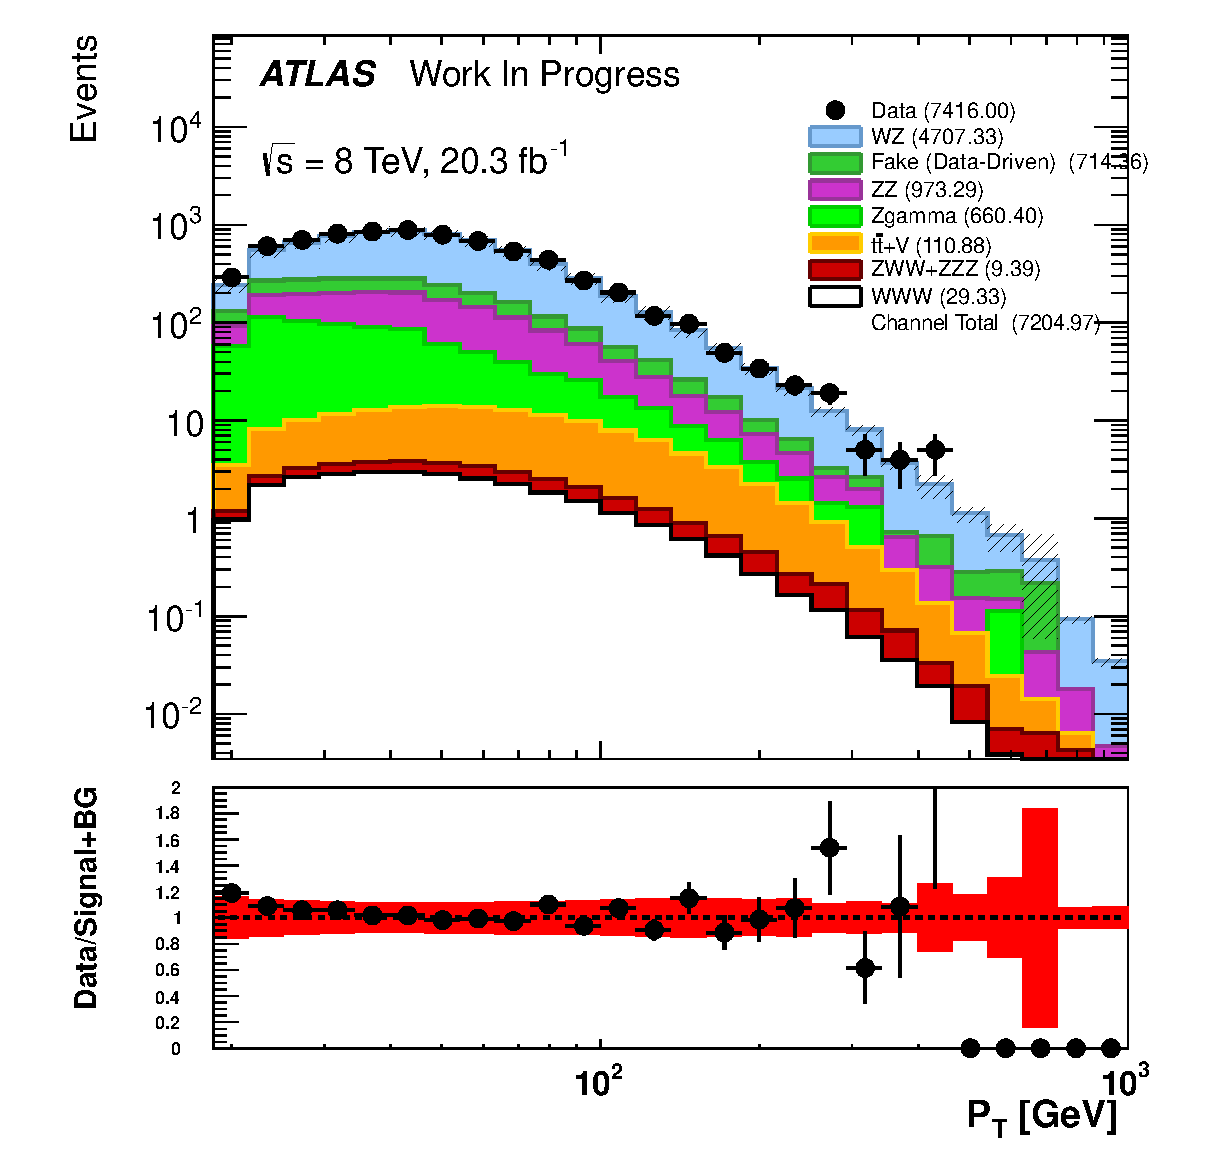
\includegraphics[width=0.3\columnwidth]{figures/appendix_signal_selection/Nov24Update_FakeSys_KFacSys_LogY_NoRebin/output/jobs/MxM/DataFull_Rates_May13_FakeRatesExactly2Loose_MuonMxMBJetGt0_ElBJetGt0SubtractPC_MxM/PreselectionNov23_15_physics/weight_all/eps/AllLeptonPt_histratio.eps}
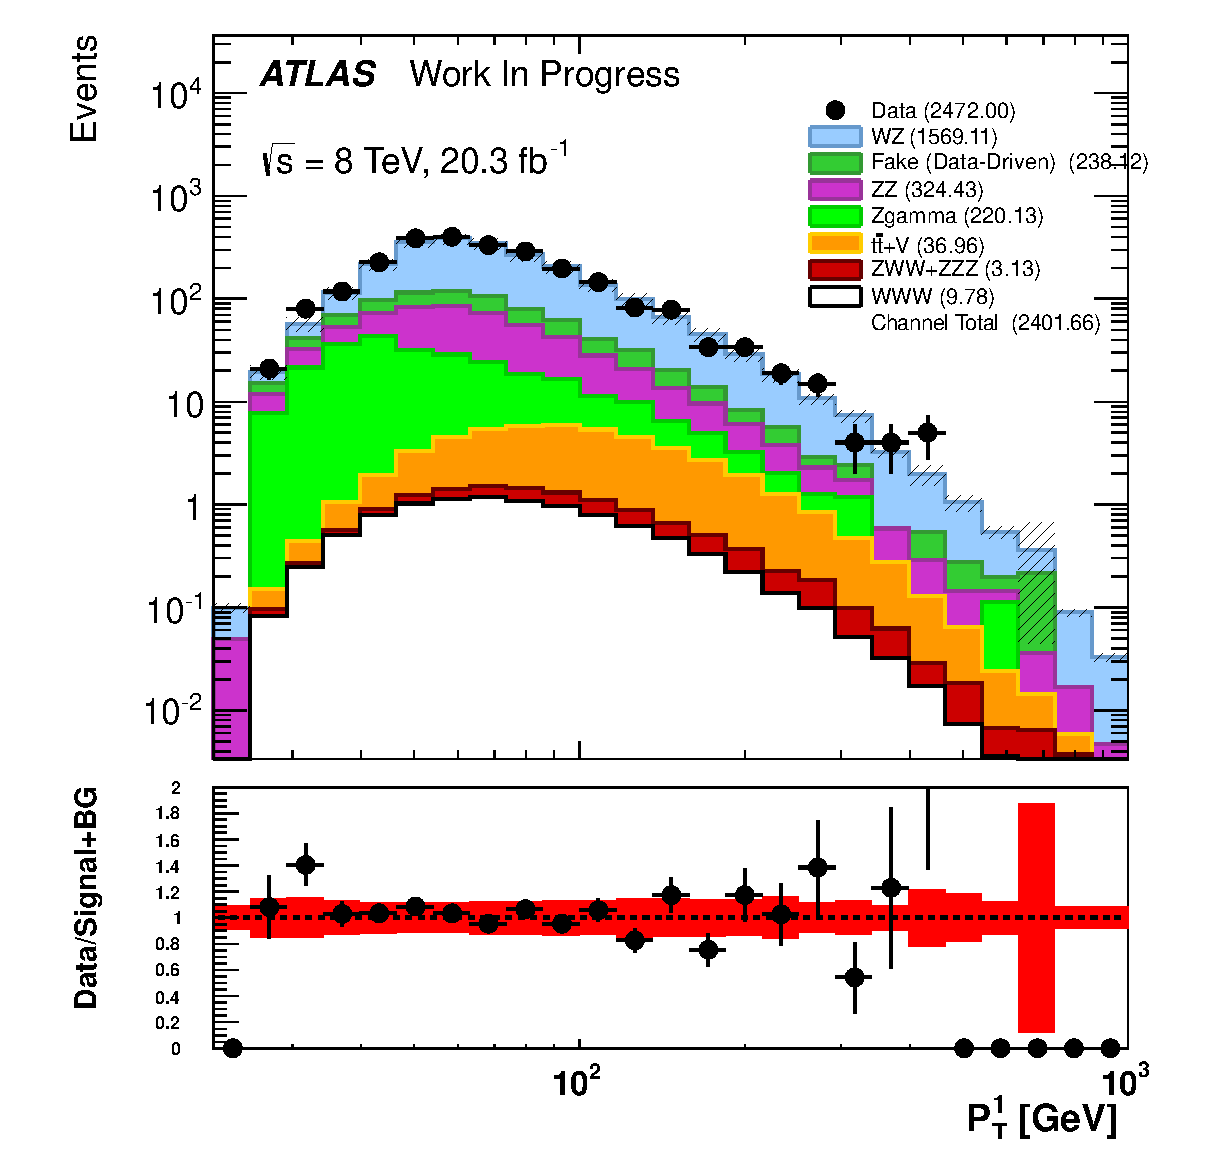
\includegraphics[width=0.3\columnwidth]{figures/appendix_signal_selection/Nov24Update_FakeSys_KFacSys_LogY_NoRebin/output/jobs/MxM/DataFull_Rates_May13_FakeRatesExactly2Loose_MuonMxMBJetGt0_ElBJetGt0SubtractPC_MxM/PreselectionNov23_15_physics/weight_all/eps/LeadingLeptonPt_histratio.eps}
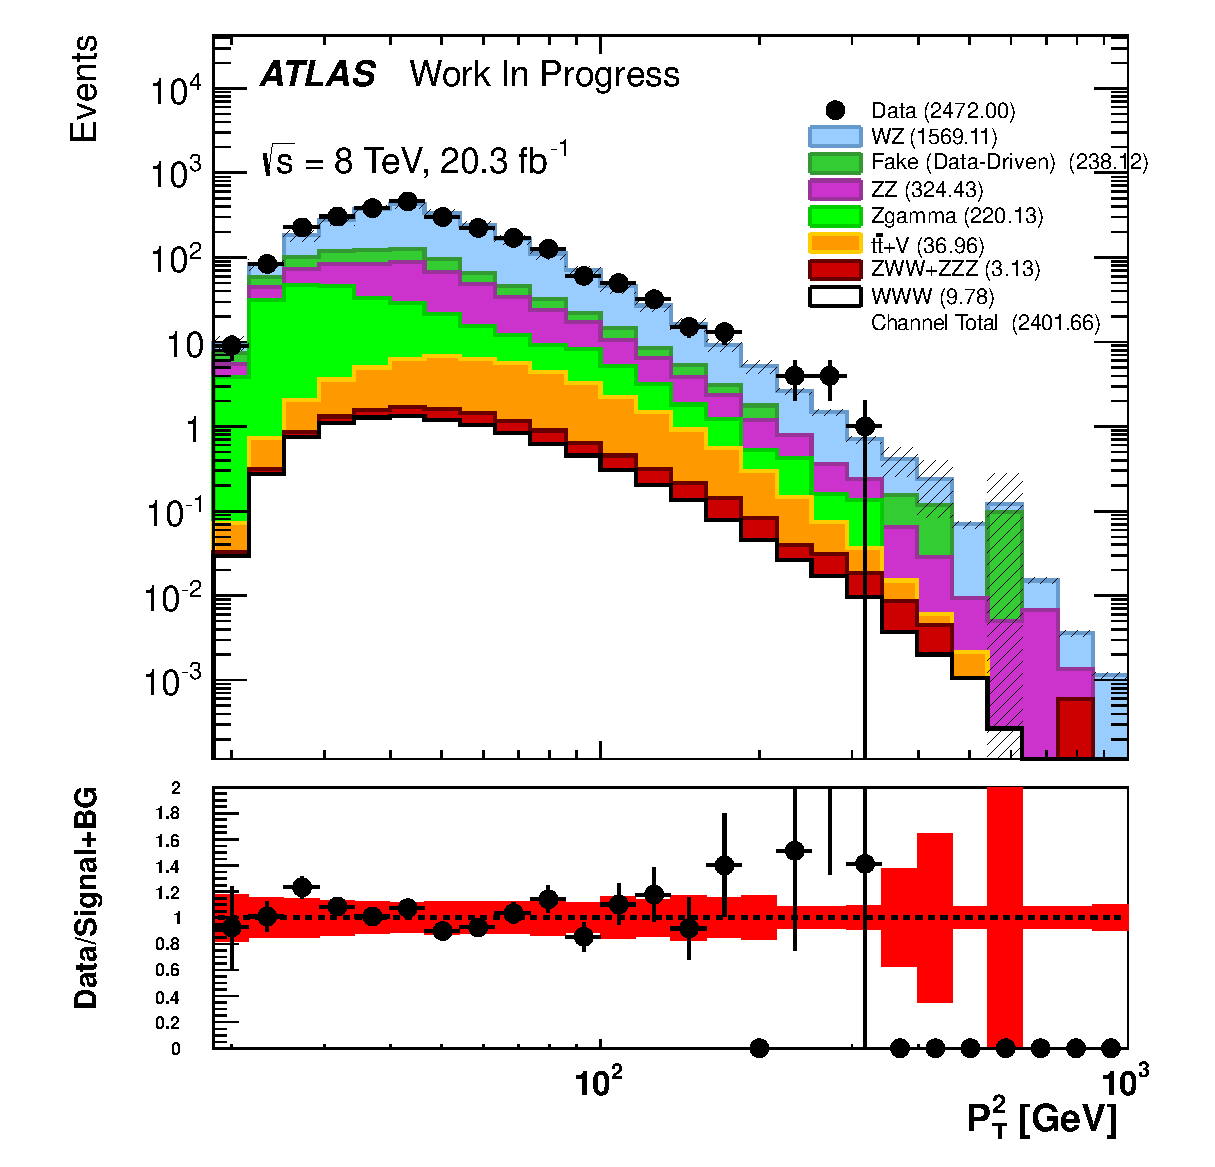
\includegraphics[width=0.3\columnwidth]{figures/appendix_signal_selection/Nov24Update_FakeSys_KFacSys_LogY_NoRebin/output/jobs/MxM/DataFull_Rates_May13_FakeRatesExactly2Loose_MuonMxMBJetGt0_ElBJetGt0SubtractPC_MxM/PreselectionNov23_15_physics/weight_all/eps/SubleadingLeptonPt_histratio.eps}
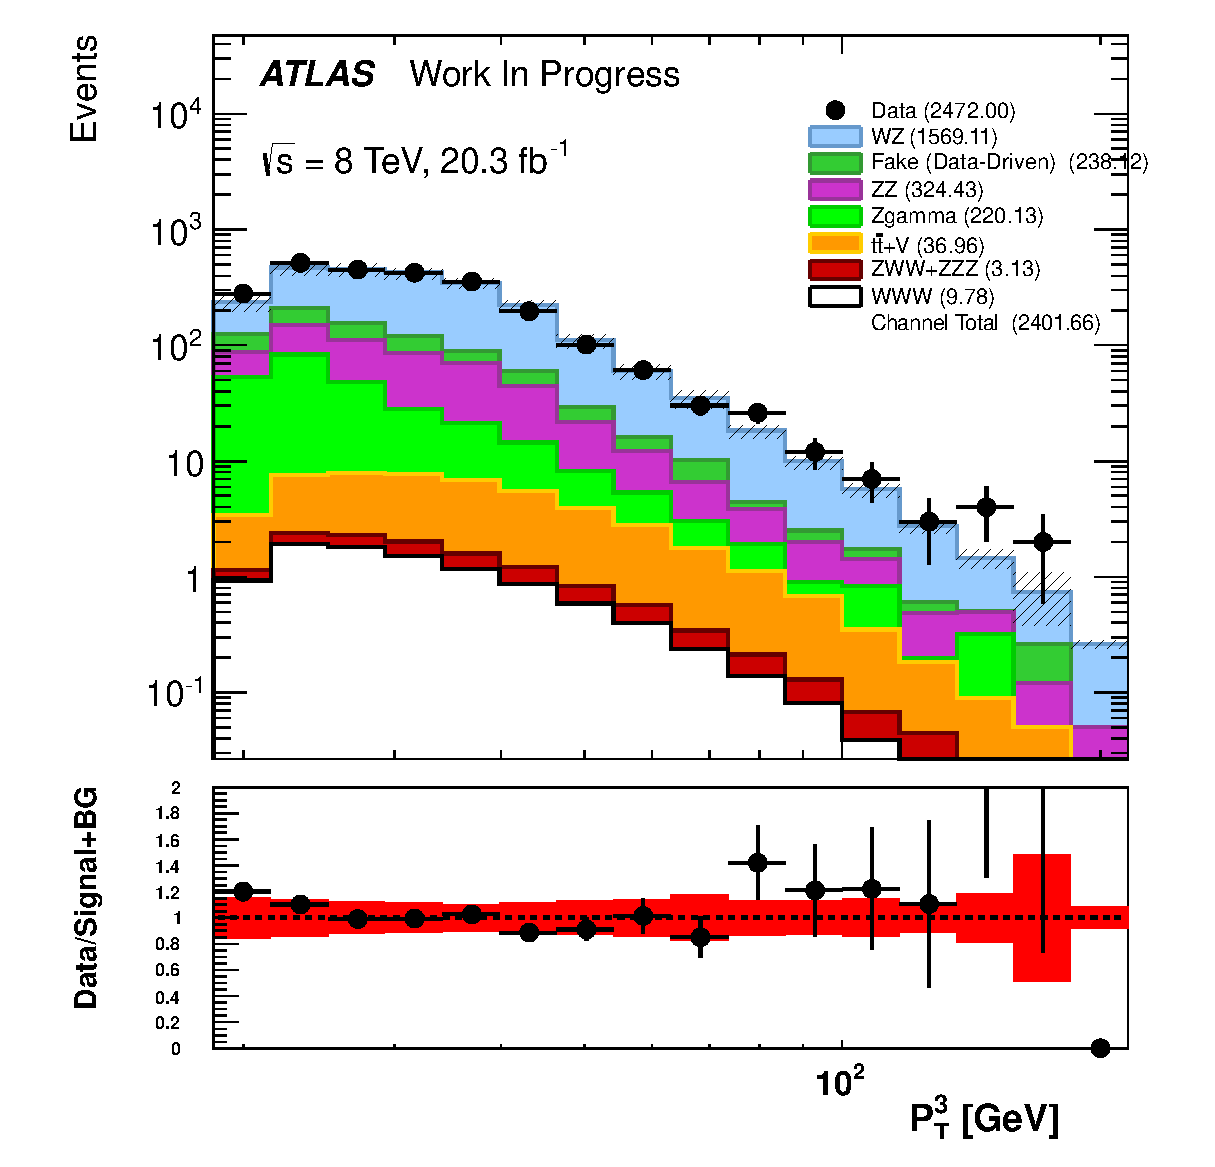
\includegraphics[width=0.3\columnwidth]{figures/appendix_signal_selection/Nov24Update_FakeSys_KFacSys_LogY_NoRebin/output/jobs/MxM/DataFull_Rates_May13_FakeRatesExactly2Loose_MuonMxMBJetGt0_ElBJetGt0SubtractPC_MxM/PreselectionNov23_15_physics/weight_all/eps/MinimumLeptonPt_histratio.eps}
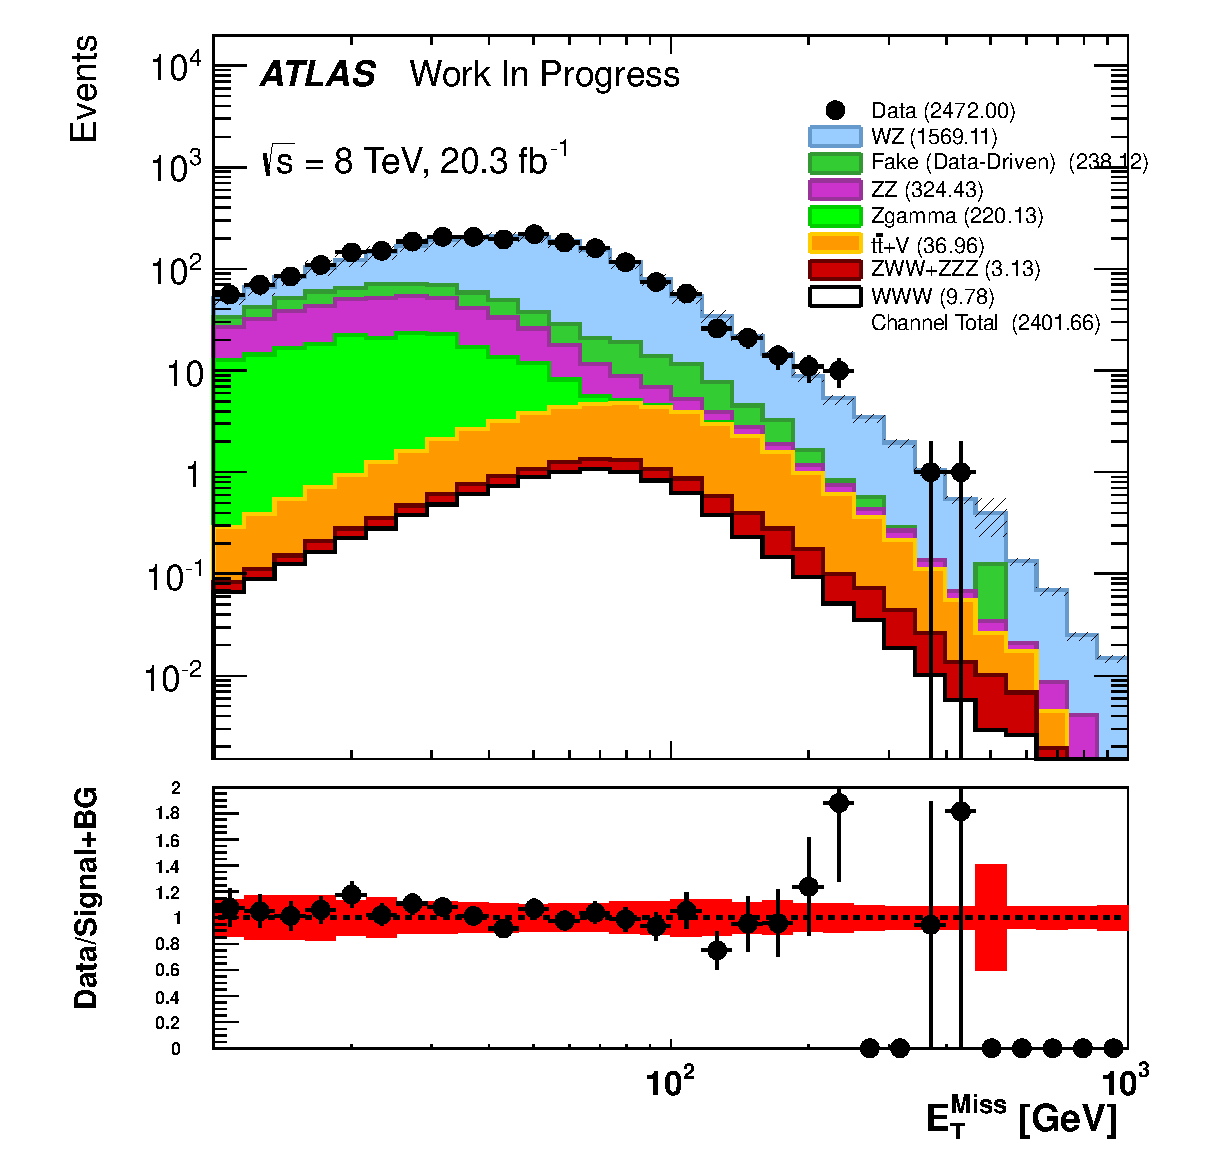
\includegraphics[width=0.3\columnwidth]{figures/appendix_signal_selection/Nov24Update_FakeSys_KFacSys_LogY_NoRebin/output/jobs/MxM/DataFull_Rates_May13_FakeRatesExactly2Loose_MuonMxMBJetGt0_ElBJetGt0SubtractPC_MxM/PreselectionNov23_15_physics/weight_all/eps/MET_Et_histratio.eps}
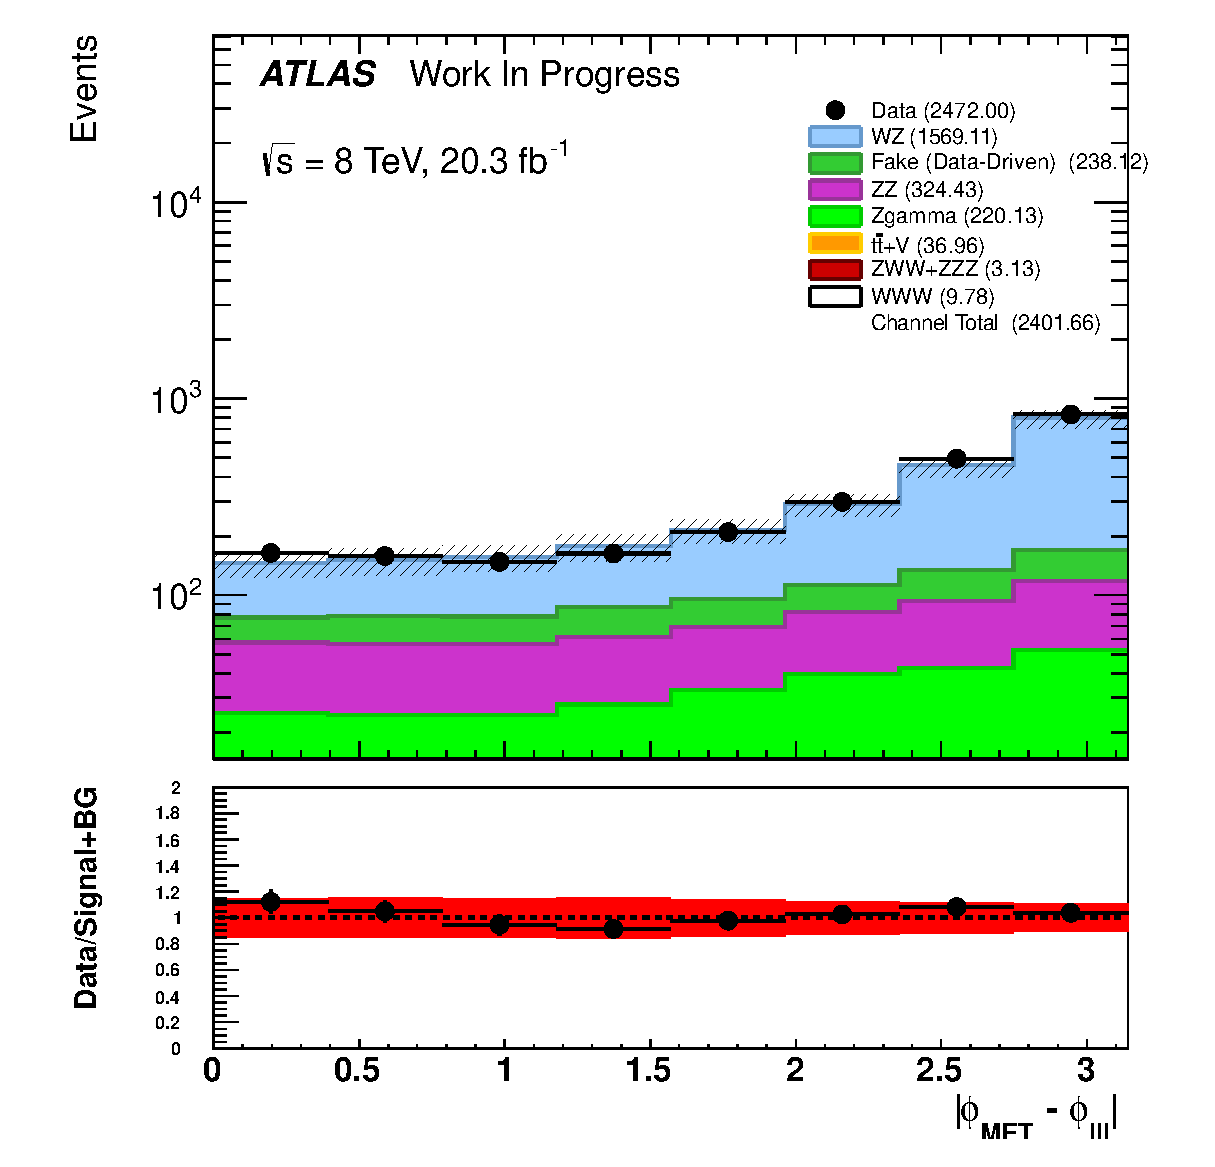
\includegraphics[width=0.3\columnwidth]{figures/appendix_signal_selection/Nov24Update_FakeSys_KFacSys_LogY_NoRebin/output/jobs/MxM/DataFull_Rates_May13_FakeRatesExactly2Loose_MuonMxMBJetGt0_ElBJetGt0SubtractPC_MxM/PreselectionNov23_15_physics/weight_all/eps/DeltaPhiMET123_Abs_histratio.eps}
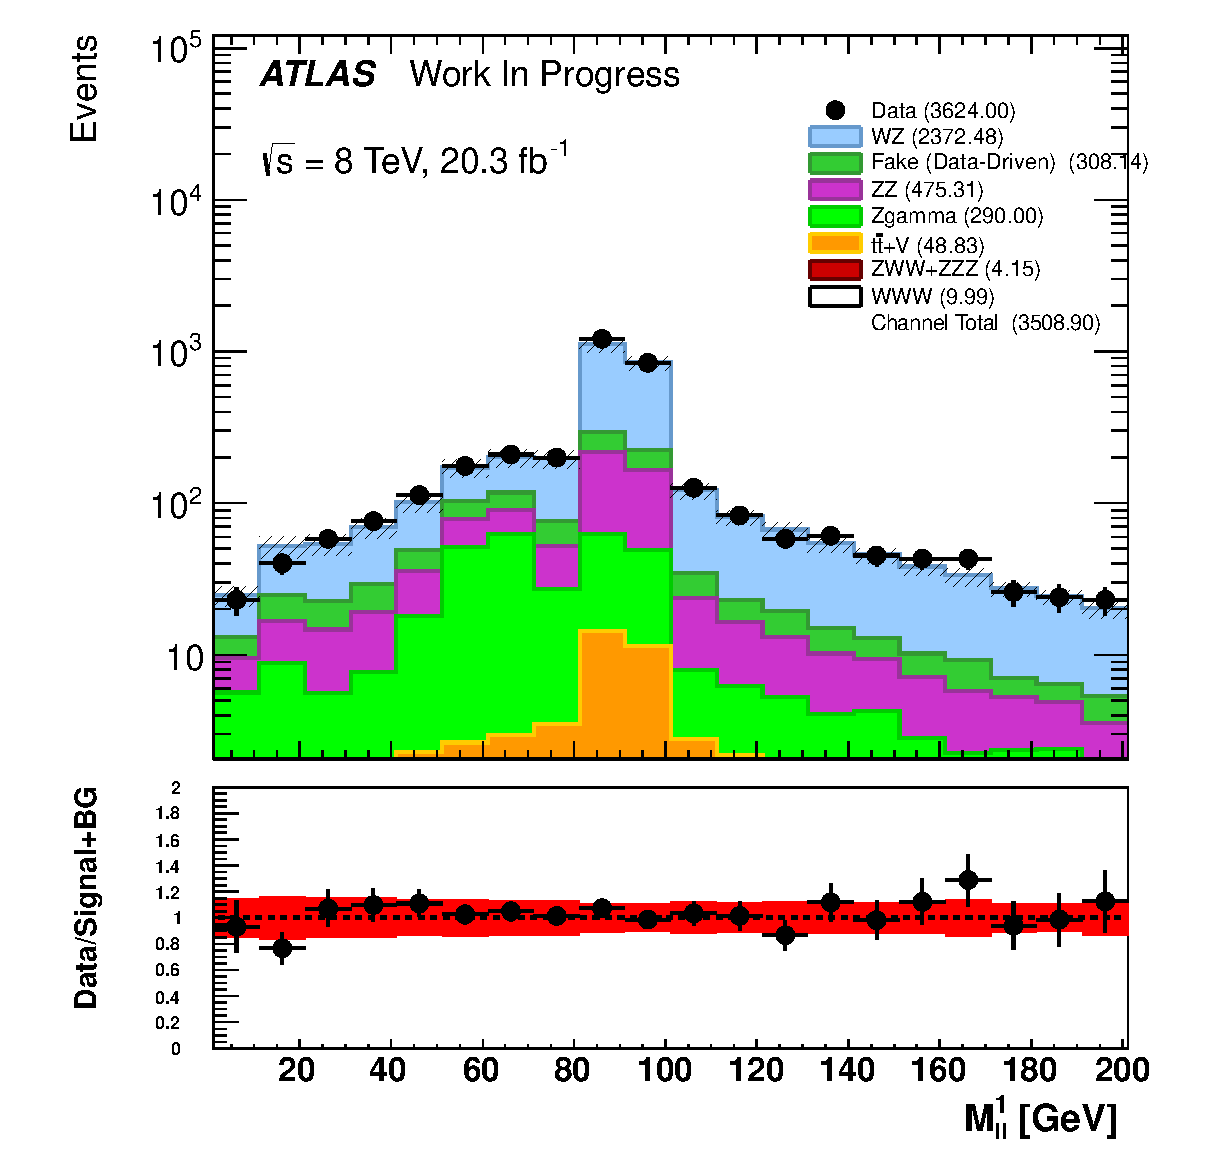
\includegraphics[width=0.3\columnwidth]{figures/appendix_signal_selection/Nov24Update_FakeSys_KFacSys_LogY_NoRebin/output/jobs/MxM/DataFull_Rates_May13_FakeRatesExactly2Loose_MuonMxMBJetGt0_ElBJetGt0SubtractPC_MxM/PreselectionNov23_15_physics/weight_all/eps/InvariantMassSFOS_histratio.eps}
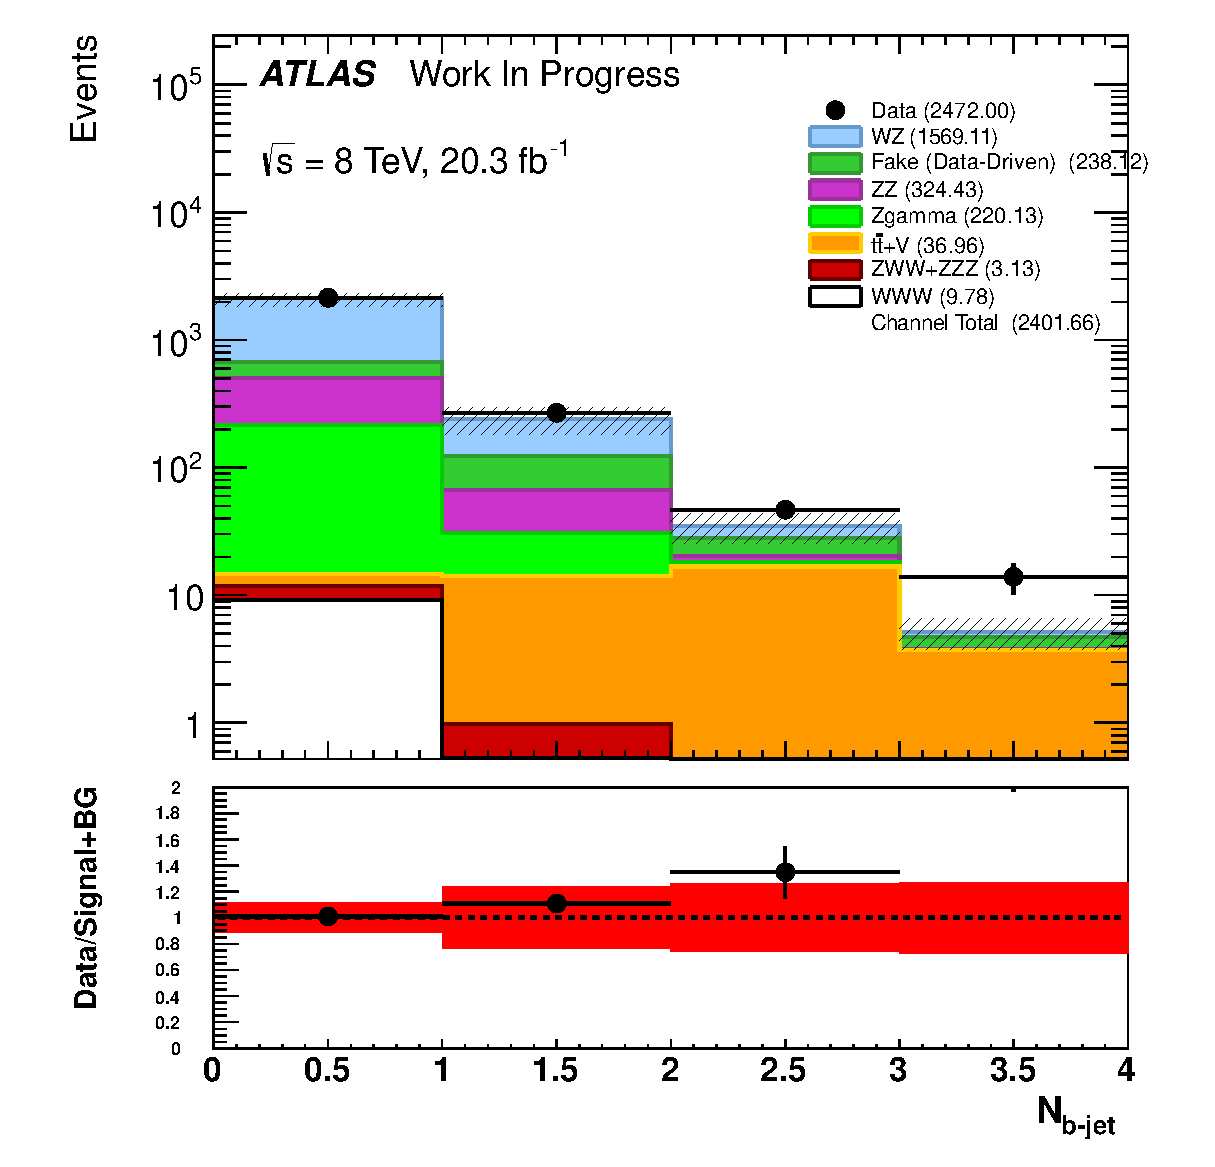
\includegraphics[width=0.3\columnwidth]{figures/appendix_signal_selection/Nov24Update_FakeSys_KFacSys_LogY_NoRebin/output/jobs/MxM/DataFull_Rates_May13_FakeRatesExactly2Loose_MuonMxMBJetGt0_ElBJetGt0SubtractPC_MxM/PreselectionNov23_15_physics/weight_all/eps/NBTaggedJets_histratio.eps}
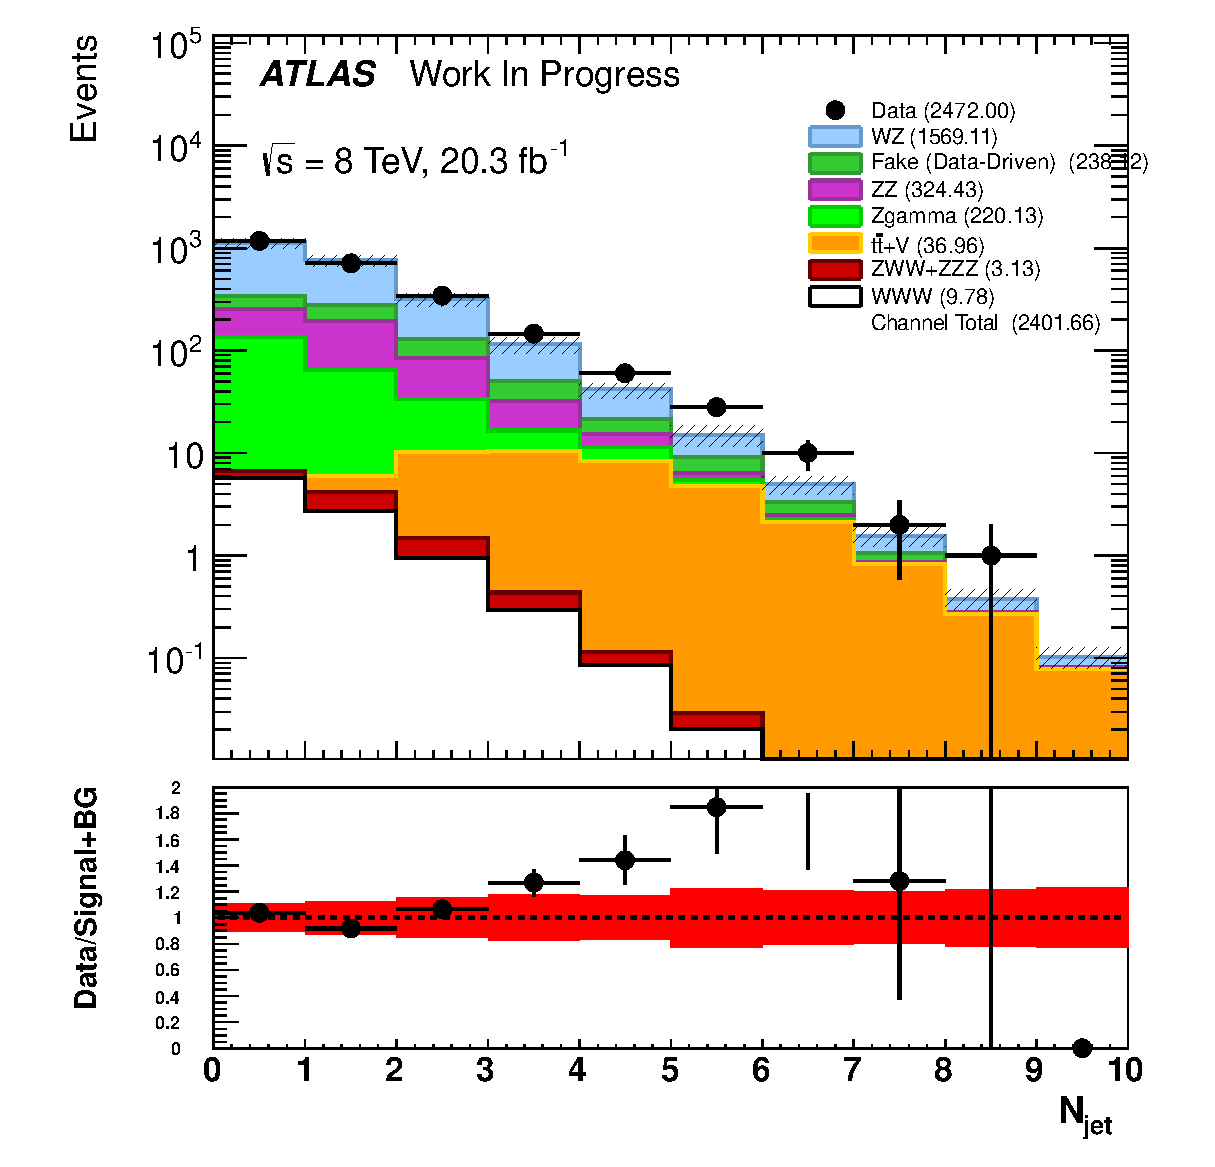
\includegraphics[width=0.3\columnwidth]{figures/appendix_signal_selection/Nov24Update_FakeSys_KFacSys_LogY_NoRebin/output/jobs/MxM/DataFull_Rates_May13_FakeRatesExactly2Loose_MuonMxMBJetGt0_ElBJetGt0SubtractPC_MxM/PreselectionNov23_15_physics/weight_all/eps/NJets_histratio.eps}
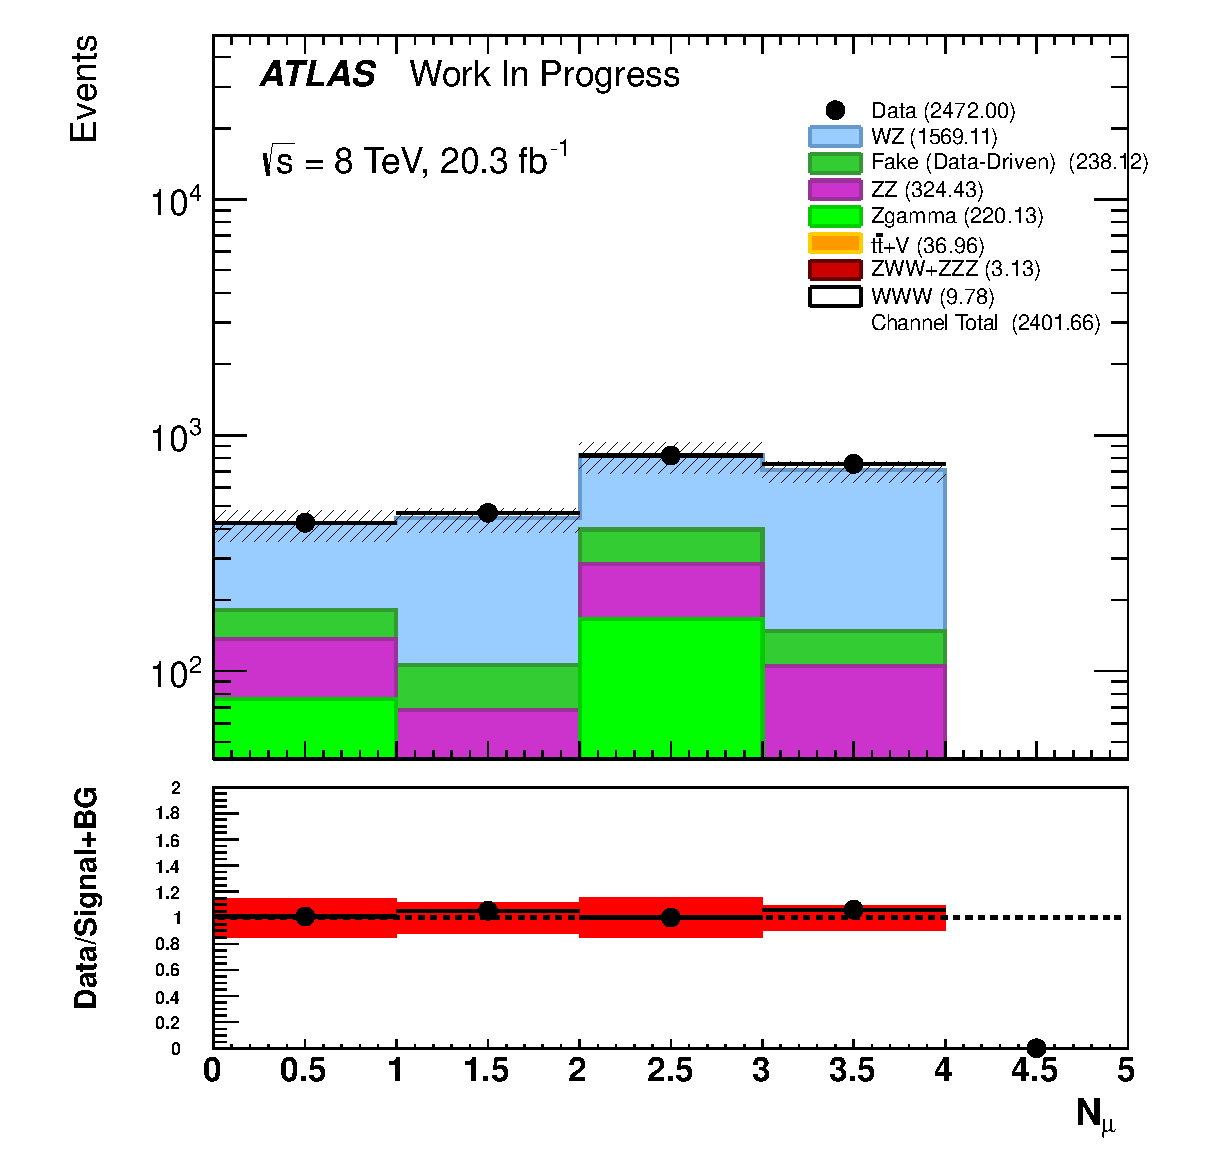
\includegraphics[width=0.3\columnwidth]{figures/appendix_signal_selection/Nov24Update_FakeSys_KFacSys_LogY_NoRebin/output/jobs/MxM/DataFull_Rates_May13_FakeRatesExactly2Loose_MuonMxMBJetGt0_ElBJetGt0SubtractPC_MxM/PreselectionNov23_15_physics/weight_all/eps/NMuons_histratio.eps}
%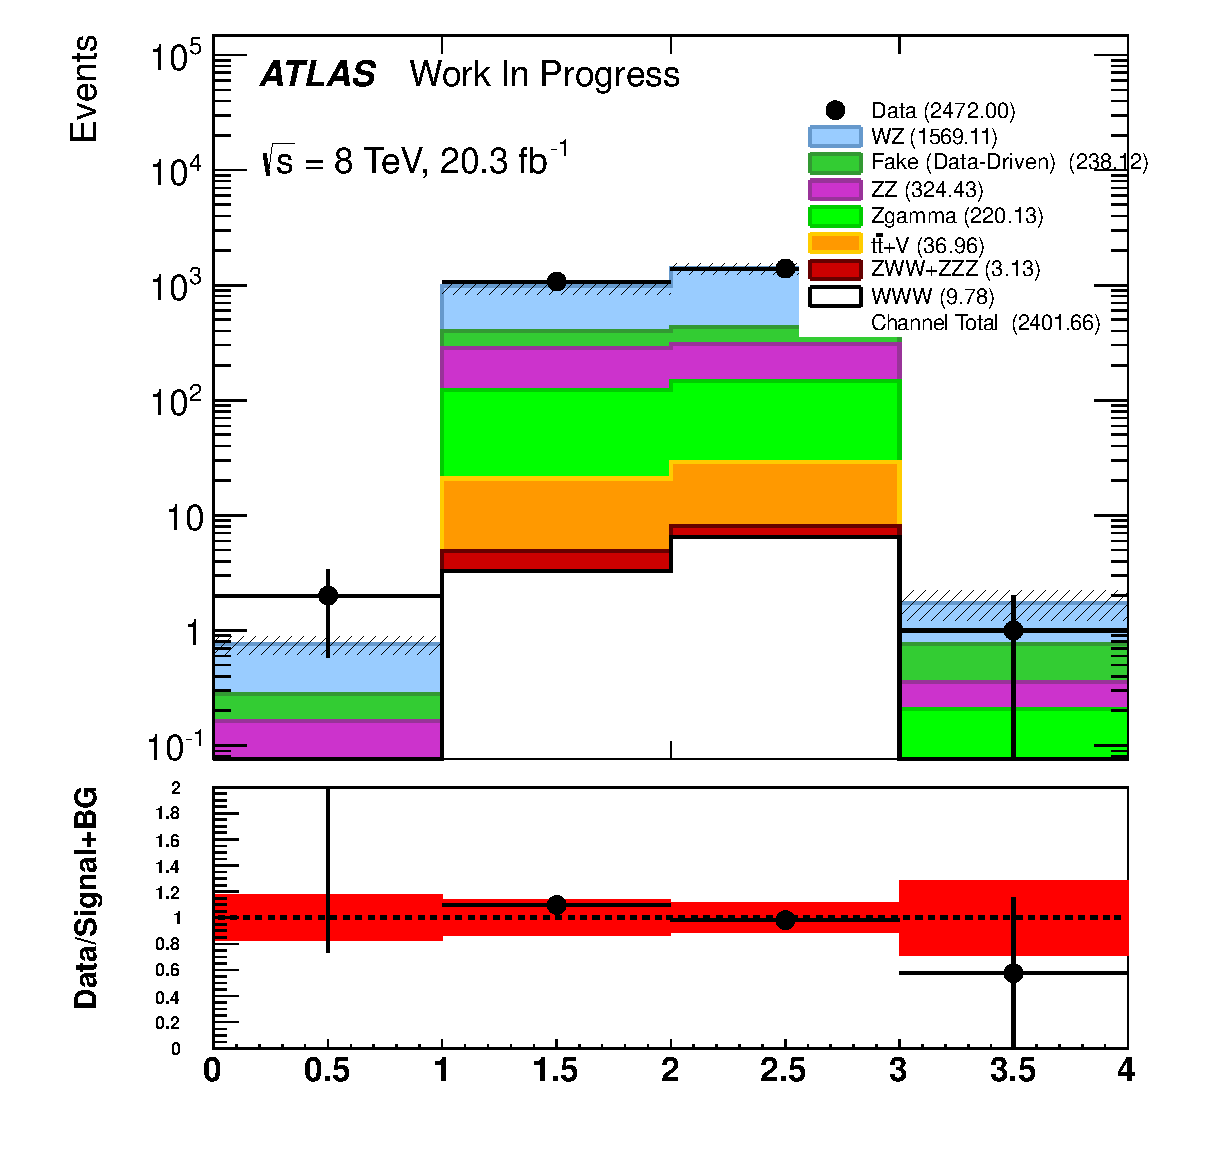
\includegraphics[width=0.3\columnwidth]{figures/appendix_signal_selection/Nov24Update_FakeSys_KFacSys_LogY_NoRebin/output/jobs/MxM/DataFull_Rates_May13_FakeRatesExactly2Loose_MuonMxMBJetGt0_ElBJetGt0SubtractPC_MxM/PreselectionNov23_15_physics/weight_all/eps/TotalCharge_histratio.eps}
\caption{Distributions showing the observed data compared to the background estimate at event pre-selection.
From top to bottom and left to right, these distributions are: the leading, 
sub-leading, and minimum lepton \pt~(ordered by their \pt), 
\MET, \deltaphi, $m_{\textrm{SFOS}}$, \njet, \nbjet, and $N_{\mu}$.
}
\label{fig:preselection}
\end{figure}
The signal plus background model 
(described in detail in \sec\ref{sec:bg_estimates})
is compared to data at pre-selection, defined in \sec\ref{sec:preselection},
for a few different kinematic distributions 
in \fig\ref{fig:preselection}. In the upper plot of each distribution,
the colored histograms 
represent the different categories contributing to the signal 
plus background model and 
are split by color based on the category. 
%The colors are...
Hashed bands are shown on the stacked
histograms representing the size of the systematic uncertainties 
on the model, described in \sec\ref{sec:systematics}.
The data is shown in the black points where the 
bars on the points represent the statistical uncertainty on the data.
The lower plot shows the ratio of the data over the model.
In this case, the error bars correspond to the statistical uncertainty
on the ratio due to both the data and the model. The red band
shows the size of the systematic uncertainties with respect to the model.
The model is said to be consistent with the data
if the ratio is compatible with unity after considering statistical
and systematic uncertainties.
The different distributions are chosen primarily because 
of their potential to discriminate between signal and background. 
The signal plus background model is observed to be consistent
with the data at pre-selection. 




%\begin{table}[ht!]
%\centering
%\begin{tabular}{|c||c|c|c|c|}
\hline
 & $eee$ & $ee\mu$ & $e\mu\mu$ & $\mu\mu\mu$\\ 
\hline\hline
$WZ$ &  $240.85 \pm 0.67$ &  $339.17 \pm 0.82$ &  $422.07 \pm 0.87$ &  $567.0 \pm 1$\\ 
$ZZ$ &  $60.21 \pm 0.13$ &  $54.1 \pm 0.2$ &  $118.60 \pm 0.31$ &  $91.48 \pm 0.17$\\ 
$Z\gamma$ &  $70.1 \pm 2.7$ &  $0.47 \pm 0.22$ &  $149.4 \pm 3.9$ &  $0.17 \pm 0.12$\\ 
$ZWW+ZZZ$ &  $0.436 \pm 0.019$ &  $0.834 \pm 0.027$ &  $1.00 \pm 0.03$ &  $0.864 \pm 0.028$\\ 
$t\bar{t}+V$ &  $4.854 \pm 0.044$ &  $9.549 \pm 0.064$ &  $12.047 \pm 0.072$ &  $10.510 \pm 0.066$\\ 
Fake (data-driven) &  $45.1 \pm 2.2$ &  $37.8 \pm 1.6$ &  $112.7 \pm 2.8$ &  $42.5 \pm 1.2$\\ 
$WWW$ &  $0.770 \pm 0.011$ &  $3.023 \pm 0.023$ &  $3.970 \pm 0.026$ &  $1.843 \pm 0.018$\\ 
\hline
Expected Background &  $421.6 \pm 3.5$ &  $441.9 \pm 1.8$ &  $815.8 \pm 4.9$ &  $712.5 \pm 1.6$\\ 
Expected Signal + Background &  $422.4 \pm 3.5$ &  $444.9 \pm 1.8$ &  $819.8 \pm 4.9$ &  $714.4 \pm 1.6$\\ 
\hline
Observed Data &  $426 \pm 21$ &  $468 \pm 22$ &  $821 \pm 29$ &  $757 \pm 28$\\ 
\hline
\end{tabular}

%\caption{Expected and observed event yields binned by lepton flavor combination at event pre-selection.
%Only statistical uncertainties are shown.
%}
%\label{tab:preselection}
%\end{table}



\begin{figure}[ht!]
\centering
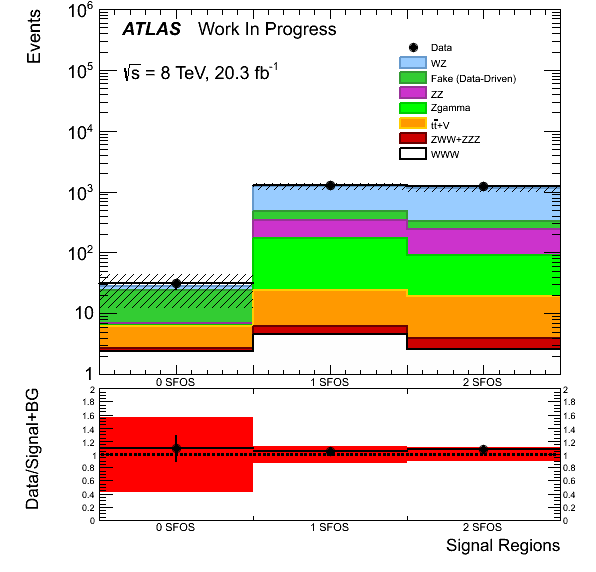
\includegraphics[width=0.5\columnwidth]{figures/SFOSPreselection.png}
\caption{Yields at event pre-selection in the 0, 1 and 2 SFOS regions.  
The most important systematic uncertainties 
(discussed in section~\ref{sec:systematics}) are shown, 
namely from the fake estimates and the uncertainties on the WZ and ZZ k-factors.}
\label{fig:preselection_nsfos}
\end{figure}

Upon splitting the pre-selection region based on the number of SFOS
pairs, we end up with the signal and background predictions in
\fig\ref{fig:preselection_nsfos}, where we can see differences
in the branching fraction for the signal to fall into
each of the three signal regions.
In the 0 and 2 SFOS regions, roughly 2.5 signal events are predicted
whereas closer to 5 signal events are predicted in the 1 SFOS region,
totaling about 10 signal events predicted at the pre-selection stage.
Shifting to looking at the background, perhaps the most striking 
feature of this plot is the 
clear difference in background yield and background composition
between the 0 SFOS region and the 1 and 2 SFOS regions.
More than 1000 background events are predicted in both the 1 and
the 2 SFOS regions, but only about 30 background events are
predicted in the 0 SFOS region.
Clearly then, the advantage of splitting the signal region based on this
classification comes when looking at the background, specifically the
electroweak $WZ$ and $ZZ$ backgrounds where SFOS lepton pairs may be
produced from the decay of the $Z$ boson(s). Consider only the case
where the $WZ$ and $ZZ$ decay to either $e$ or $\mu$.  The $WZ$ production
process is thus characterized by 3 leptons with at least 1 SFOS lepton pair
which comes from the $Z$. If all three leptons from the $WZ$ decay have been
reconstructed, then there is a 50~\% chance the third lepton 
will also be able to form a SFOS pair with one of the leptons from the $Z$ decay.
Thus, the WZ background will split evenly between the 1 and 2 SFOS classification.
Something similar occurs for the ZZ background except that the fourth lepton 
in the decay must be lost (usually due to possessing a low $\pt$).
The large cross-section for these processes means that
they become the dominant backgrounds in the 1 and 2 SFOS regions.  
The 0 SFOS signal region is mostly spared from contamination  by 
these large processes but still
includes both the $WZ$ and $ZZ$ processes as background due to the
non-negligible (albeit small) effect of mis-measurement of the electron
charge described in \sec\ref{sec:charge_misid}.  The 0 SFOS signal region
is thus unique in having a small background which is almost entirely
reducible and dominated instead by the fake background,
described in \sec\ref{sec:bg_fake},
along with the aforementioned sub-dominant effect of electron charge 
mis-identification.

\subsection{Optimization}
\label{sec:optimization}

A more stringent selection must be applied on top of the pre-selection
in \sec\ref{sec:preselection_yield} in order to obtain any
sensitivity to the signal.  The best selection, however, is
not known \emph{a priori}. We try to find the best possible selection
by starting from a list of kinematic quantities, chosen based on heuristic
arguments. These kinematic quantities, along with the signal
plus background model, are passed into an optimization 
framework that systematically seeks to simultaneously 
maximize the predicted signal and the precision on the final measurement.

The optimization framework considers independent permutations of the different
kinematic quantities, along with variations of the selection thresholds
on these cuts, to form combinations of selection cuts which could become a final
selection. For each combination, or operating point,
that is considered, the signal plus background
model is evaluated to determine the expected yields and systematic
uncertainties given that selection.  The LHC data is not used in the optimization.  
The prediction is then plugged into the statistical framework described in
\sec\ref{sec:measurement} to extract a value on the expected precision
of the measurement. For each operating point,
the value on the precision is plotted against the expected signal yield.
With some discretion, we then choose the operating point 
that maximized the signal yield and gives the smallest absolute 
precision on the measurement. 


The selection thresholds considered are...

We split by signal region...

The different operating points look like...


Some of the intuition for this can be understood by looking at individual
distributions...

this results in the selection of table blah...

\subsection{Signal Region Yields}
\label{sec:signal_yield}
\begin{figure}[ht!]
\centering
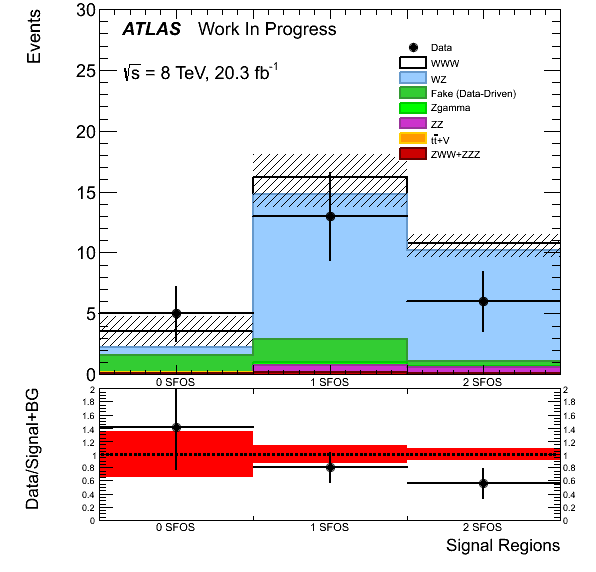
\includegraphics[width=0.5\columnwidth]{figures/SFOSSignalRegions.png}
\caption{Yields after full selection in the 0, 1 and 2 SFOS regions.  
The most important systematic uncertainties are shown, namely from the 
fake estimates and the uncertainties on the WZ and ZZ k-factors.}
\label{fig:sig_yields_nsfos}
\end{figure}

The optmized signal region selection
described in \sec\ref{sec:optimization} and \sec\ref{sec:signal_regions}
and listed in \tab\ref{tab:signal_selection} is applied 
to the data as well as the signal plus background model.
A plot of the predicted yields for the 
signal plus background, along with systematic uncertainties,
is compared to the data for each signal region
in \fig\ref{fig:sig_yields_nsfos}. A detailed 
breakdown of the predicted yields and overall uncertainties
on each background as well as the signal prediction and observed
data
are presented in \tab\ref{tab:sys_summary}.
A breakdown of the systematic uncertainty contributions
to the signal and the backgrounds in each signal region
are summarized in \tab\ref{tab:sys_breakdown}.
More details are presented about each signal region below.



\begin{table}[ht!]
\centering
\renewcommand{\tabcolsep}{2pt}
\small\begin{tabular}{c|rclrclrcl}
\hline
\hline
 & \multicolumn{3}{c}{0 SFOS} & \multicolumn{3}{c}{1 SFOS} & \multicolumn{3}{c}{2 SFOS}\\ 
\hline
$WZ$ &  $0.6176 $&$\pm$&$ 0.0043~^{+0.0699}_{-0.0701}$ &  $11.89 $&$\pm$&$ 0.14~^{+1.32}_{-1.29}$ &  $9.05 $&$\pm$&$ 0.13~^{+0.99}_{-1.00}$\\ 
ZZ &  $0.0658 $&$\pm$&$ 0.0039~^{+0.0112}_{-0.0112}$ &  $0.581 $&$\pm$&$ 0.016~^{+0.106}_{-0.105}$ &  $0.477 $&$\pm$&$ 0.011~^{+0.095}_{-0.086}$\\ 
$WWZ+WZZ$ &  $0.1126 $&$\pm$&$ 0.0099~^{+0.0146}_{-0.0117}$ &  $0.140 $&$\pm$&$ 0.011~^{+0.015}_{-0.013}$ &  $0.0785 $&$\pm$&$ 0.0080~^{+0.0097}_{-0.0106}$\\ 
$t\overline{t}+$V &  $0.0388 $&$\pm$&$ 0.0043~^{+0.0061}_{-0.0077}$ &  $0.0503 $&$\pm$&$ 0.0048~^{+0.0074}_{-0.0089}$ &  $0.0239 $&$\pm$&$ 0.0033~^{+0.0074}_{-0.0058}$\\ 
DPS &  $0.0 $&$\pm$&$ 0.0~^{+0.0}_{-0.0}$ &  $0.0088 $&$\pm$&$ 0.0080~^{+0.0080}_{-0.0084}$ &  $0.023 $&$\pm$&$ 0.016~^{+0.019}_{-0.029}$\\ 
$Z\gamma$ &  $0.0 $&$\pm$&$ 0.0~^{+0.0}_{-0.0}$ &  $0.20 $&$\pm$&$ 0.13~^{+0.29}_{-0.13}$ &  $0.110 $&$\pm$&$ 0.096~^{+0.163}_{-0.288}$\\ 
Fake &  $1.51 $&$\pm$&$ 0.26~^{+1.40}_{-1.29}$ &  $1.90 $&$\pm$&$ 0.34~^{+1.90}_{-1.77}$ &  $0.49 $&$\pm$&$ 0.16~^{+0.47}_{-0.46}$\\ 
Signal &  $1.320 $&$\pm$&$ 0.015~^{+0.072}_{-0.078}$ &  $1.369 $&$\pm$&$ 0.015~^{+0.072}_{-0.080}$ &  $0.603 $&$\pm$&$ 0.010~^{+0.031}_{-0.035}$\\ 
\hline
Total Background &  $2.35 $&$\pm$&$ 0.26~^{+1.40}_{-1.30}$ &  $14.77 $&$\pm$&$ 0.39~^{+2.36}_{-2.22}$ &  $10.25 $&$\pm$&$ 0.23~^{+1.15}_{-1.22}$\\ 
Total Predicted &  $3.67 $&$\pm$&$ 0.26~^{+1.41}_{-1.30}$ &  $16.14 $&$\pm$&$ 0.39~^{+2.33}_{-2.18}$ &  $10.86 $&$\pm$&$ 0.23~^{+1.12}_{-1.19}$\\ 
\hline
Data &  \multicolumn{3}{c}{$5$} &  \multicolumn{3}{c}{$13$} &  \multicolumn{3}{c}{$6$}\\ 
\hline
\end{tabular}

\caption{A summary of the expected yields compared to data for all 
three signal regions.  Statistical uncertainties are shown 
as a symmetric uncertainty on the central value. Systematic uncertainties 
are shown as an asymmetric uncertainty and are shown
after taking the quadrature sum of all individual uncertainties. 
In the actual analysis, each systematic uncertainty is
treated as an individual nuisance paramter and are NOT added in quadrature.  
The presentation here serves only as a demonstration
of the overall size of the systematic uncertainties for each source in the 
individual signal regions.}
\label{tab:sys_summary}
\end{table}

\begin{table}[ht!]
\centering
\small
\renewcommand{\arraystretch}{1.5}
\begin{tabular}{c||ccc|ccc}
\hline

\multirow{2}{*}{Source of Uncertainty} & \multicolumn{3}{|c|}{Signal} & \multicolumn{3}{c}{Backgound} \\
 & 0 SFOS& 1 SFOS & 2 SFOS & 0 SFOS & 1 SFOS & 2 SFOS\\ 
\hline\hline
Electron &  $^{+1.56}_{-1.47}$  &  $^{+1.66}_{-1.61}$  &  $^{+1.02}_{-1.06}$  &  $^{+0.68}_{-0.69}$  &  $^{+2.34}_{-1.49}$  &  $^{+1.05}_{-1.54}$ \\ 
Muon &  $^{+0.56}_{-0.54}$  &  $^{+0.54}_{-0.54}$  &  $^{+0.74}_{-0.83}$  &  $^{+0.19}_{-0.19}$  &  $^{+1.09}_{-0.48}$  &  $^{+0.81}_{-0.80}$ \\ 
MET &  $^{+1.38}_{-1.75}$  &  $^{+0.71}_{-0.89}$  &  $^{+0.23}_{-0.35}$  &  $^{+0.79}_{-0.73}$  &  $^{+1.38}_{-0.11}$  &  $^{+2.12}_{-2.66}$ \\ 
Jet &  $^{+2.36}_{-2.26}$  &  $^{+2.06}_{-2.34}$  &  $^{+1.56}_{-2.22}$  &  $^{+1.10}_{-1.06}$  &  $^{+2.74}_{-2.03}$  &  $^{+2.94}_{-4.41}$ \\ 
Trigger &  $^{+0.09}_{-0.09}$  &  $^{+0.09}_{-0.09}$  &  $^{+0.20}_{-0.20}$  &  $^{+0.06}_{-0.06}$  &  $^{+0.09}_{-0.09}$  &  $^{+0.21}_{-0.21}$ \\ 
Matrix Method & --- & --- & --- &  $^{+58.56}_{-53.98}$  &  $^{+12.64}_{-11.78}$  &  $^{+4.34}_{-4.23}$ \\ 
Charge Mis-ID & --- & --- & --- &  $^{+0.45}_{-0.44}$  & --- & ---\\ 
Pileup &  $^{+0.92}_{-0.77}$  &  $^{+1.10}_{-1.30}$  &  $^{+1.50}_{-1.24}$  &  $^{+0.52}_{-0.42}$  &  $^{+0.22}_{+0.00}$  &  $^{+1.39}_{-1.40}$ \\ 
Luminosity &  $^{+2.80}_{-2.80}$  &  $^{+2.80}_{-2.80}$  &  $^{+2.80}_{-2.80}$  &  $^{+2.80}_{-2.80}$  &  $^{+2.80}_{-2.80}$  &  $^{+2.80}_{-2.80}$ \\ 
Theory &  $^{+5.55}_{-3.75}$  &  $^{+5.55}_{-3.75}$  &  $^{+5.55}_{-3.75}$  &  $^{+2.66}_{-2.66}$  &  $^{+8.07}_{-8.07}$  &  $^{+8.85}_{-8.85}$ \\ 
Statistical &  $^{+1.14}_{-1.14}$  &  $^{+1.12}_{-1.12}$  &  $^{+1.70}_{-1.70}$  &  $^{+10.99}_{-10.99}$  &  $^{+2.67}_{-2.67}$  &  $^{+2.20}_{-2.20}$ \\ 
\hline
\end{tabular}

\caption{Categorized systematic uncertainties 
for signal and background predictions in all three signal regions.
All uncertainties are shown as a percentage of the nominal
prediction.  }
\label{tab:sys_breakdown}
\end{table}


\clearpage
\subsubsection{0 SFOS Signal Region}



\begin{table}[ht!]
\centering
\small
\begin{tabular}{l||c|c||c|c||c|c}
\hline
 &                 \multicolumn{2}{c||}{Signal}            &  \multicolumn{2}{c||}{Background} &  \multicolumn{2}{c}{Data} \\
  & Yield & Eff. & Yield & Eff. & Yield & Eff.\\
  \hline\hline
  1. Pre-selection &  $9.78$ & --- &  $2388.48$ & --- & $2472$ &  --- \\ 
  \hline
  2. 0 SFOS &  $2.31$ &  $0.24$ &  $21.36$ &  $0.0089$ & $30$ &  $0.01$\\ 
  \hline
  3. Charge Sum $= \pm 1$ &  $2.30$ &  $1.00$ &  $19.55$ &  $0.92$ & $27$ &  $0.90$\\ 
  \hline
  4. $N_{\mathrm{b-jet}} = 0$ &  $2.29$ &  $0.99$ &  $8.59$ &  $0.44$ & $10$ &  $0.37$\\ 
  \hline
  5. $m_{SF} > 20$ GeV &  $2.25$ &  $0.98$ &  $8.32$ &  $0.97$ & $10$ &  $1.00$\\ 
  \hline
  6. $|m_{ee} - m_{Z}| > 15$ GeV &  $2.06$ &  $0.91$ &  $7.09$ &  $0.85$ & $9$ &  $0.90$\\ 
  \hline
  7. $|\Delta\phi(3l,E_{T}^{Miss})| > 2.5$ &  $1.41$ &  $0.69$ &  $2.51$ &  $0.35$ & $6$ &  $0.67$\\ 
  \hline
  8. $N_{\mathrm{Jet}} \leq 1$ &  $1.34$ &  $0.95$ &  $2.35$ &  $0.94$ & $5$ &  $0.83$\\ 
  \hline
  \end{tabular}


\caption{Cut-flows showing the event yields and efficiencies for each cut in the 0 SFOS signal region
starting from event pre-selection separately for the total signal and total bacgkround predictions, along with the observed data. 
Event yields for MC backgrounds and signal include all weights and are normalized to an integrated luminosity of $20.3~\mathrm{fb}^{-1}$.  
The fake lepton background only includes the matrix method weights.  The data is unweighted.
Efficiencies show the ratio of the yield with respect
to the previous cut.  The efficiency is first calculated at the first cut after event pre-selection.  }
\label{tab:cutflow_weighted_0sfos}
\end{table}

\begin{table}[ht!]
\centering
\small
\begin{tabular}{l||c|c||c|c||c|c}
\hline
 &  \multicolumn{6}{c}{Background} \\
 & \multicolumn{2}{c||}{$WZ$} & \multicolumn{2}{c||}{$ZZ$} & \multicolumn{2}{c}{$t\bar{t}+V$} \\ 
 & Yield & Eff. & Yield & Eff. & Yield & Eff. \\
\hline\hline
Pre-selection &  $1566.91$ & --- &  $323.60$ &  --- &  $36.93$ &  --- \\
\hline
0 SFOS &  $2.84$ &  $0.002$ &  $0.50$ &  $0.002$ &  $0.26$ &  $0.01$ \\
\hline
Charge Sum $= \pm 1$ &  $1.92$ &  $0.68$ &  $0.33$ &  $0.65$ &  $0.26$ &  $0.99$ \\
\hline
$N_{\mathrm{b-jet}} = 0$ &  $1.91$ &  $0.99$ &  $0.33$ &  $0.99$ &  $0.25$ &  $0.98$ \\
\hline
$m_{SF} > 20$ GeV &  $1.88$ &  $0.98$ &  $0.32$ &  $0.98$ &  $0.25$ &  $0.98$ \\
\hline
$|m_{ee} - m_{Z}| > 15$ GeV &  $1.27$ &  $0.68$ &  $0.21$ &  $0.66$ &  $0.22$ &  $0.90$ \\
\hline
$|\Delta\phi(3l,E_{T}^{Miss})| > 2.5$ &  $0.65$ &  $0.51$ &  $0.07$ &  $0.34$ &  $0.09$ &  $0.38$ \\
\hline
$N_{\mathrm{Jet}} \leq 1$ &  $0.62$ &  $0.95$ &  $0.07$ &  $0.91$ &  $0.04$ &  $0.45$ \\
\hline
\end{tabular}




\begin{tabular}{l||c|c||c|c||c|c}
\hline
 &  \multicolumn{6}{c}{Background} \\
 & \multicolumn{2}{c||}{$ZZZ+ZWW$} & \multicolumn{2}{c||}{$Z\gamma$} & \multicolumn{2}{c}{Fake}  \\ 
 & Yield & Eff. & Yield & Eff. & Yield & Eff. \\
\hline\hline
Pre-selection &  $3.12$ & --- &  $219.80$ &  --- &  $238.12$ &  --- \\ 
\hline
0 SFOS &  $0.25$ &  $0.08$ &  $0.20$ &  $0.001$ &  $17.31$ &  $0.07$ \\ 
\hline
Charge Sum $= \pm 1$ &  $0.25$ &  $1.00$ &  $0.00$ &  $0.00$ &  $16.79$ &  $0.97$ \\ 
\hline
$N_{\mathrm{b-jet}} = 0$ &$0.25$ &  $0.99$ &  $0.00$ &  $0.00$ &  $5.85$ &  $0.35$ \\ 
\hline
$m_{SF} > 20$ GeV &$0.24$ &  $0.98$ &  $0.00$ &  $0.00$ &  $5.63$ &  $0.96$ \\ 
\hline
$|m_{ee} - m_{Z}| > 15$ GeV &$0.22$ &  $0.90$ &  $0.00$ &  $0.00$ &  $5.17$ &  $0.92$ \\ 
\hline
$|\Delta\phi(3l,E_{T}^{Miss})| > 2.5$ &$0.13$ &  $0.59$ &  $0.00$ &  $0.00$ &  $2.17$ &  $0.42$ \\ 
\hline
$N_{\mathrm{Jet}} \leq 1$ &$0.11$ &  $0.86$ &  $0.00$ &  $0.00$ &  $1.51$ &  $0.70$ \\ 
\hline
\end{tabular}




\caption{Cut-flows showing the event yields and efficiencies for each cut in the 0 SFOS signal region
starting from event pre-selection and binned by background category. 
Event yields for MC backgrounds and signal include all weights and are normalized to an integrated luminosity of $20.3~\mathrm{fb}^{-1}$.  
The fake lepton background only includes the matrix method weights.  The data is unweighted.
Efficiencies show the ratio of the yield with respect
to the previous cut.  The efficiency is first calculated at the first cut after event pre-selection.  }
\label{tab:cutflow_weighted_0sfos_bg}
\end{table}

\begin{figure}[ht!]
\centering
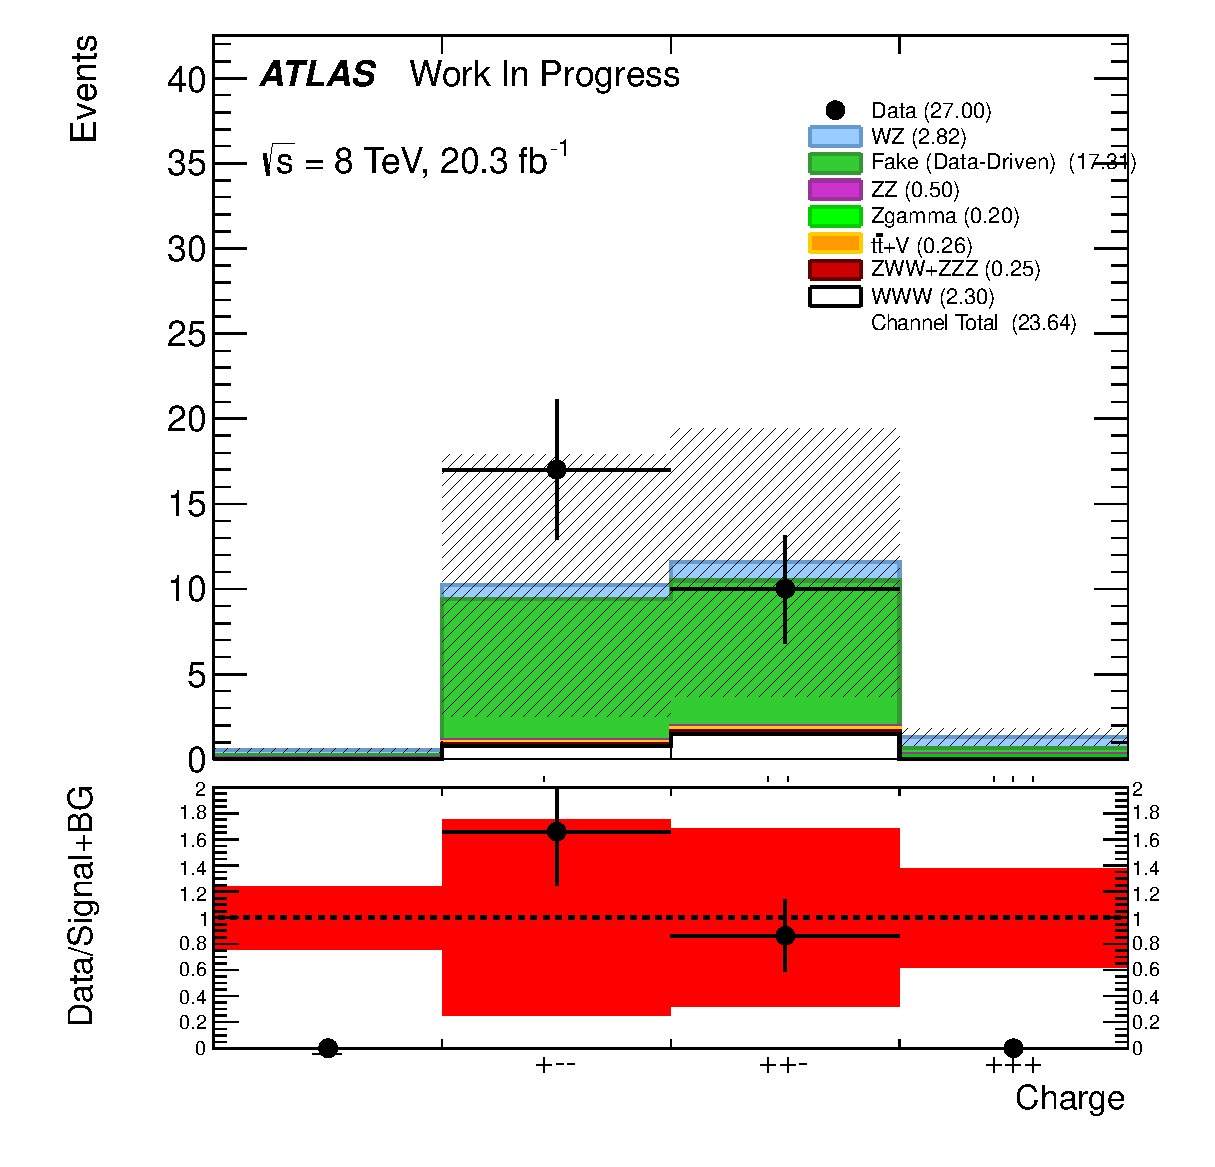
\includegraphics[width=0.3\columnwidth]{figures/appendix_signal_selection/Nov24Update_FakeSys_KFacSys_LinearY_Rebin/output/jobs/MxM/DataFull_Rates_May13_FakeRatesExactly2Loose_MuonMxMBJetGt0_ElBJetGt0SubtractPC_MxM/PreselectionNov23_15_0SFOS_physics/weight_all/eps/TotalCharge_histratio.eps}
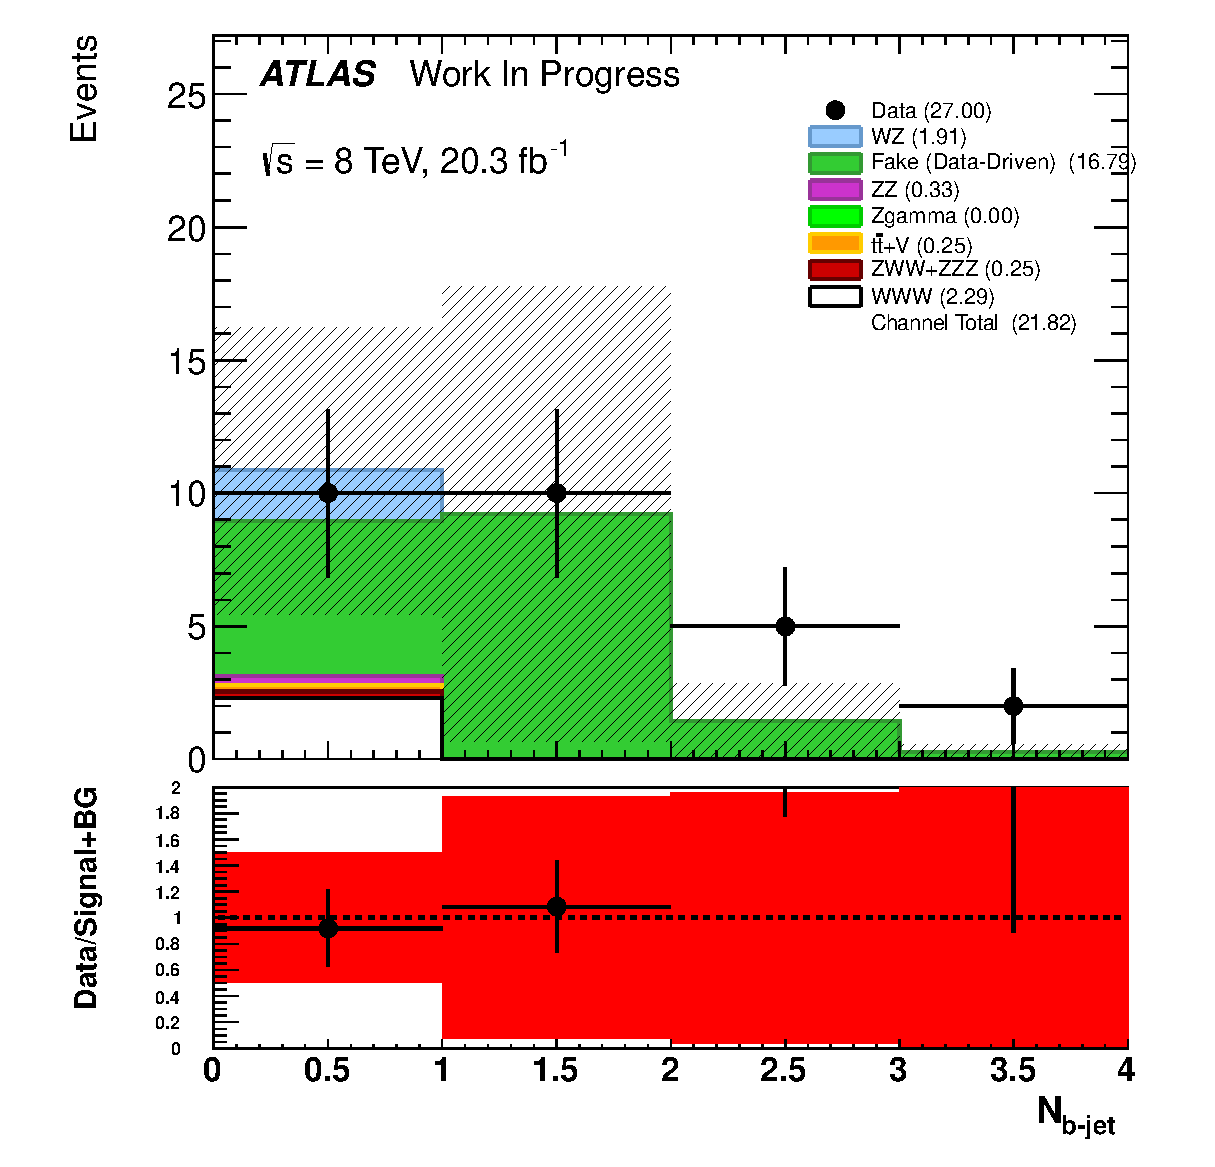
\includegraphics[width=0.3\columnwidth]{figures/appendix_signal_selection/Nov24Update_FakeSys_KFacSys_LinearY_Rebin/output/jobs/MxM/DataFull_Rates_May13_FakeRatesExactly2Loose_MuonMxMBJetGt0_ElBJetGt0SubtractPC_MxM/PreselectionNov23_15_0SFOS_ChargeAbs1_physics/weight_all/eps/NBTaggedJets_histratio.eps}
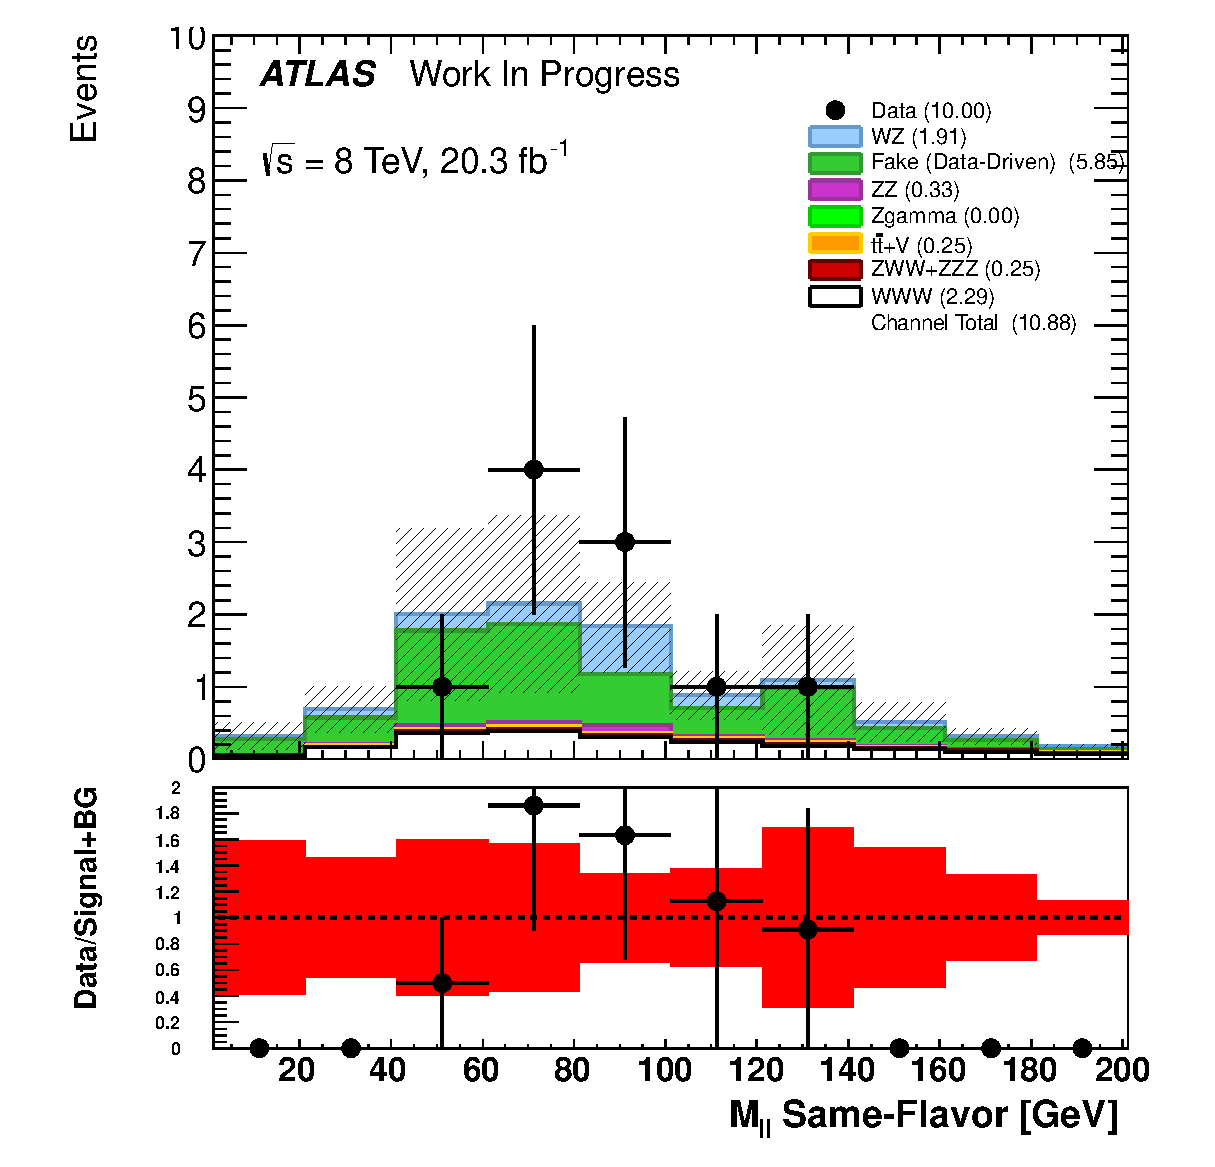
\includegraphics[width=0.3\columnwidth]{figures/appendix_signal_selection/Nov24Update_FakeSys_KFacSys_LinearY_Rebin/output/jobs/MxM/DataFull_Rates_May13_FakeRatesExactly2Loose_MuonMxMBJetGt0_ElBJetGt0SubtractPC_MxM/PreselectionNov23_15_0SFOS_ChargeAbs1_BVeto85_physics/weight_all/eps/InvariantMassSF_histratio.eps}
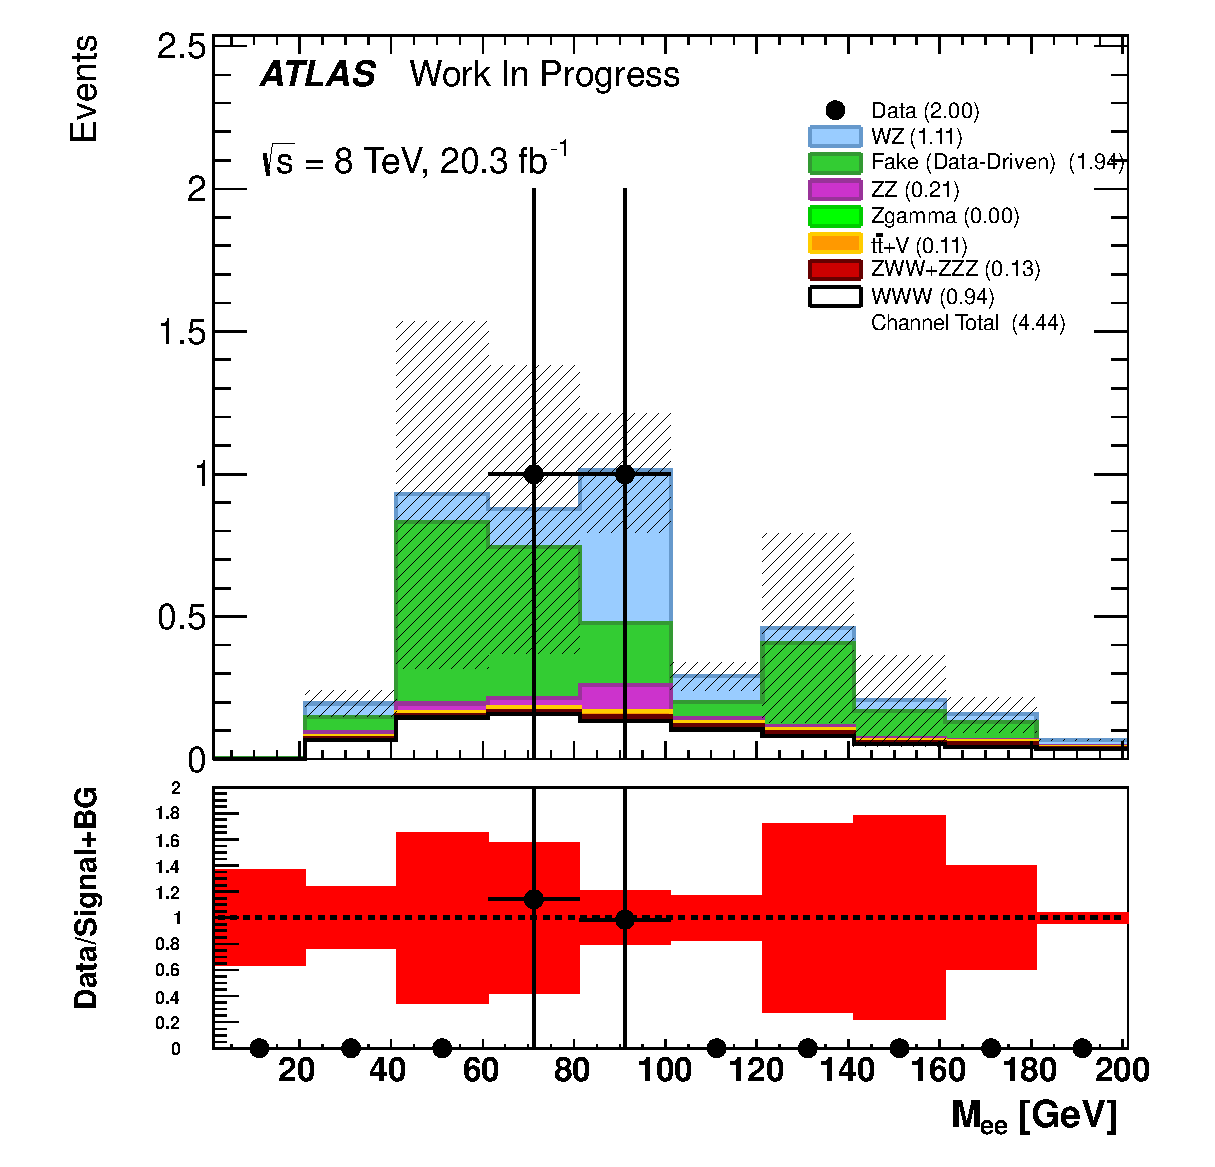
\includegraphics[width=0.3\columnwidth]{figures/appendix_signal_selection/Nov24Update_FakeSys_KFacSys_LinearY_Rebin/output/jobs/MxM/DataFull_Rates_May13_FakeRatesExactly2Loose_MuonMxMBJetGt0_ElBJetGt0SubtractPC_MxM/PreselectionNov23_15_0SFOS_ChargeAbs1_BVeto85_SFMllGt20_physics/weight_all/eps/InvariantMassElEl_histratio.eps}
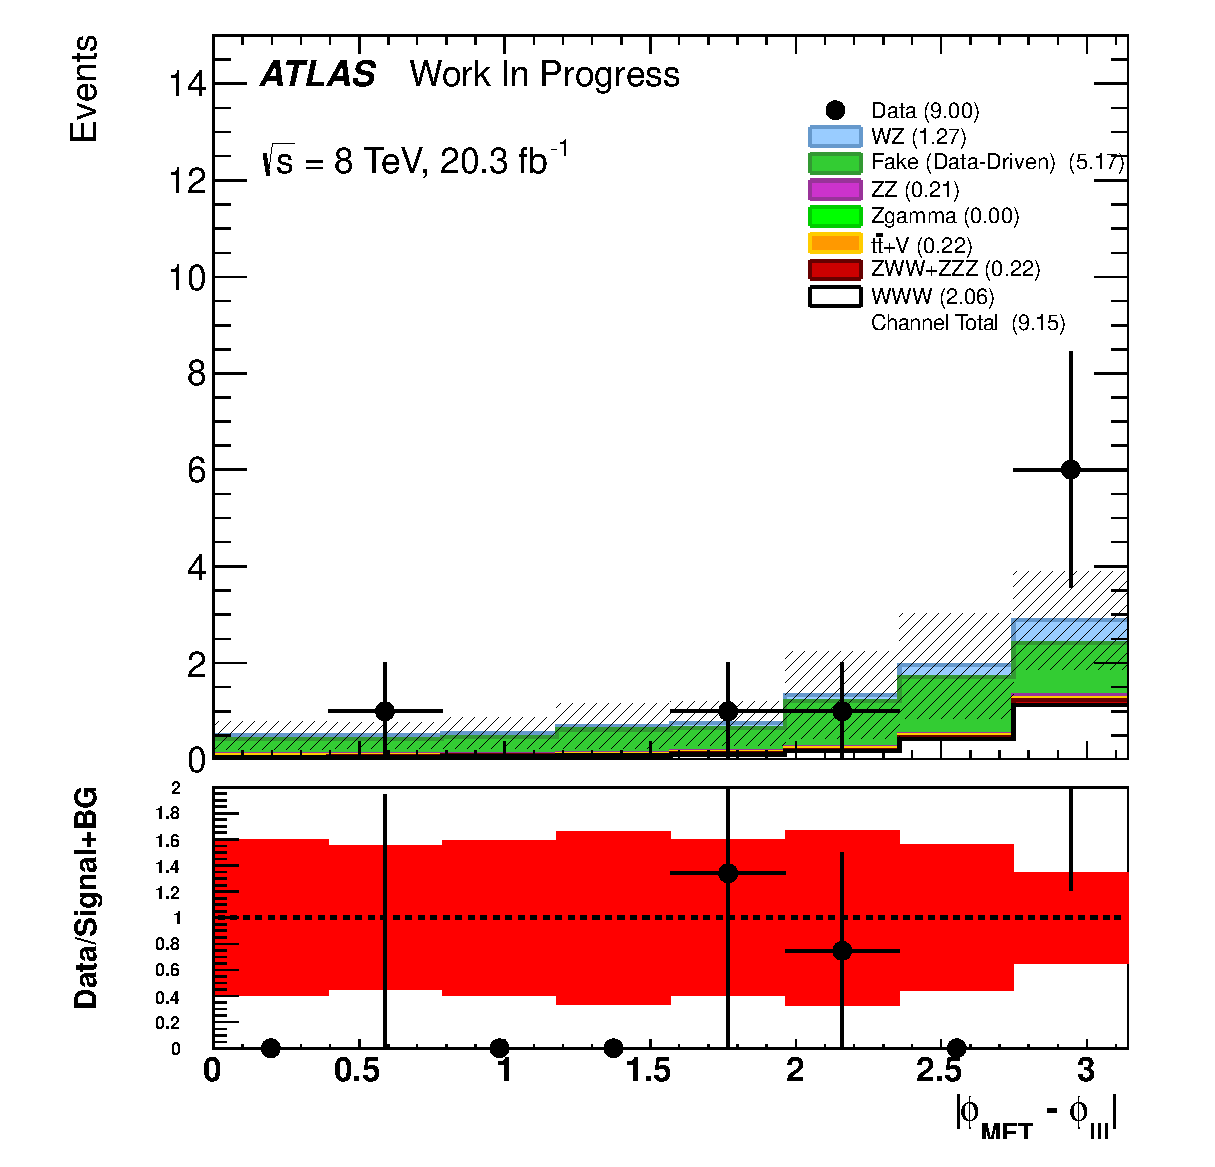
\includegraphics[width=0.3\columnwidth]{figures/appendix_signal_selection/Nov24Update_FakeSys_KFacSys_LinearY_Rebin/output/jobs/MxM/DataFull_Rates_May13_FakeRatesExactly2Loose_MuonMxMBJetGt0_ElBJetGt0SubtractPC_MxM/PreselectionNov23_15_0SFOS_ChargeAbs1_BVeto85_SFMllGt20_SSMeeZVeto15_physics/weight_all/eps/DeltaPhiMET123_Abs_histratio.eps}
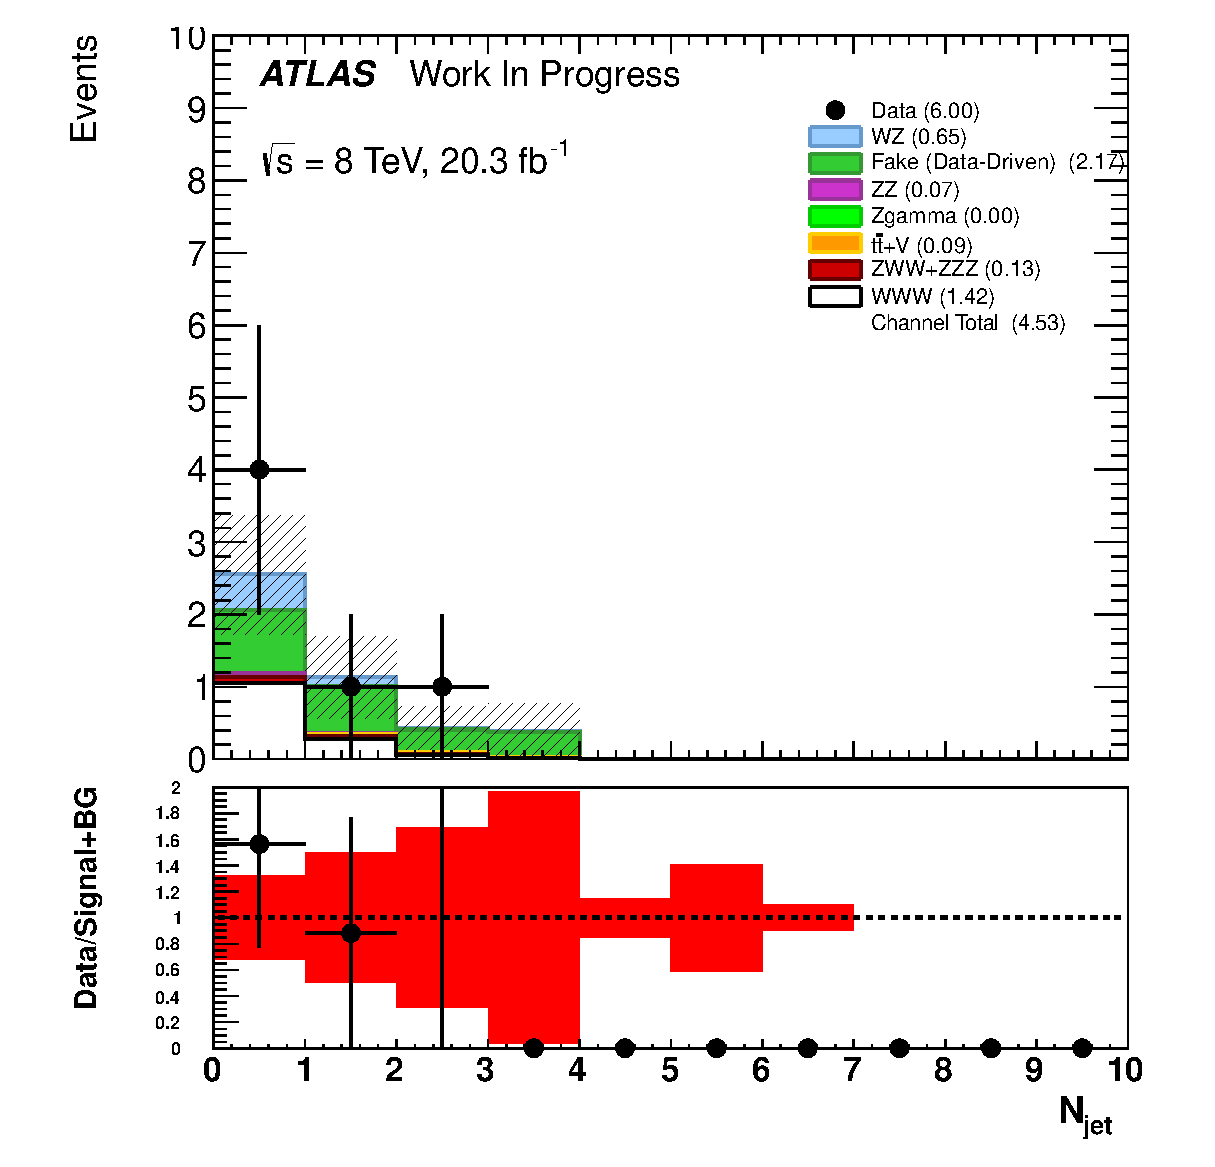
\includegraphics[width=0.3\columnwidth]{figures/appendix_signal_selection/Nov24Update_FakeSys_KFacSys_LinearY_Rebin/output/jobs/MxM/DataFull_Rates_May13_FakeRatesExactly2Loose_MuonMxMBJetGt0_ElBJetGt0SubtractPC_MxM/PreselectionNov23_15_0SFOS_ChargeAbs1_BVeto85_SFMllGt20_SSMeeZVeto15_DeltaPhi2p5_physics/weight_all/eps/NJets_histratio.eps}
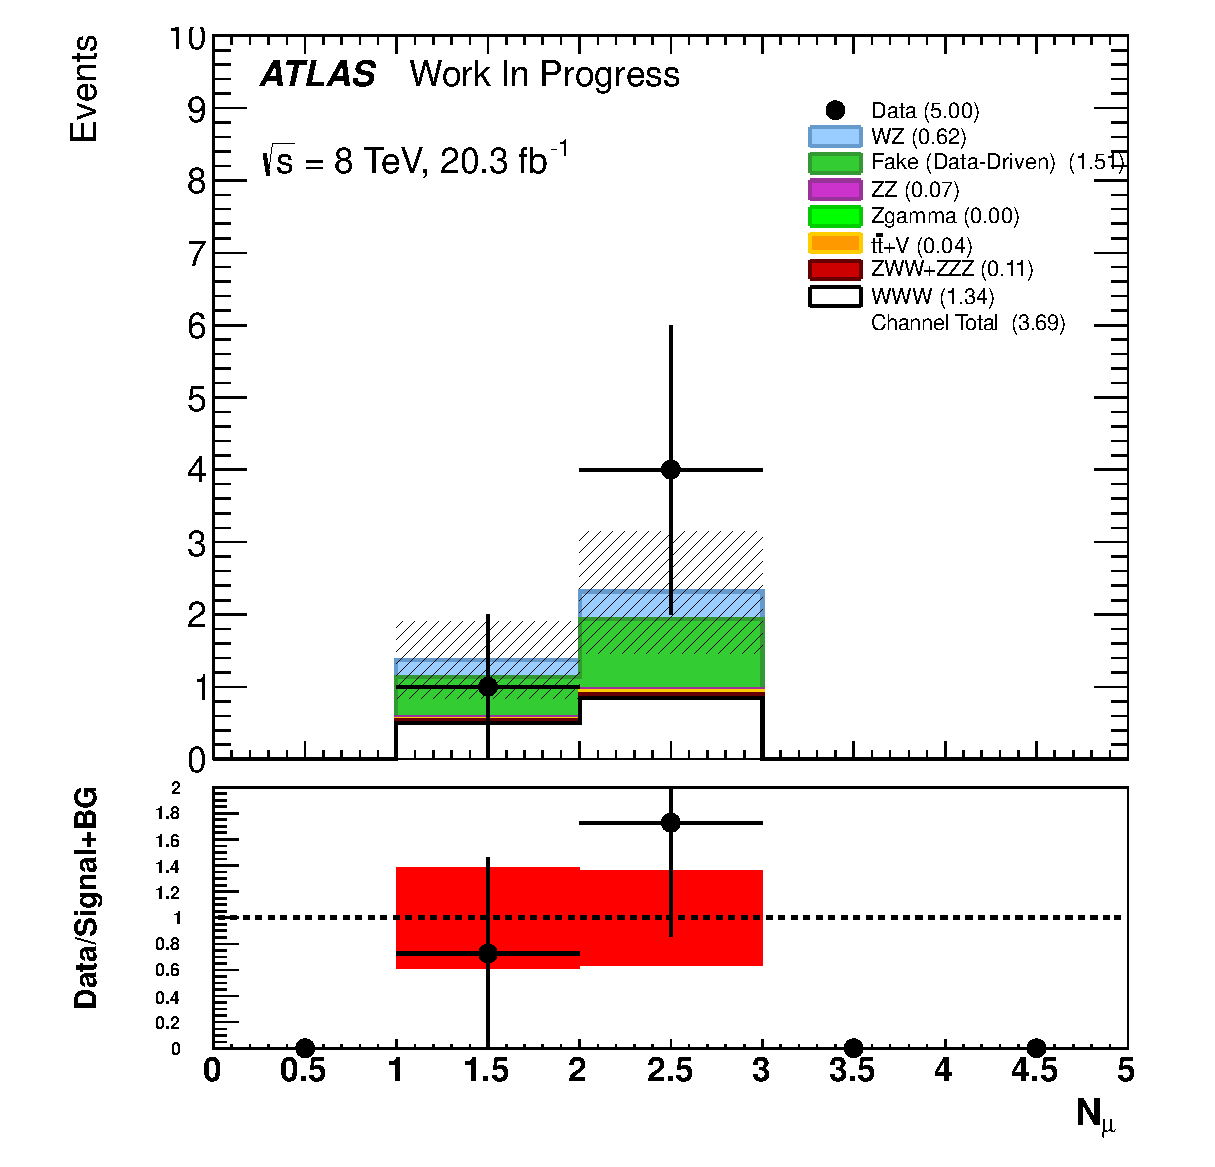
\includegraphics[width=0.3\columnwidth]{figures/appendix_signal_selection/Nov24Update_FakeSys_KFacSys_LinearY_Rebin/output/jobs/MxM/DataFull_Rates_May13_FakeRatesExactly2Loose_MuonMxMBJetGt0_ElBJetGt0SubtractPC_MxM/PreselectionNov23_15_0SFOS_ChargeAbs1_BVeto85_SFMllGt20_SSMeeZVeto15_DeltaPhi2p5_NJetLt2_physics/weight_all/eps/NMuons_histratio.eps}

%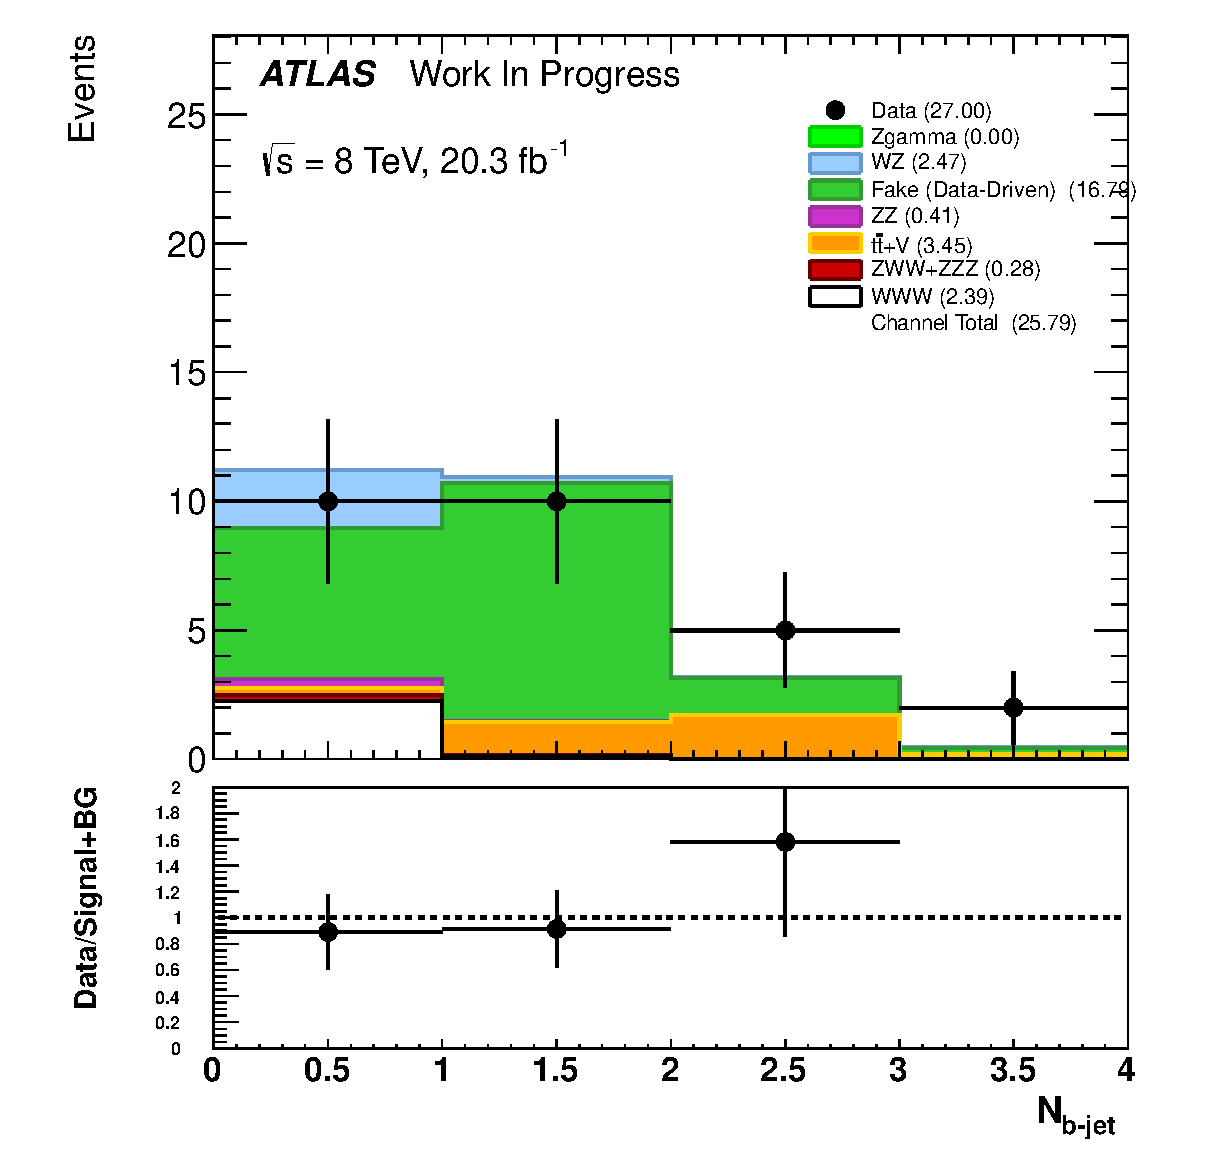
\includegraphics[width=0.3\columnwidth]{figures/appendix_signal_selection/PreselectionJune2_NoSTVF_0SFOS_ChargeAbs1_physics/weight_all/eps/NBTaggedJets_histratio.eps}
%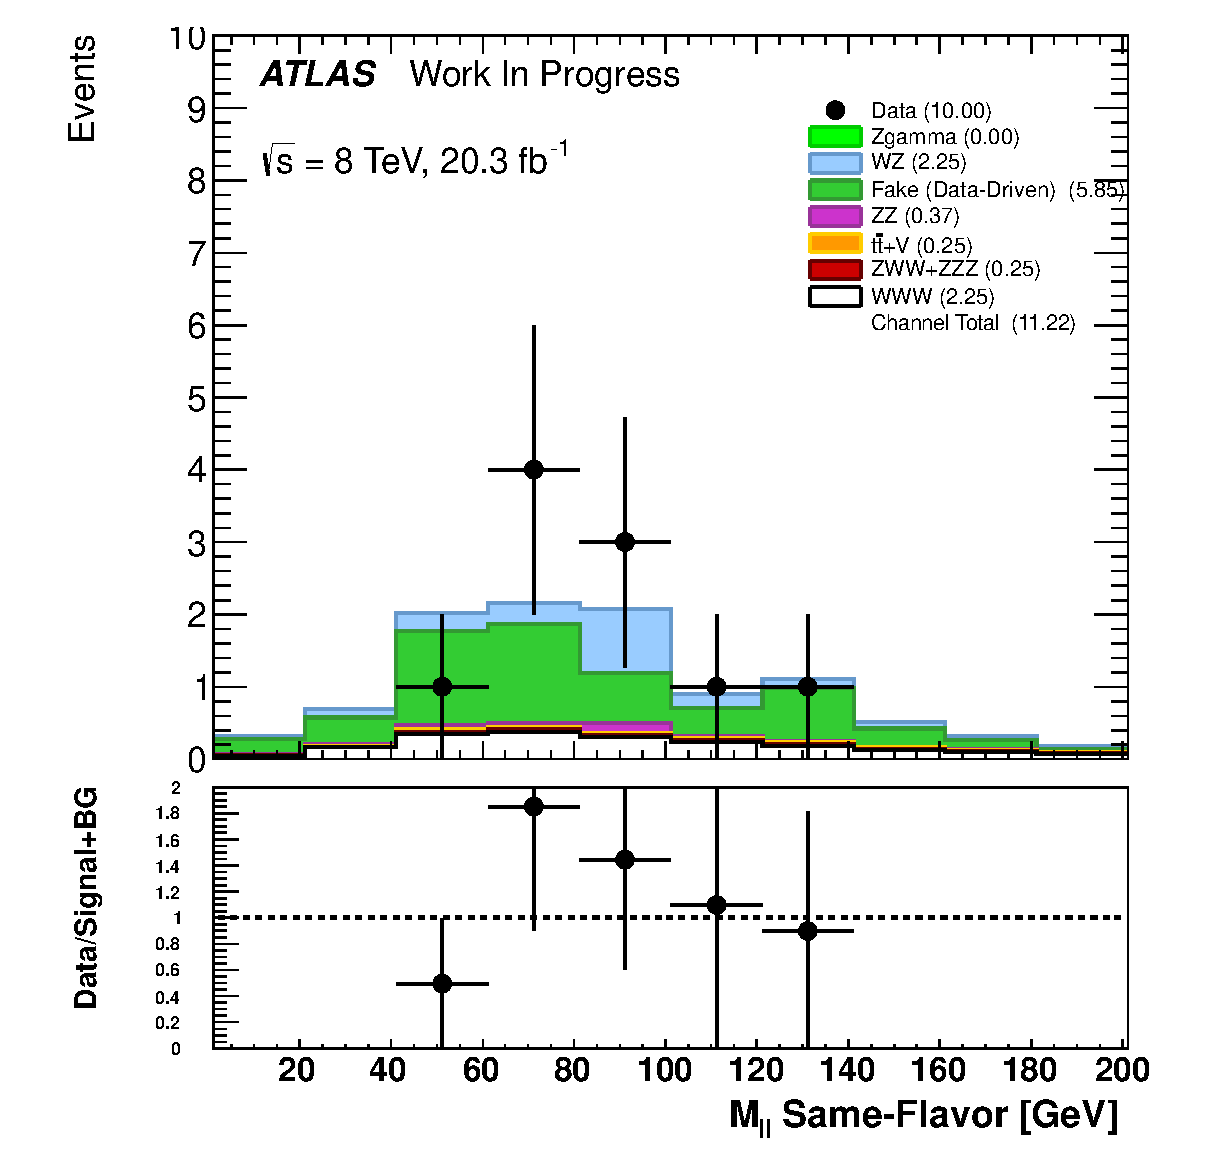
\includegraphics[width=0.3\columnwidth]{figures/appendix_signal_selection/PreselectionJune2_NoSTVF_0SFOS_ChargeAbs1_BVeto85_physics/weight_all/eps/InvariantMassSF_histratio.eps}
%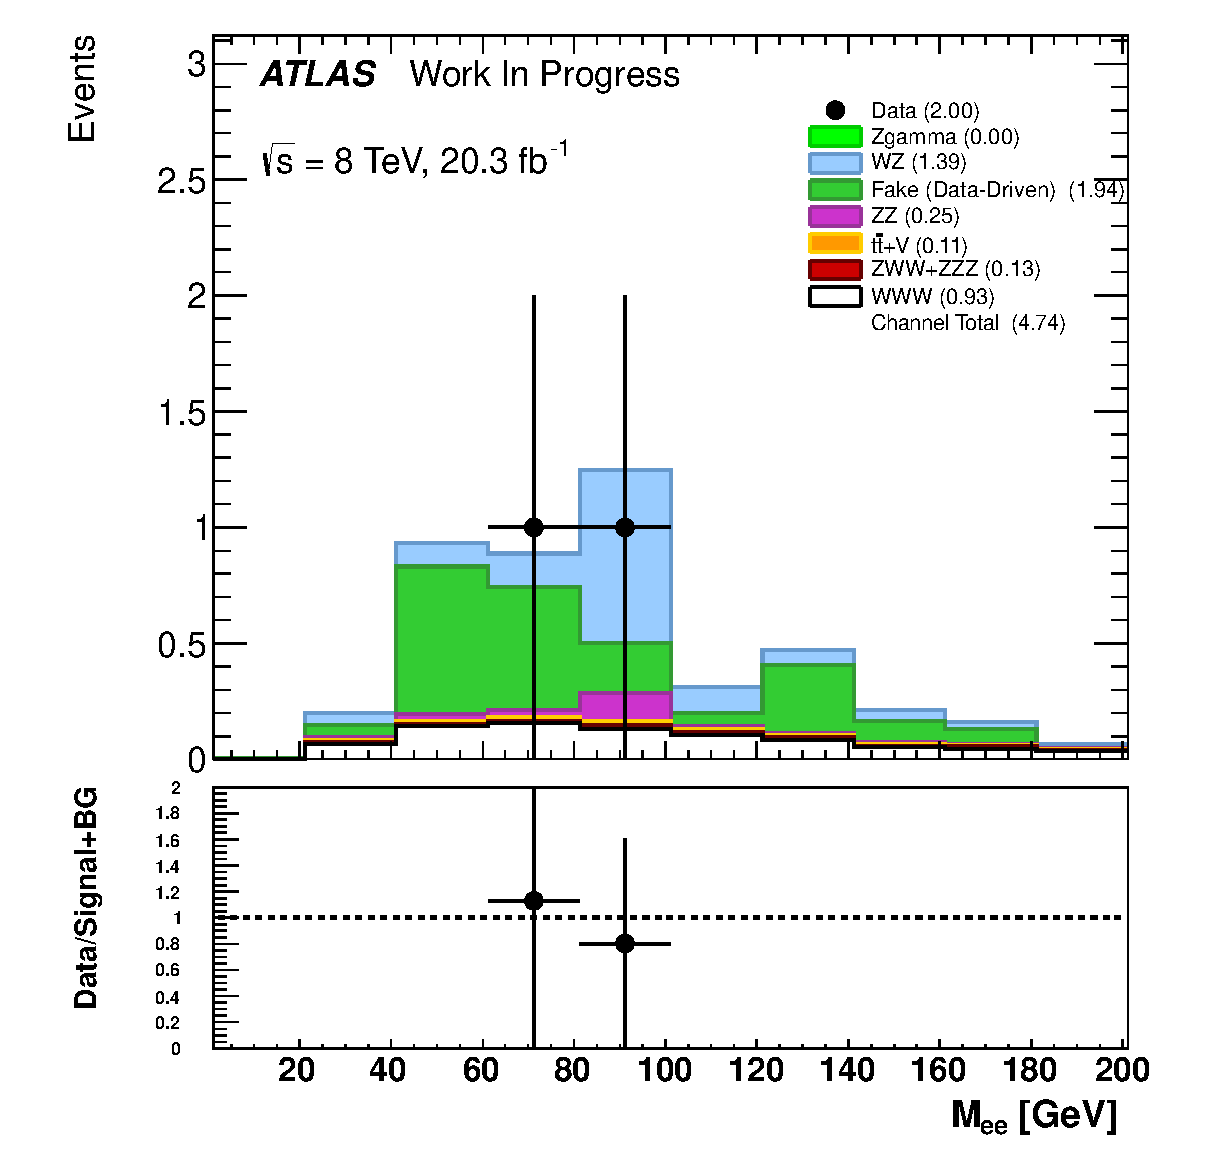
\includegraphics[width=0.3\columnwidth]{figures/appendix_signal_selection/PreselectionJune2_NoSTVF_0SFOS_ChargeAbs1_BVeto85_SFMllGt20_physics/weight_all/eps/InvariantMassElEl_histratio.eps}
%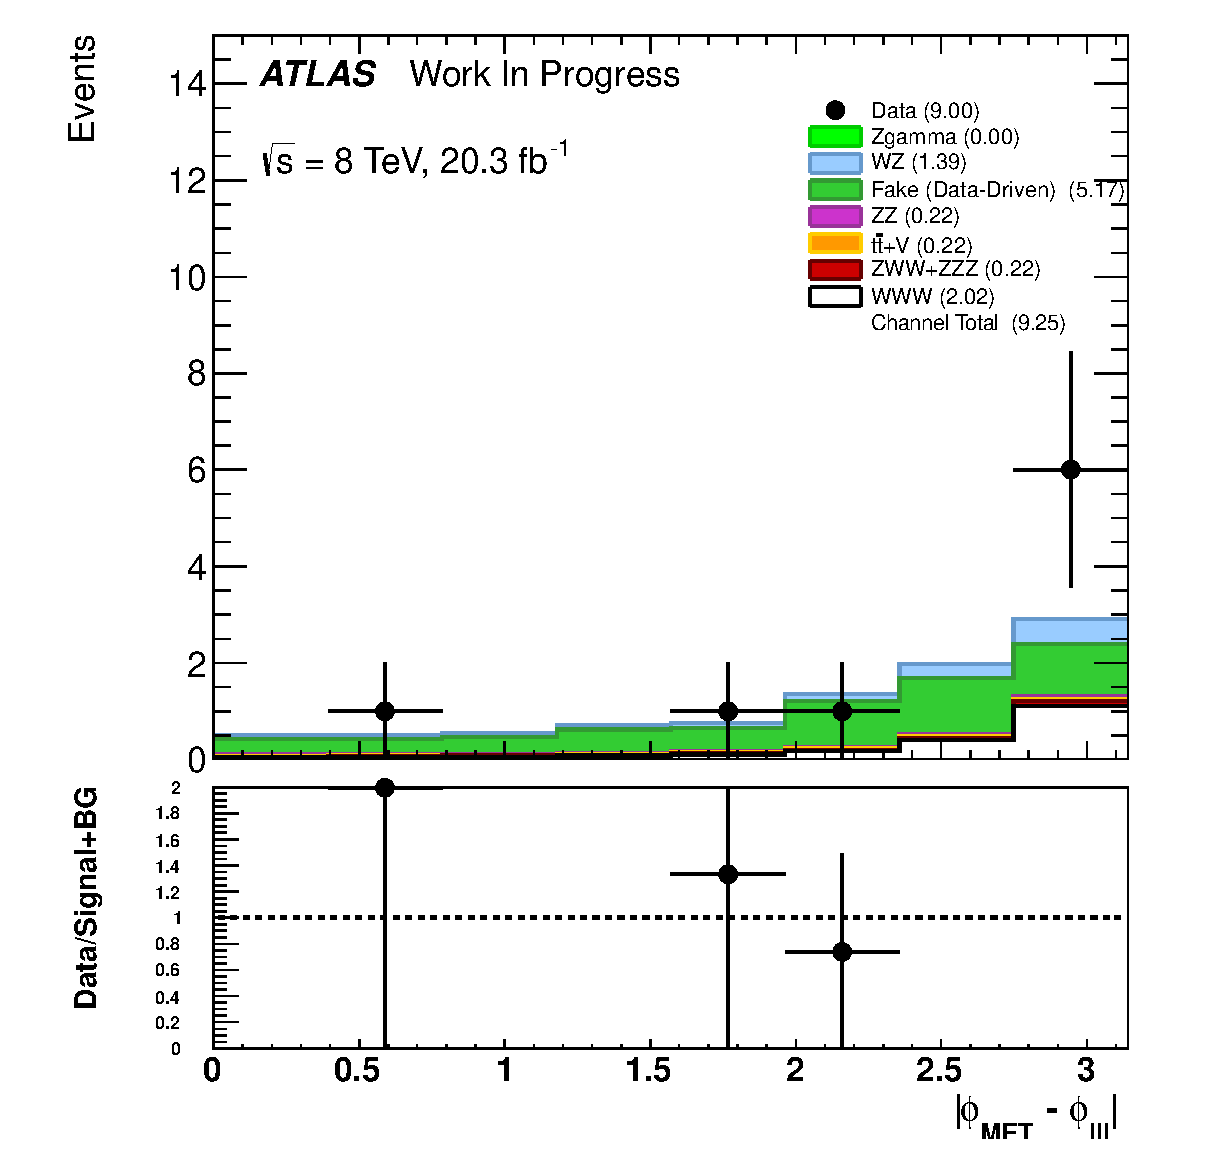
\includegraphics[width=0.3\columnwidth]{figures/appendix_signal_selection/PreselectionJune2_NoSTVF_0SFOS_ChargeAbs1_BVeto85_SFMllGt20_SSMeeZVeto15_physics/weight_all/eps/DeltaPhiMET123_Abs_histratio.eps}
%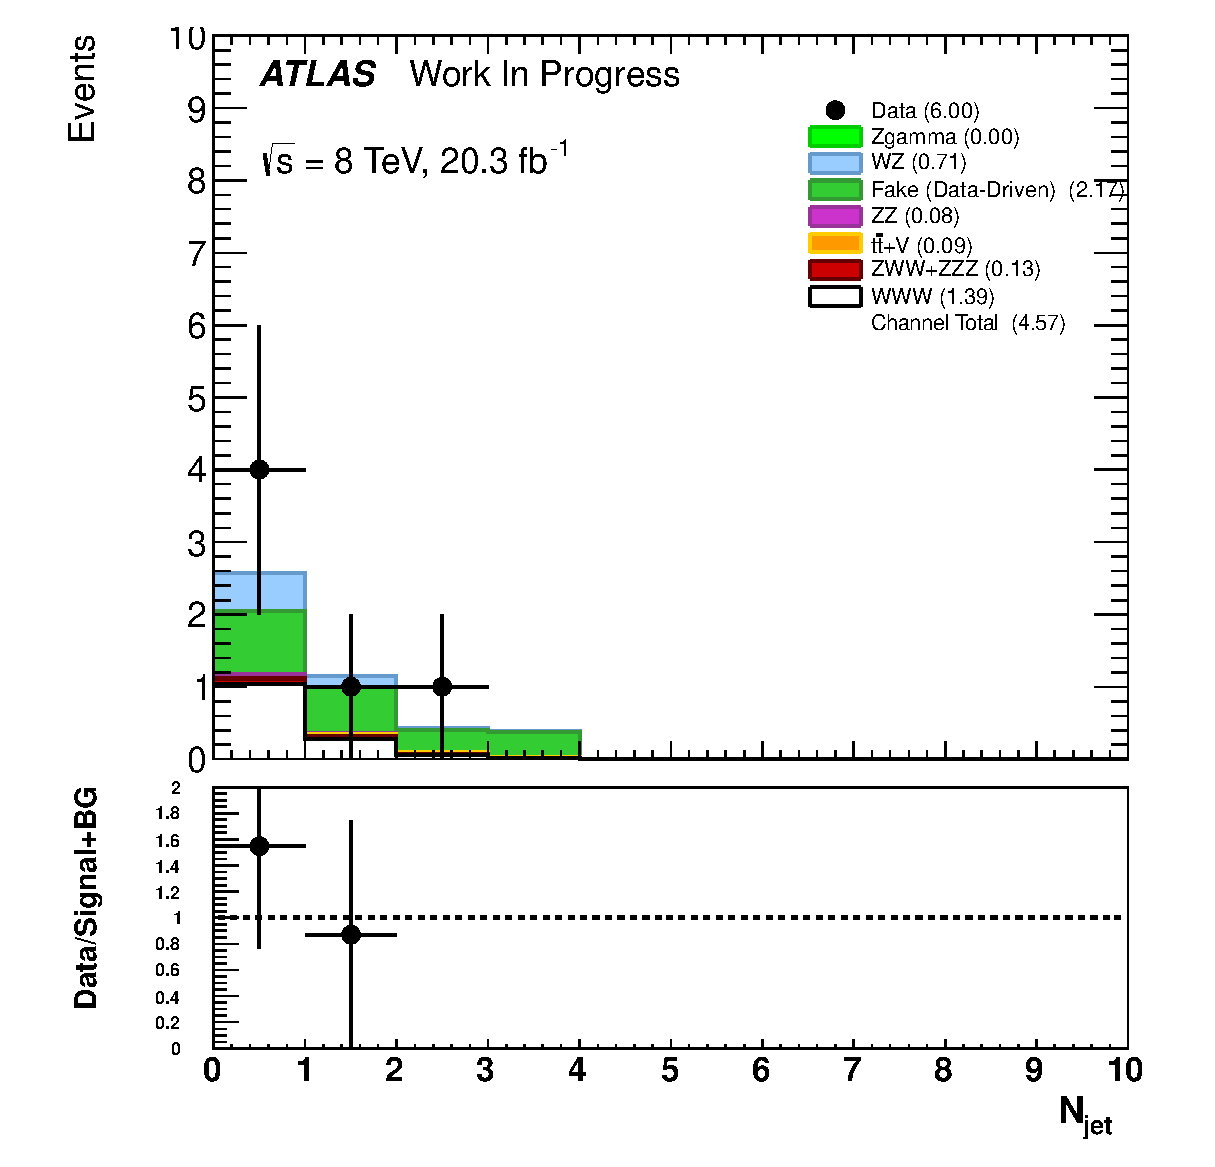
\includegraphics[width=0.3\columnwidth]{figures/appendix_signal_selection/PreselectionJune2_NoSTVF_0SFOS_ChargeAbs1_BVeto85_SFMllGt20_SSMeeZVeto15_DeltaPhi2p5_physics/weight_all/eps/NJets_histratio.eps}
%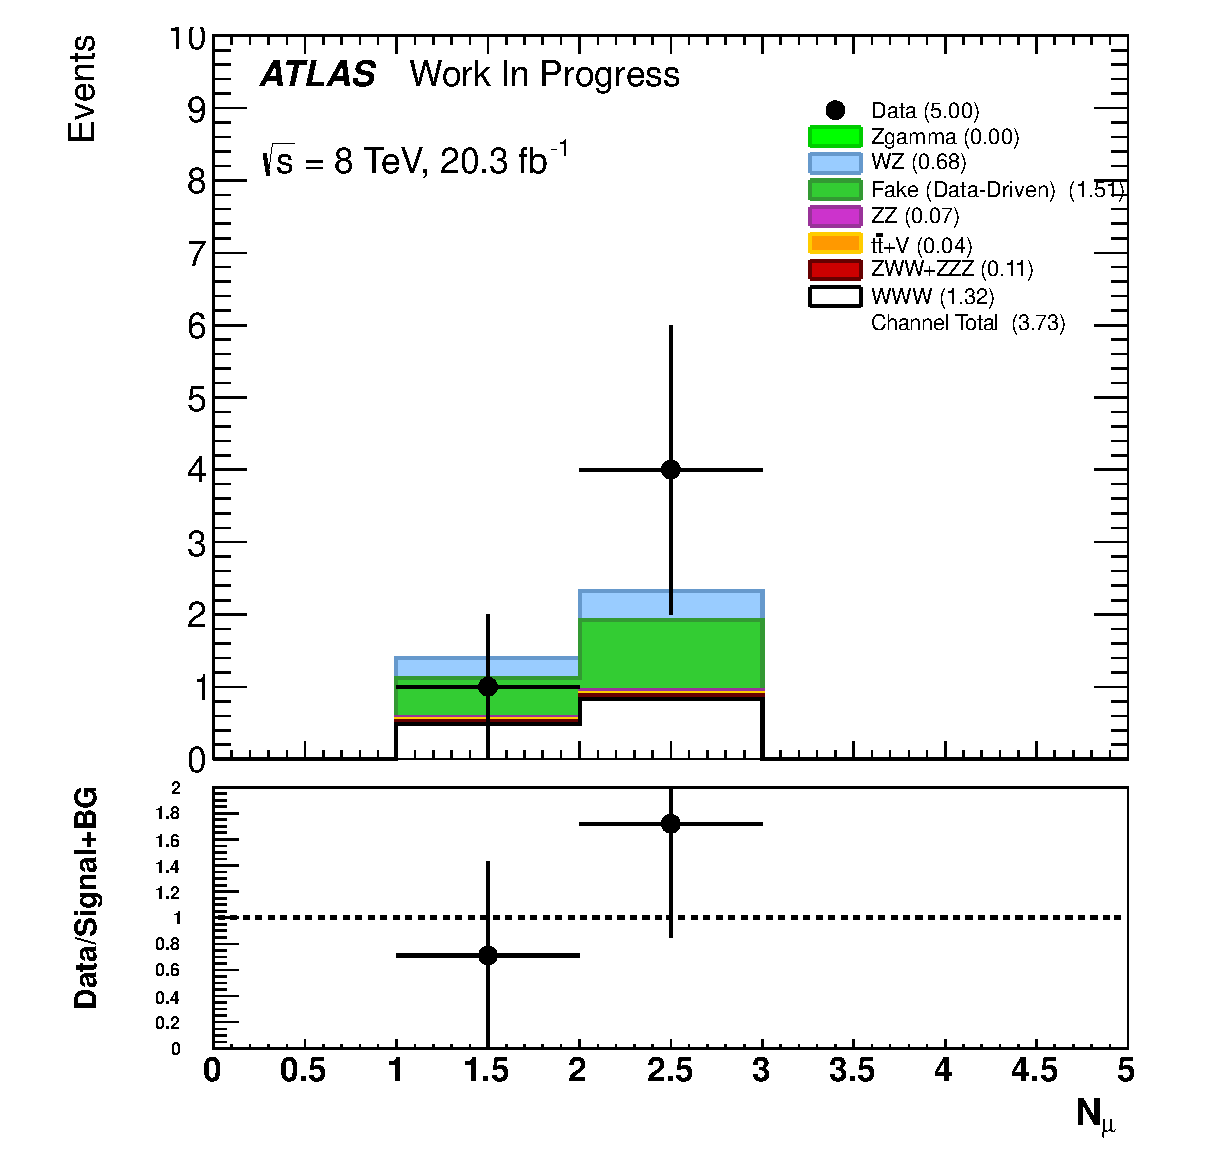
\includegraphics[width=0.3\columnwidth]{figures/appendix_signal_selection/PreselectionJune2_NoSTVF_0SFOS_ChargeAbs1_BVeto85_SFMllGt20_SSMeeZVeto15_DeltaPhi2p5_NJetLt2_physics/weight_all/eps/NMuons_histratio.eps}
\caption{Distributions showing data compared to the signal plus background estimate in the 0 SFOS region at each stage 
of the selection before the cuts are applied to the given distribution. 
Plots should be read sequentially from left to right
and from top to bottom. 
Referring to Table~\ref{tab:cutflow_weighted_0sfos}, the top left
plot is shown before cut \#3 is applied, top middle is before cut \#5, and
so on until the bottom right which is after all cuts are applied.
}
\label{fig:0sfos}
\end{figure}

The prediction from the 0 SFOS signal region at each stage of the selection
is summarized in 
\tab\ref{tab:cutflow_weighted_0sfos}
for the signal and background predictions, as well as for the data.
There is also a more detailed set of predictions at each stage for the 
different background sources in 
\tab\ref{tab:cutflow_weighted_0sfos_bg}. 
From this, we can clearly see the enormous impact of the 0 SFOS
cut on removing the backgrounds, for the $WZ$ background in particular.
We can also see the strong impact that the \nbjet~and \deltaphi~
cuts have without removing much of the signal.
We can also see the signal plus background predictions as 
compared to the data
for the distribution just before each cut is applied in 
\fig\ref{fig:0sfos}. From this we can clearly see
that the data seems to be well modeled at each stage of the selection.

After the full selection is applied,
the 0 SFOS signal region is found to be the most sensitive of the three
channels, as expected, with a predicted signal to background ratio of 56\%.
This can be seen from \tab\ref{tab:sys_summary}, where the expected signal
is 1.344 compared to an expected background of 2.35. Together they 
combine to give a total prediction of 3.69 signal plus background events. 
The Poisson probability of observing $\leq 5$ events with 3.69 events expected 
from the signal plus background prediction is 30.7\%. 
Thus, we can see that this is in good agreement with the observed 5 events in data
from the statistical uncertainty alone. 

The fake background makes up more than half of the total expected background
prediction, with 1.51 background events predicted from fakes compared to 
2.35 events expected from the total background.  The systematic
uncertainty on the fake background is approaching 100\%.
As can be seen in \tab\ref{tab:sys_breakdown}, this results in the
systematic uncertainty on the total background estimate 
that is approaching 60\%, or roughly the size of the fake
background contribution.
This further increases the compatibility 
of the data with the expectation, but also reduces the sensitivity.

The other backgrounds are less important. The $WZ$ background
is the second largest, coming from charge mis-identification, 
with $0.6176$ events predicted. The uncertainty on the $WZ$
background is dominated by that from the $WZ$ normalization uncertainty,
which is 10\%, and also has a small contribution from the 
charge mis-identification estimate uncertainty.
The $VVV$ contributions is the third largest, predicting 0.1126
with a small uncertainty.
The $ZZ$ background has a similar source and 
uncertainty as the $WZ$, but is about 10 times
smaller in size. The $\ttV$ background contributes even less
and the DPS and $Z\gamma$ backgrounds have
0 contribution within the statistical uncertainties of the MC.



\subsubsection{1 SFOS Signal Region}

\begin{table}[ht!]
\small
\centering
\begin{tabular}{l||c|c||c|c||c|c}
\hline
 &                 \multicolumn{2}{c||}{Signal}            &  \multicolumn{2}{c||}{Background} &  \multicolumn{2}{c}{Data} \\
   & Yield & Eff. & Yield & Eff. & Yield & Eff.\\
   \hline\hline
   %1. Pre-selection &  $9.78$ & --- &  $2388.48$ & --- & $2472$ &  --- \\
   %\hline
   1. 1 SFOS &  $4.67$ &  --- &  $1231.49$ &  --- & $1260$ &  --- \\ 
   \hline
   2. $N_{\mathrm{b-jet}} = 0$ &  $4.42$ &  $0.94$ &  $1086.66$ &  $0.88$ & $1095$ &  $0.87$\\ 
   \hline
   3. NOT $m_Z - 35~\mathrm{GeV} <$  &  \multirow{2}{*}{$2.76$} &  \multirow{2}{*}{$0.63$} &  \multirow{2}{*}{$97.96$} &  \multirow{2}{*}{$0.090$} & \multirow{2}{*}{$93$} &  \multirow{2}{*}{$0.08$}\\ 
    \hfill$ m_{\mathrm{SFOS}} < m_Z + 20~\mathrm{GeV}$  & & & & &  & \\
   \hline
   4. $E_{T}^{Miss} > 45$ GeV &  $1.91$ &  $0.69$ &  $29.83$ &  $0.30$ & $27$ &  $0.29$\\ 
   \hline
   5. $|\Delta\phi(3l,E_{T}^{Miss})| > 2.5$ &  $1.48$ &  $0.77$ &  $16.73$ &  $0.56$ & $16$ &  $0.59$\\ 
   \hline
   6. $N_{\mathrm{Jet}} \leq 1$ &  $1.39$ &  $0.94$ &  $14.77$ &  $0.88$ & $13$ &  $0.81$\\ 
   \hline
   \end{tabular}

\caption{Cut-flows showing the event yields and efficiencies for each cut in the 1 SFOS signal region
starting from event pre-selection separately for the total signal and total background predictions, along with the observed by data. 
Event yields for MC backgrounds and signal include all weights and are normalized to an integrated luminosity of $20.3~\mathrm{fb}^{-1}$.  
The fake lepton background only includes the matrix method weights.  The data is unweighted.
Efficiencies show the ratio of the yield with respect
to the previous cut.  The efficiency is first calculated at the first cut after event pre-selection.  }
\label{tab:cutflow_weighted_1sfos}
\end{table}

\begin{table}[ht!]
\small
\centering
\begin{tabular}{l||c|c||c|c||c|c}
\hline
 &       \multicolumn{6}{c}{Background}\\
 &  \multicolumn{2}{c||}{$WZ$} & \multicolumn{2}{c||}{$ZZ$} & \multicolumn{2}{c}{$t\bar{t}+V$} \\ 
 & Yield & Eff. & Yield & Eff. & Yield & Eff. \\
\hline\hline
Pre-selection & $1566.91$ & --- &  $323.60$ & --- &  $36.93$ & ---  \\
\hline
1. 1 SFOS &  $757.38$ &  $0.48$ &  $171.39$ &  $0.53$ &  $18.10$ &  $0.49$ \\ 
\hline
2. $N_{\mathrm{b-jet}} = 0$ &  $696.90$ &  $0.92$ &  $150.14$ &  $0.88$ &  $1.42$ &  $0.08$\\ 
\hline
3. NOT $m_Z - 35~\mathrm{GeV} <$  &  \multirow{2}{*}{$44.30$} &  \multirow{2}{*}{$0.06$} &  \multirow{2}{*}{$13.79$} &  \multirow{2}{*}{$0.09$} &  \multirow{2}{*}{$0.37$} &  \multirow{2}{*}{$0.26$} \\ 
\hfill $ m_{\mathrm{SFOS}} < m_Z + 20~\mathrm{GeV}$ & & & &  & & \\
\hline
4. $E_{T}^{Miss} > 45$ GeV &  $21.38$ &  $0.48$ &  $1.46$ &  $0.11$ &  $0.29$ &  $0.78$ \\ 
\hline
5. $|\Delta\phi(3l,E_{T}^{Miss})| > 2.5$ &  $13.07$ &  $0.61$ &  $0.71$ &  $0.49$ &  $0.11$ &  $0.39$ \\ 
\hline
6. $N_{\mathrm{Jet}} \leq 1$ &  $11.90$ &  $0.91$ &  $0.58$ &  $0.82$ &  $0.05$ &  $0.45$ \\ 
\hline
\end{tabular}

\begin{tabular}{l||c|c||c|c||c|c}
\hline
 &       \multicolumn{6}{c}{Background}\\
 &  \multicolumn{2}{c||}{$ZZZ+ZWW$} & \multicolumn{2}{c||}{$Z\gamma$} & \multicolumn{2}{c}{Fake} \\ 
 & Yield & Eff. & Yield & Eff. & Yield & Eff. \\
\hline\hline
%1. Pre-selection &  $3.12$ & --- &  $219.80$ & --- &  $238.12$ & ---  \\
%\hline
1 SFOS &  $1.55$ &  --- &  $149.60$ &  --- &  $133.47$ &  --- \\ 
\hline
$N_{\mathrm{b-jet}} = 0$ &  $1.31$ &  $0.84$ &  $136.96$ &  $0.92$ &  $99.93$ &  $0.75$ \\ 
\hline
NOT $m_Z - 35~\mathrm{GeV} <$  &  \multirow{2}{*}{$0.34$} &  \multirow{2}{*}{$0.26$} &  \multirow{2}{*}{$22.44$} &  \multirow{2}{*}{$0.16$} &  \multirow{2}{*}{$16.72$} &  \multirow{2}{*}{$0.17$} \\ 
$ m_{\mathrm{SFOS}} < m_Z + 20~\mathrm{GeV}$ & & & & & &  \\
\hline
$E_{T}^{Miss} > 45$ GeV &  $0.24$ &  $0.71$ &  $1.36$ &  $0.06$ &  $5.10$ &  $0.31$ \\ 
\hline
$|\Delta\phi(3l,E_{T}^{Miss})| > 2.5$ &  $0.17$ &  $0.69$ &  $0.20$ &  $0.15$ &  $2.47$ &  $0.48$ \\ 
\hline
$N_{\mathrm{Jet}} \leq 1$ &  $0.14$ &  $0.84$ &  $0.20$ &  $1.00$ &  $1.90$ &  $0.77$\\ 
\hline
\end{tabular}

\caption{Cut-flows showing the event yields and efficiencies for each cut in the 1 SFOS signal region
starting from event pre-selection and binned by background category. 
Event yields for MC backgrounds and signal include all weights and are normalized to an integrated luminosity of $20.3~\mathrm{fb}^{-1}$.  
The fake lepton background only includes the matrix method weights.  The data is unweighted.
Efficiencies show the ratio of the yield with respect
to the previous cut.  The efficiency is first calculated at the first cut after event pre-selection.  }
\label{tab:cutflow_weighted_1sfos_bg}
\end{table}


%1 SFOS consolidated
\begin{figure}[ht!]
\centering
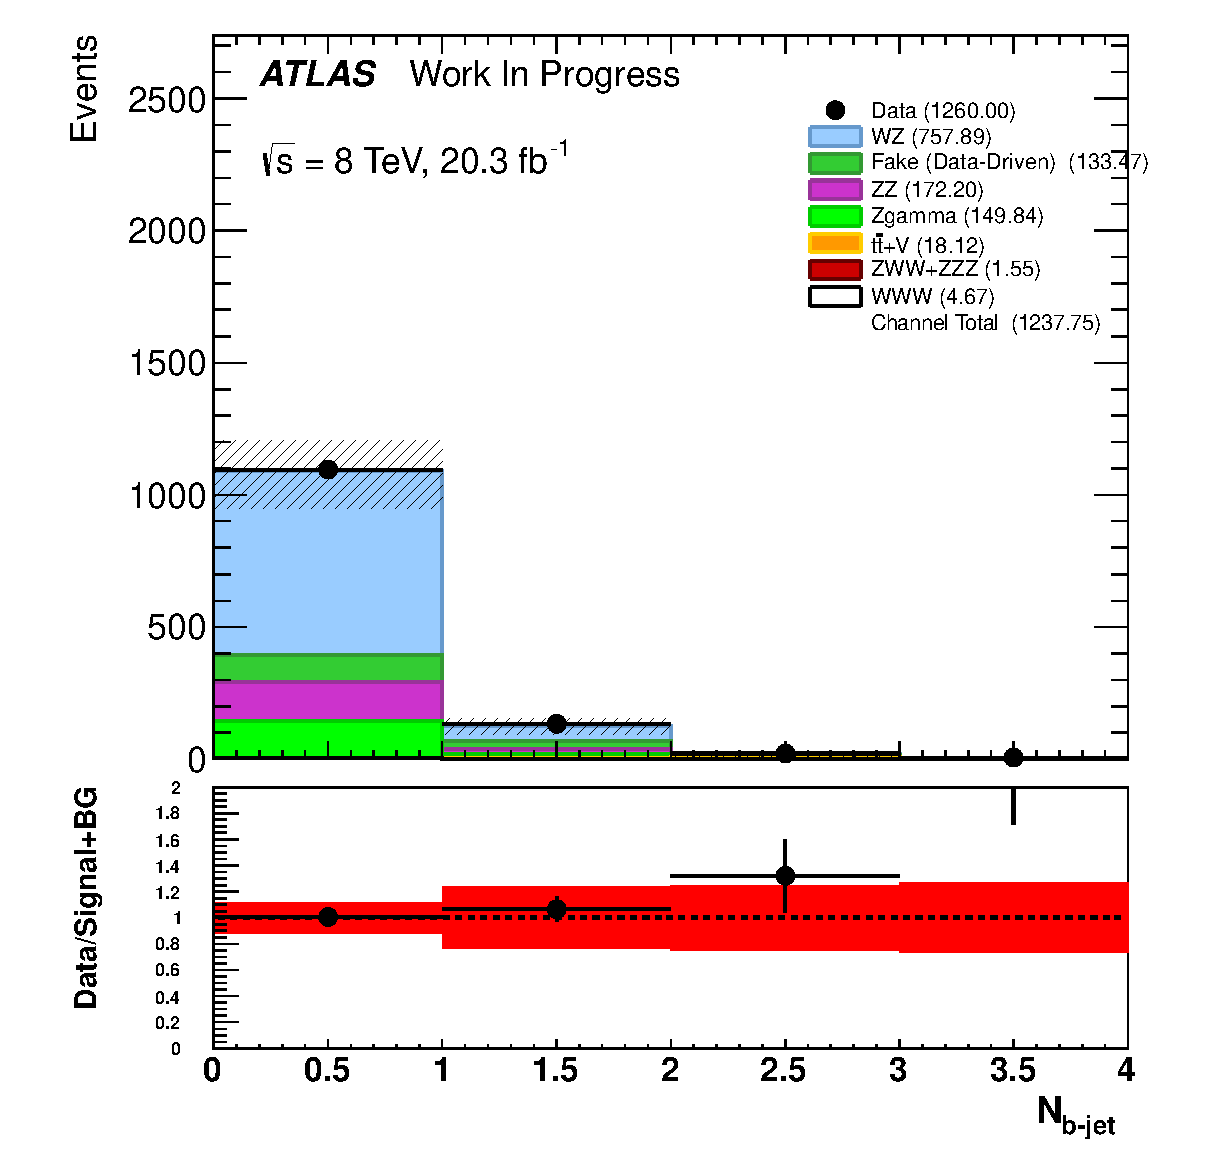
\includegraphics[width=0.3\columnwidth]{figures/appendix_signal_selection/Nov24Update_FakeSys_KFacSys_LinearY_Rebin/output/jobs/MxM/DataFull_Rates_May13_FakeRatesExactly2Loose_MuonMxMBJetGt0_ElBJetGt0SubtractPC_MxM/PreselectionNov23_15_1SFOS_ChargeAbs1_physics/weight_all/eps/NBTaggedJets_histratio.eps}
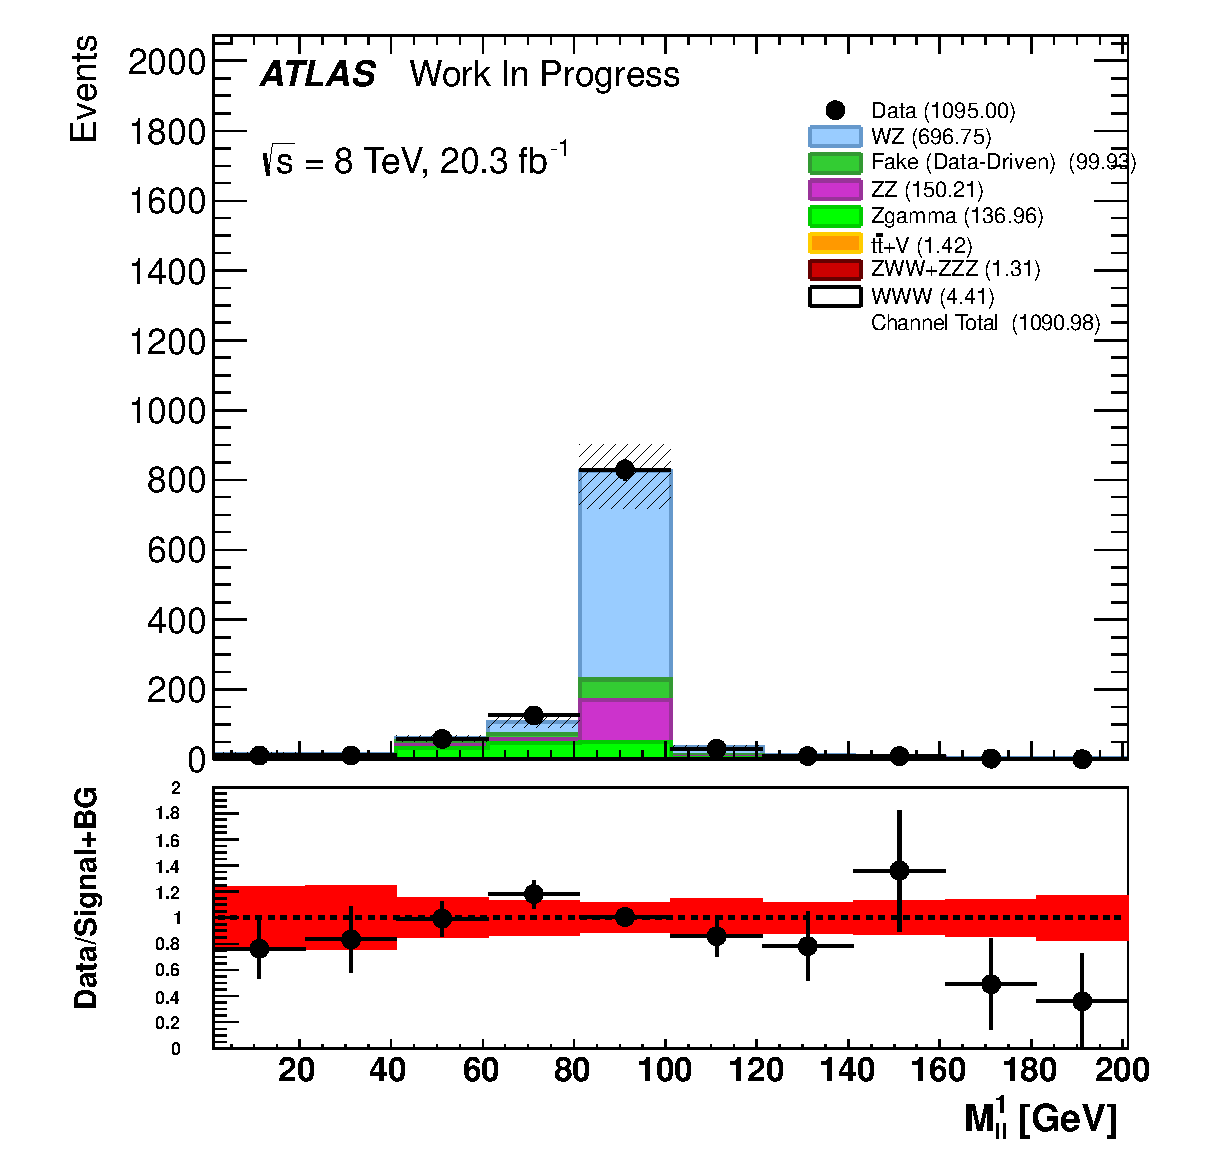
\includegraphics[width=0.3\columnwidth]{figures/appendix_signal_selection/Nov24Update_FakeSys_KFacSys_LinearY_Rebin/output/jobs/MxM/DataFull_Rates_May13_FakeRatesExactly2Loose_MuonMxMBJetGt0_ElBJetGt0SubtractPC_MxM/PreselectionNov23_15_1SFOS_ChargeAbs1_BVeto85_physics/weight_all/eps/InvariantMassSFOS_histratio.eps}
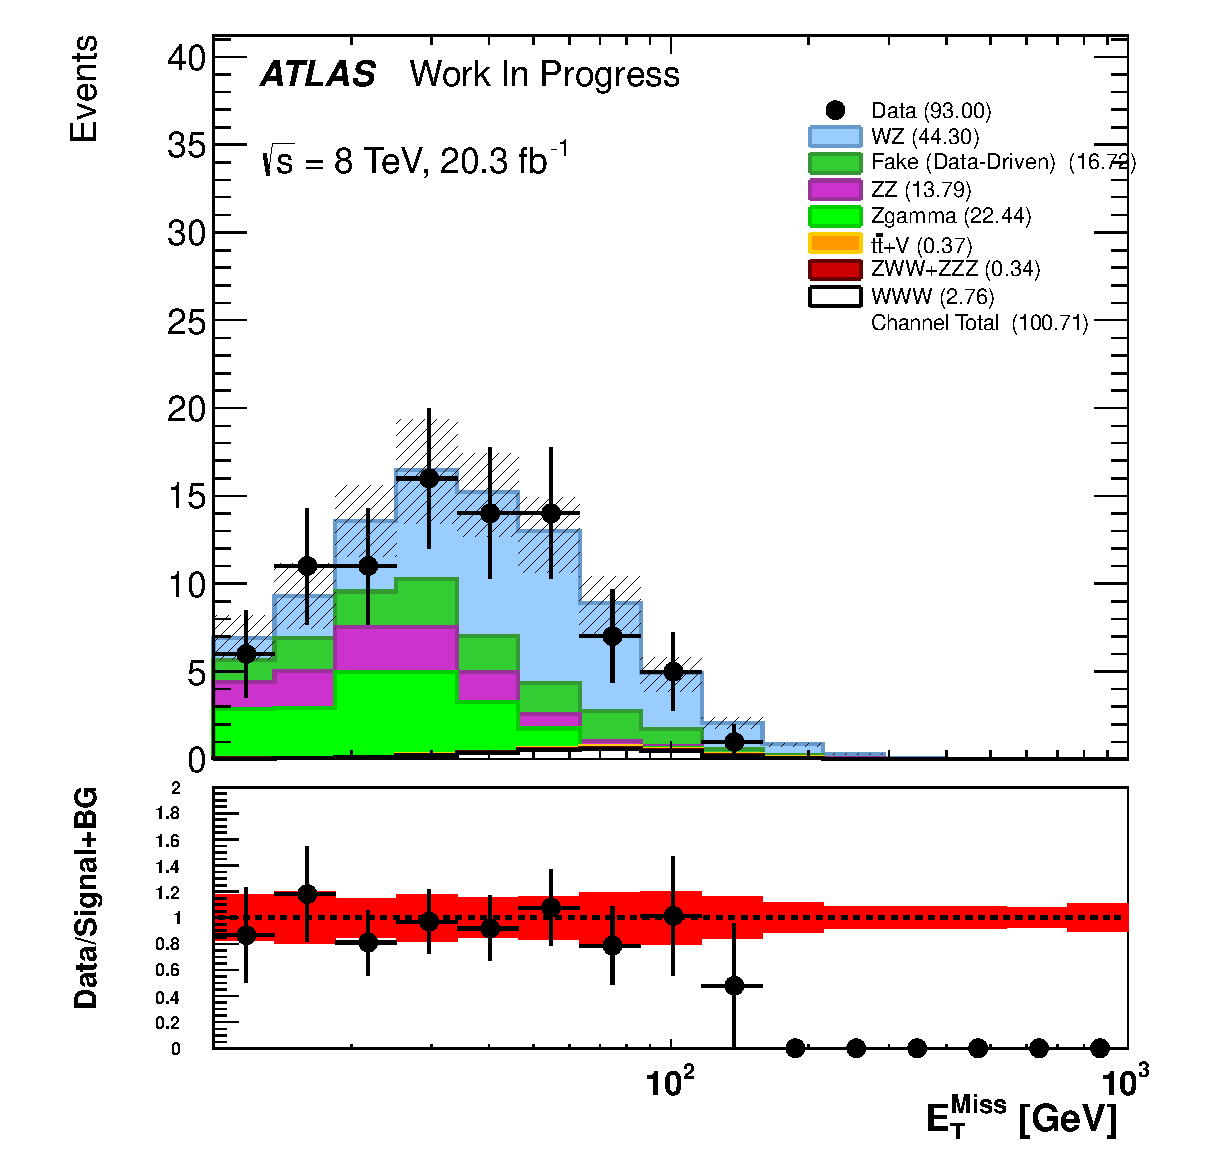
\includegraphics[width=0.3\columnwidth]{figures/appendix_signal_selection/Nov24Update_FakeSys_KFacSys_LinearY_Rebin/output/jobs/MxM/DataFull_Rates_May13_FakeRatesExactly2Loose_MuonMxMBJetGt0_ElBJetGt0SubtractPC_MxM/PreselectionNov23_15_1SFOS_ChargeAbs1_BVeto85_ZVetoLow35High25GeV_physics/weight_all/eps/MET_Et_histratio.eps}
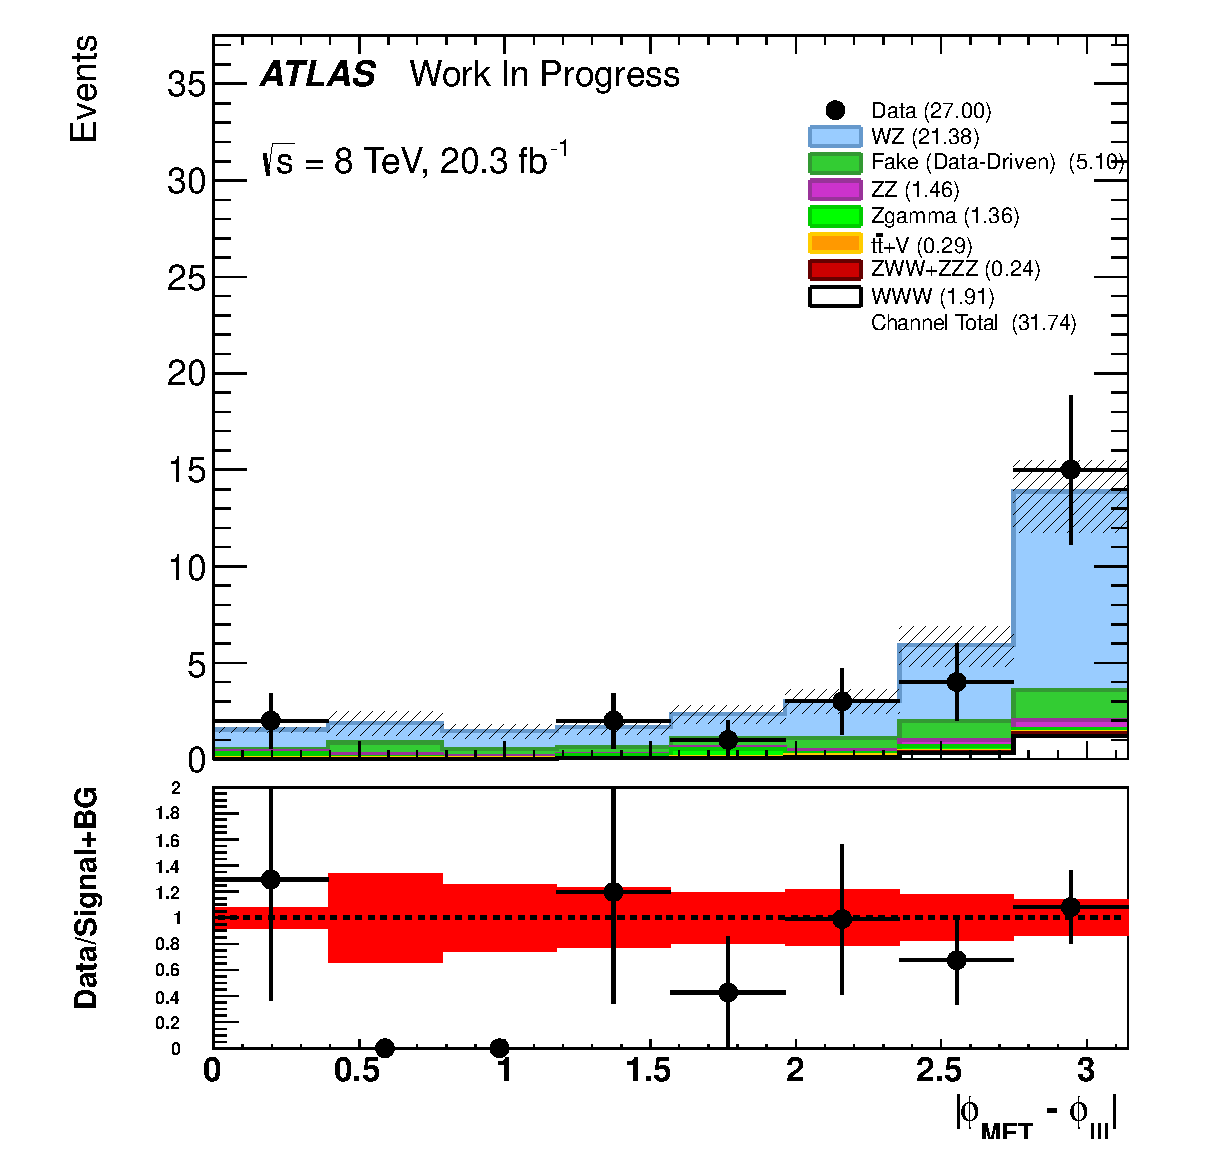
\includegraphics[width=0.3\columnwidth]{figures/appendix_signal_selection/Nov24Update_FakeSys_KFacSys_LinearY_Rebin/output/jobs/MxM/DataFull_Rates_May13_FakeRatesExactly2Loose_MuonMxMBJetGt0_ElBJetGt0SubtractPC_MxM/PreselectionNov23_15_1SFOS_ChargeAbs1_BVeto85_ZVetoLow35High25GeV_METGt45GeV_physics/weight_all/eps/DeltaPhiMET123_Abs_histratio.eps}
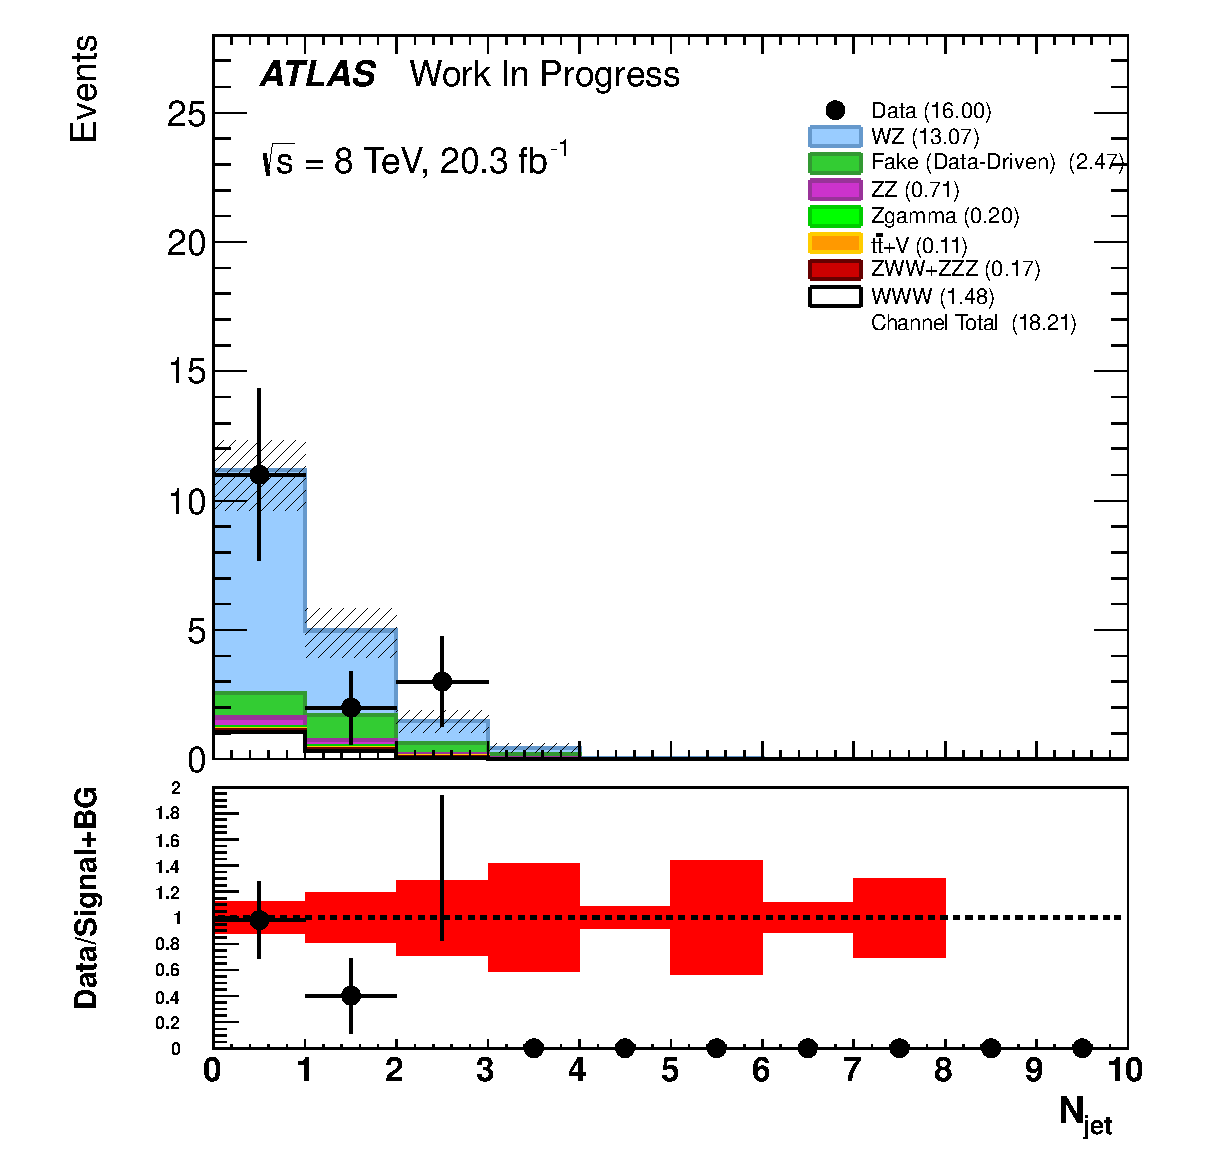
\includegraphics[width=0.3\columnwidth]{figures/appendix_signal_selection/Nov24Update_FakeSys_KFacSys_LinearY_Rebin/output/jobs/MxM/DataFull_Rates_May13_FakeRatesExactly2Loose_MuonMxMBJetGt0_ElBJetGt0SubtractPC_MxM/PreselectionNov23_15_1SFOS_ChargeAbs1_BVeto85_ZVetoLow35High25GeV_METGt45GeV_DeltaPhi2p5_physics/weight_all/eps/NJets_histratio.eps}
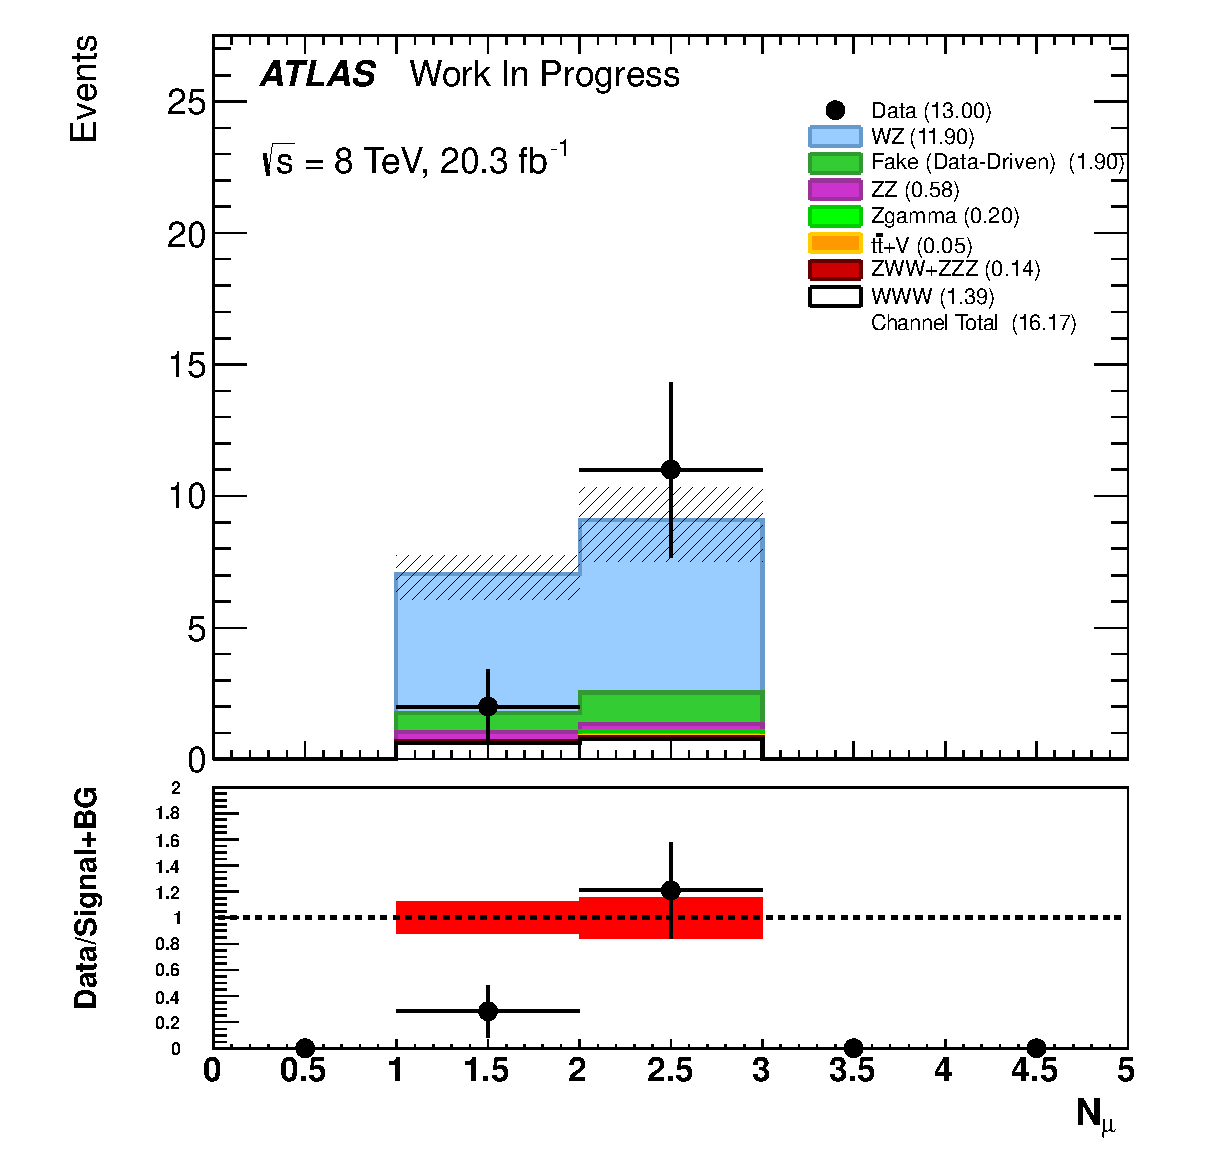
\includegraphics[width=0.3\columnwidth]{figures/appendix_signal_selection/Nov24Update_FakeSys_KFacSys_LinearY_Rebin/output/jobs/MxM/DataFull_Rates_May13_FakeRatesExactly2Loose_MuonMxMBJetGt0_ElBJetGt0SubtractPC_MxM/PreselectionNov23_15_1SFOS_ChargeAbs1_BVeto85_ZVetoLow35High25GeV_METGt45GeV_DeltaPhi2p5_NJetLt2_physics/weight_all/eps/NMuons_histratio.eps}


%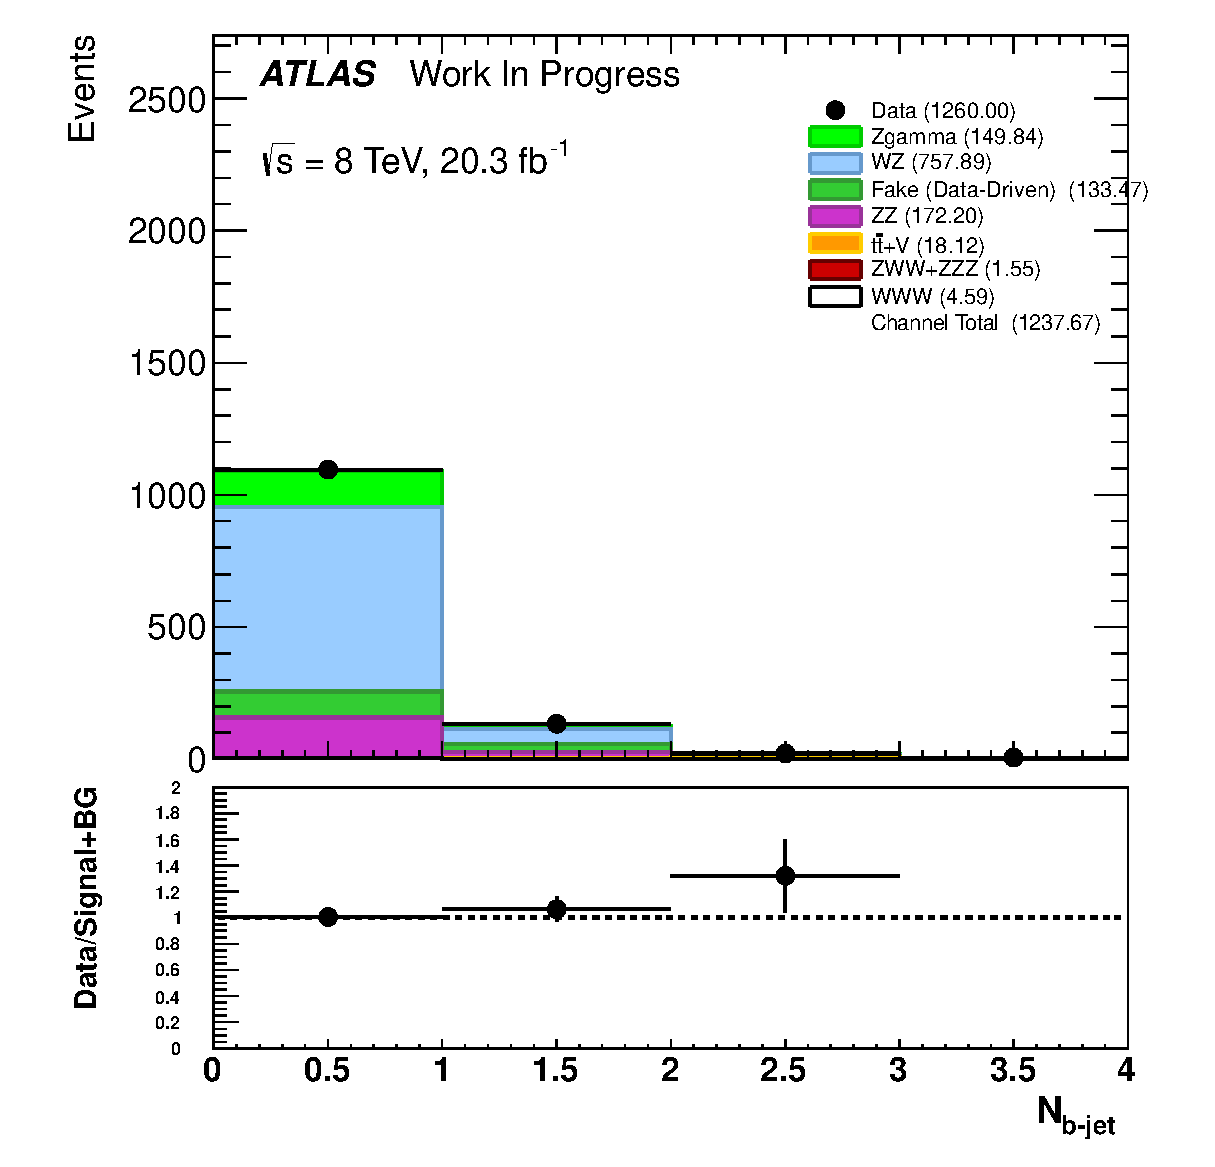
\includegraphics[width=0.3\columnwidth]{figures/appendix_signal_selection/PreselectionMay29_1SFOS_ChargeAbs1_physics/weight_all/eps/NBTaggedJets_histratio.eps}
%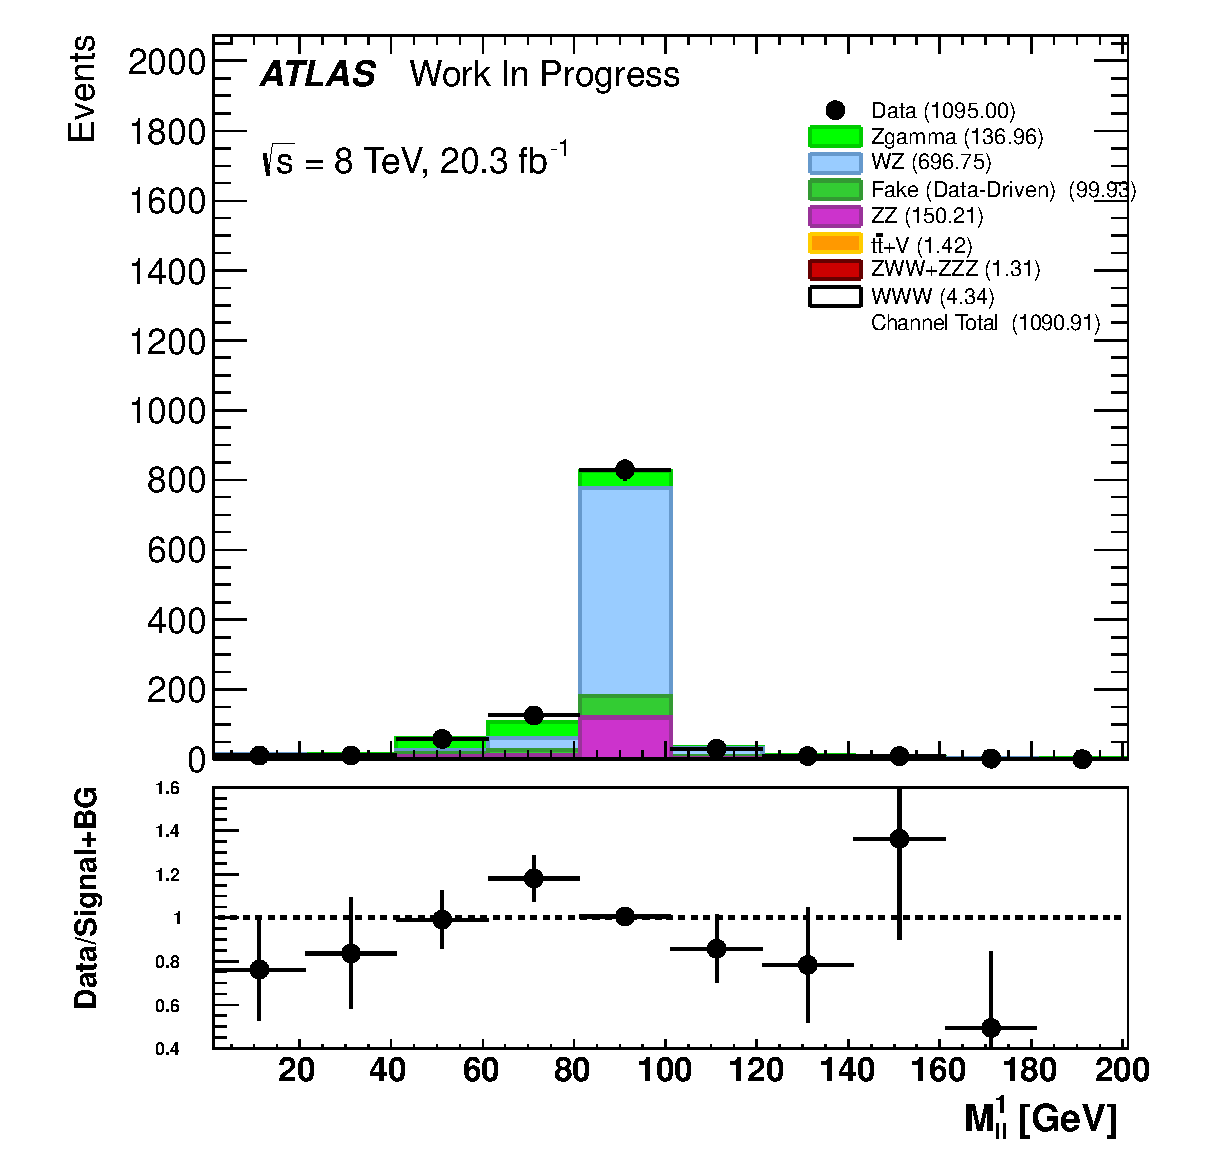
\includegraphics[width=0.3\columnwidth]{figures/appendix_signal_selection/PreselectionMay29_1SFOS_ChargeAbs1_BVeto85_physics/weight_all/eps/InvariantMassSFOS_histratio.eps}
%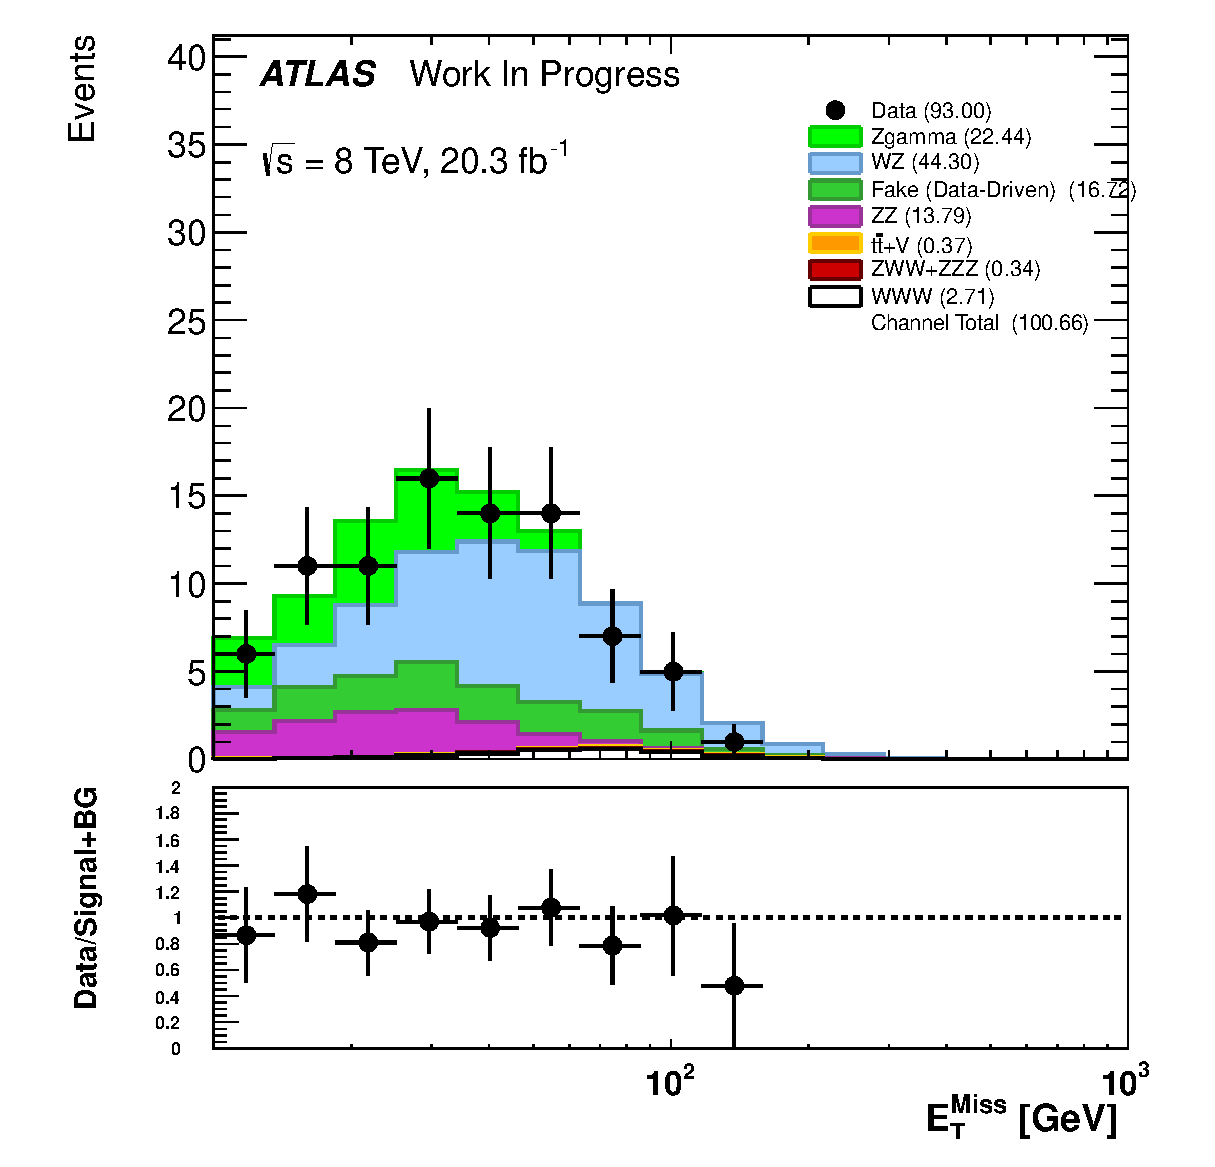
\includegraphics[width=0.3\columnwidth]{figures/appendix_signal_selection/PreselectionMay29_1SFOS_ChargeAbs1_ZVetoLow35High25GeV_physics/weight_all/eps/MET_Et_histratio.eps}
%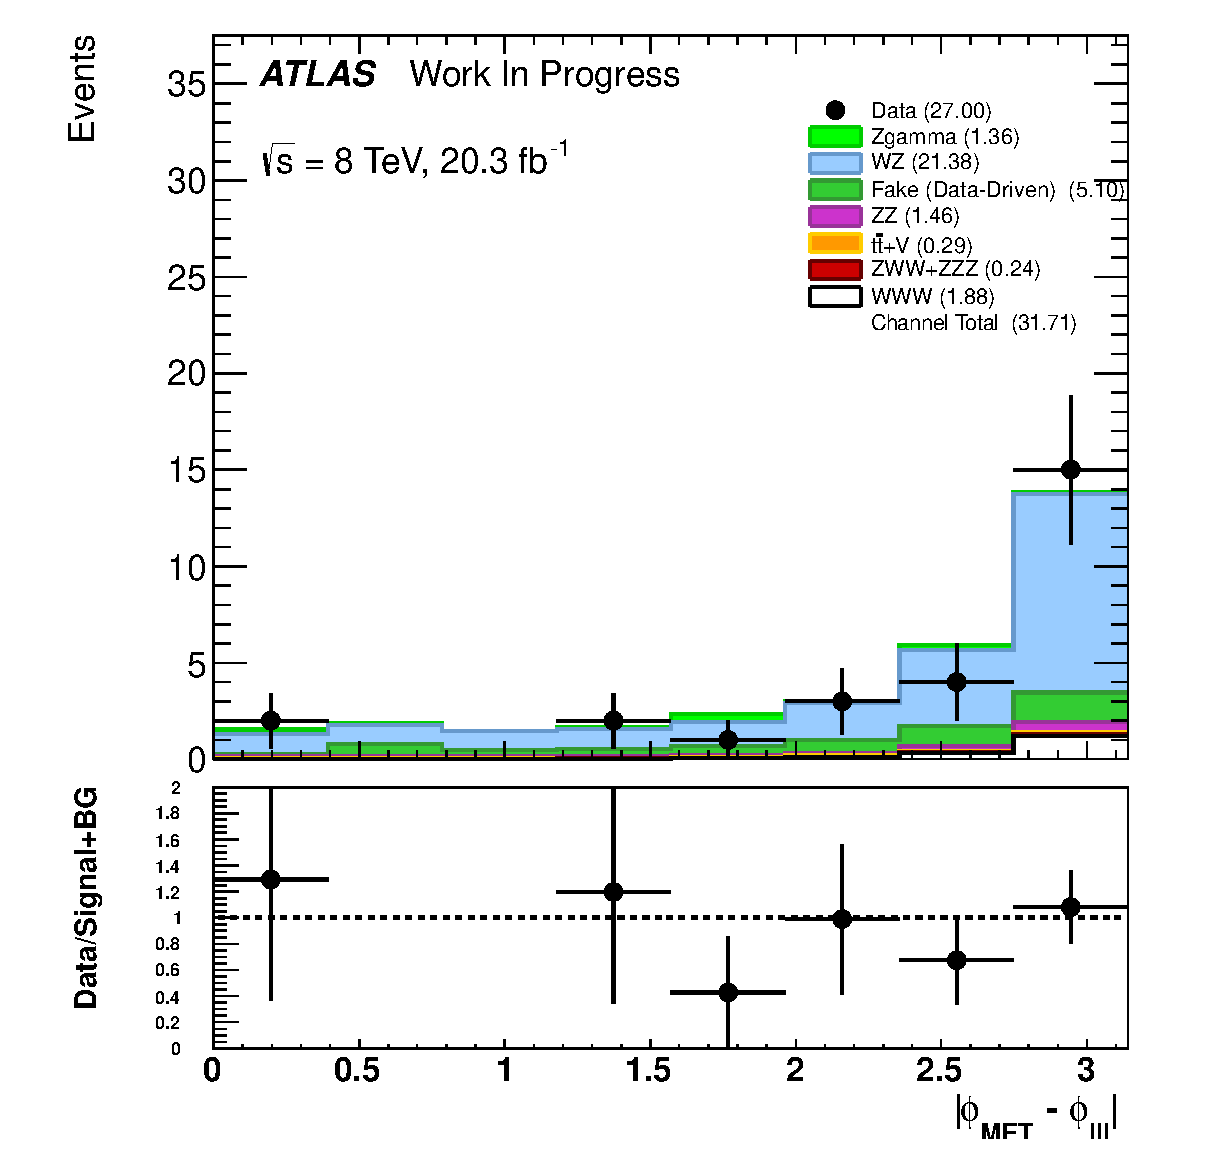
\includegraphics[width=0.3\columnwidth]{figures/appendix_signal_selection/PreselectionJune2_NoSTVF_1SFOS_ChargeAbs1_ZVetoLow35High25GeV_BVeto85_METGt45GeV_physics/weight_all/eps/DeltaPhiMET123_Abs_histratio.eps}
%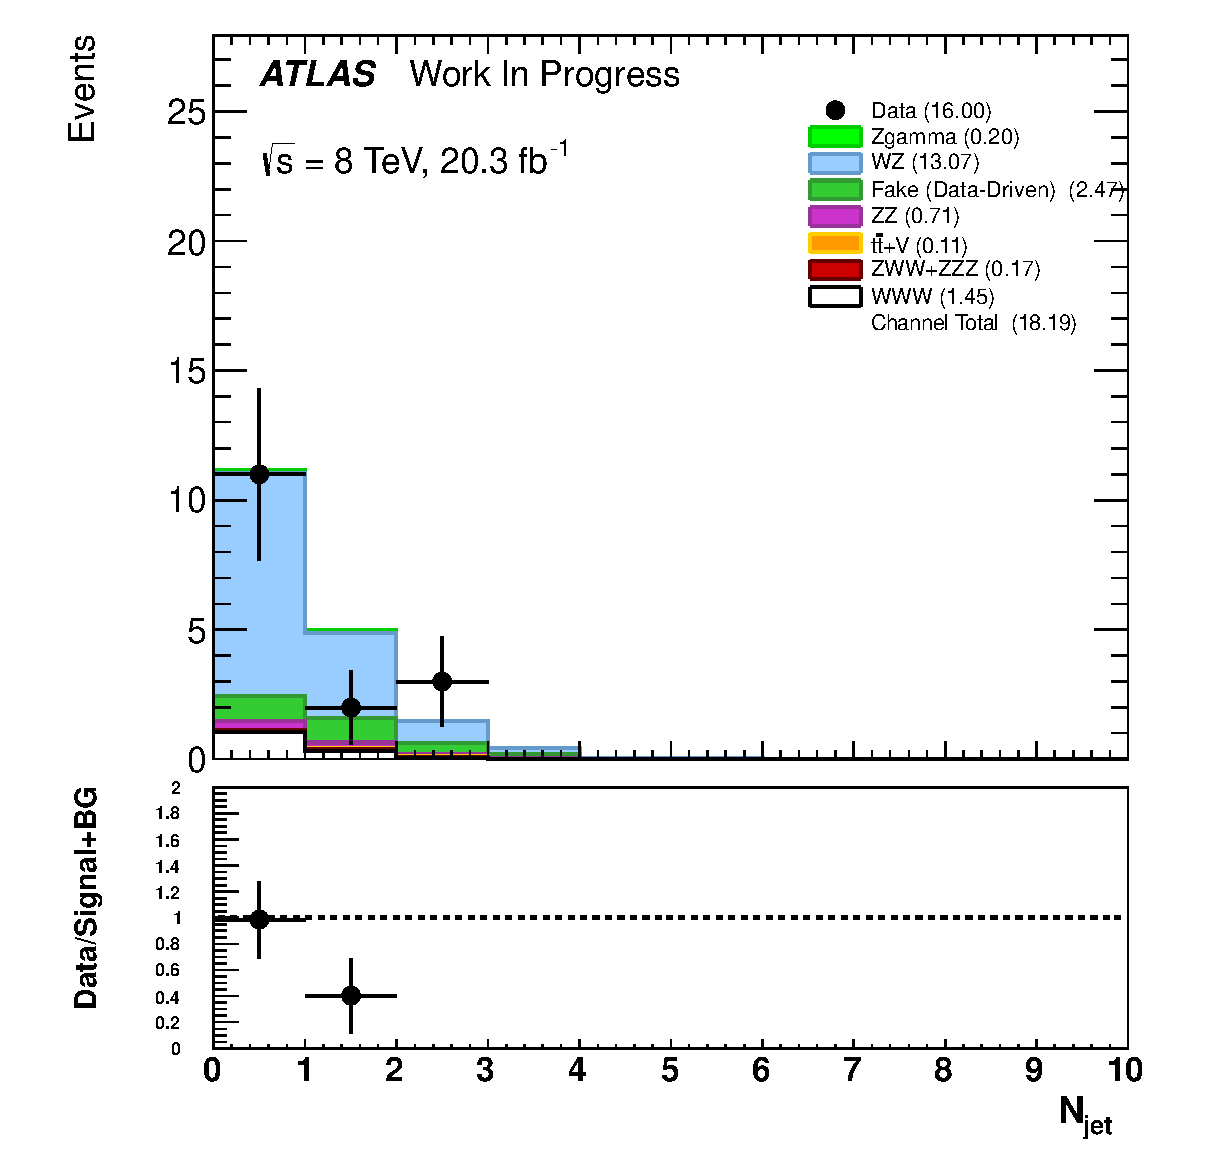
\includegraphics[width=0.3\columnwidth]{figures/appendix_signal_selection/PreselectionJune2_NoSTVF_1SFOS_ChargeAbs1_ZVetoLow35High25GeV_BVeto85_METGt45GeV_DeltaPhi2p5_physics/weight_all/eps/NJets_histratio.eps}
%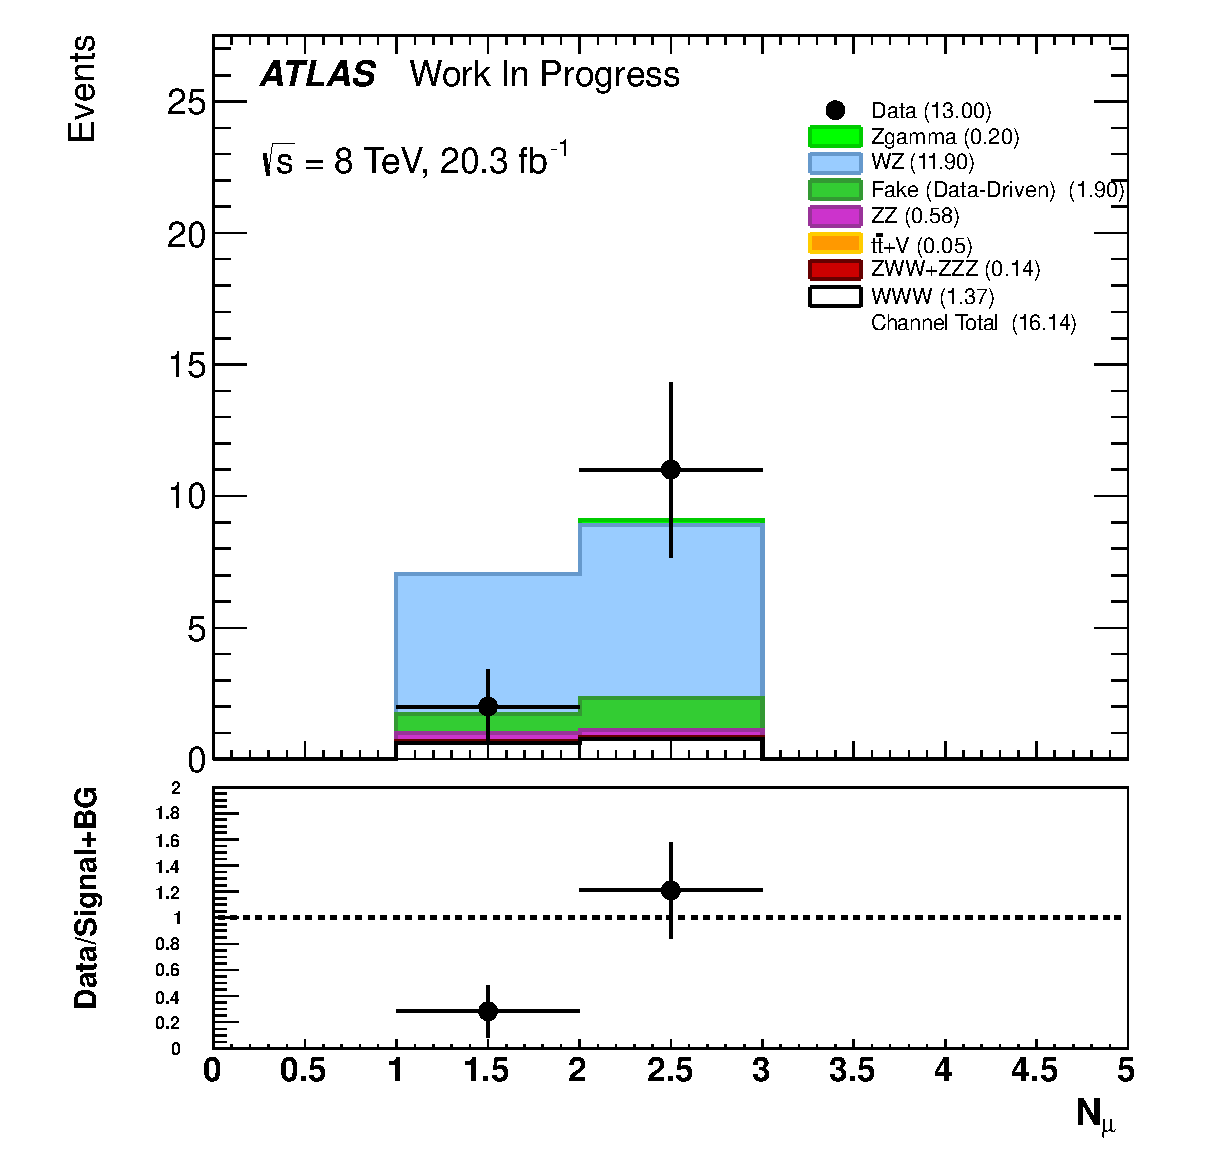
\includegraphics[width=0.3\columnwidth]{figures/appendix_signal_selection/PreselectionJune2_NoSTVF_1SFOS_ChargeAbs1_ZVetoLow35High25GeV_BVeto85_METGt45GeV_DeltaPhi2p5_NJetLt2_physics/weight_all/eps/NMuons_histratio.eps}
\caption{Distributions showing data compared to the signal plus background estimate in the 1 SFOS region at each stage 
of the selection before the cuts are applied to the given distribution. Plots should be read sequentially from left to right
and from top to bottom. 
Referring to Table~\ref{tab:cutflow_weighted_1sfos}, the top left
plot is shown before cut \#3 is applied, top middle is before cut \#4, and
so on until the bottom right which is after all cuts are applied.}
\label{fig:1sfos}
\end{figure}



The 1 SFOS signal region is not as sensitive as the 0 SFOS region, with 
a signal to background ratio of about 9.2\%.
The background is overwhelmingly dominated by $WZ$ contributions. 
Similar to the 0 SFOS region, the predictions and data
at each stage of the 1 SFOS signal region selection are shown in
\tab\ref{tab:cutflow_weighted_1sfos}
and 
\tab\ref{tab:cutflow_weighted_1sfos_bg}. 
The 1 SFOS requirement leaves much of the $WZ$ and $ZZ$ backgrounds,
but the \z-veto and \MET~cuts
are very effective at removing most of this while keeping the signal.


Again, we can also see the signal plus background predictions as 
compared to the data
for the distribution just before each cut is applied in 
the 1 SFOS region by looking at \fig\ref{fig:1sfos}. 
Here, the distributions again appear to be well modeled
at each stage of the selection.  Looking closer
at the \njet~distribution, we can see that there is a deficit
of data in the $\njet=1$ bin which is kept in the seleciton
and results in a slight deficit in the prediction. 
Further, if we look at the \nmu~distibution we see that
this deficit seems to fall exclusively in the $\nmu=1$ bin.
A more detailed investigation of the cutflows
in the individual $\nmu=1$ and $\nmu=2$ bins suggests that 
this is most likely a statisitcal fluctuation.
Overall, the deficit is not very significant, with the Poisson
probability of observing 13 or less events with 16.16 expected
being 26.2\%.


The fake background is only the second largest background in 
this region, making up about 13\% of the total. Still, even with 
the 10\% uncertainty on the normalization of the dominant $WZ$
background, the fake background uncertainty is the largest
uncertainty on the background estimation, approaching 13\%, as
can be seen in \tab\ref{tab:sys_breakdown}.
The \ttV~ and $VVV$ backgrounds are of a similar absolute size as in
the 0 SFOS region, but the larger overall background makes them
even less important. The DPS and $Z\gamma$ uncertainties
contribute a finite amount to the background within the statistical
uncertainties, but remain negligible.

%\begin{table}[ht!]
%\centering
%\begin{tabular}{|c||c|c|c|c|}
\hline
 & $eee$ & $ee\mu$ & $e\mu\mu$ & $\mu\mu\mu$\\ 
\hline\hline
$WZ$ &  $0.0 \pm 0$ &  $5.321 \pm 0.099$ &  $6.58 \pm 0.11$ &  $0.0 \pm 0$\\ 
$ZZ$ &  $0.0 \pm 0$ &  $0.324 \pm 0.012$ &  $0.259 \pm 0.011$ &  $0.0 \pm 0$\\ 
$Z\gamma$ &  $0.0 \pm 0$ &  $0.0 \pm 0$ &  $0.20 \pm 0.13$ &  $0.0 \pm 0$\\ 
$ZWW+ZZZ$ &  $0.0 \pm 0$ &  $0.0660 \pm 0.0077$ &  $0.074 \pm 0.008$ &  $0.0 \pm 0$\\ 
$t\bar{t}+V$ &  $0.0 \pm 0$ &  $0.0207 \pm 0.0031$ &  $0.0296 \pm 0.0036$ &  $0.0 \pm 0$\\ 
Fake (data-driven) &  $0.0 \pm 0$ &  $0.71 \pm 0.18$ &  $1.19 \pm 0.29$ &  $0.0 \pm 0$\\ 
$WWW$ &  $0.0 \pm 0$ &  $0.61 \pm 0.01$ &  $0.760 \pm 0.012$ &  $0.0 \pm 0$\\ 
\hline
Expected Background &  $0.0 \pm 0$ &  $6.44 \pm 0.21$ &  $8.33 \pm 0.34$ &  $0.0 \pm 0$\\ 
Expected Signal + Background &  $0.0 \pm 0$ &  $7.05 \pm 0.21$ &  $9.09 \pm 0.34$ &  $0.0 \pm 0$\\ 
\hline
Observed Data &  $0.0 \pm 0$ &  $2.0 \pm 1.4$ &  $11.0 \pm 3.3$ &  $0.0 \pm 0$\\ 
\hline
\end{tabular}

%\caption{ Expected and observed event yields binned by lepton flavor combination for the optimized 1 SFOS signal region selection defined as follows: event pre-selection + 1 SFOS + b-veto + Z-veto + $\Delta\phi$ + $N_{jet}$ requirements.
%Only statistical uncertainties are shown.
%}
%\label{tab:1sfos}
%\end{table}

\subsubsection{2 SFOS Signal Region}

\begin{table}[ht!]
\small
\centering
%\scriptsize
\begin{tabular}{l||c|c||c|c||c|c}
\hline
 &                 \multicolumn{2}{c||}{Signal}            &  \multicolumn{2}{c||}{Background} &  \multicolumn{2}{c}{Data} \\
   & Yield & Eff. & Yield & Eff. & Yield & Eff.\\
   \hline\hline
   %1. Pre-selection &  $9.78$ & --- &  $2388.48$ & --- & $2472$ &  --- \\ 
   %\hline
   1. 2 SFOS &  $2.66$ &  --- &  $1132.53$ &  --- & $1182$ & ---\\ 
   \hline
   2. $N_{\mathrm{b-jet}}=0$ &  $2.50$ &  $0.94$ &  $1012.07$ &  $0.89$ & $1033$ &  $0.87$\\ 
   \hline
   3. $| m_{\mathrm{SFOS}} - m_Z | >  20$ GeV &  $1.46$ &  $0.58$ &  $108.88$ &  $0.11$ & $108$ &  $0.10$\\ 
   \hline
   4. $E_{T}^{Miss} > 55$ GeV &  $0.83$ &  $0.57$ &  $18.99$ &  $0.17$ & $18$ &  $0.17$\\ 
   \hline
   5. $|\Delta\phi(3l,E_{T}^{Miss})| > 2.5$ &  $0.65$ &  $0.78$ &  $11.64$ &  $0.61$ & $8$ &  $0.44$\\ 
   \hline
   6. $N_{\mathrm{Jet}} \leq 1$ &  $0.61$ &  $0.94$ &  $10.25$ &  $0.88$ & $6$ &  $0.75$\\ 
   \hline
   \end{tabular}



\caption{Cut-flows showing the event yields and efficiencies for each cut in the 2 SFOS signal region
starting from event pre-selection separately for the total signal and total background predictions, along with the observed data.
Event yields for MC backgrounds and signal include all weights and are normalized to an integrated luminosity of $20.3~\mathrm{fb}^{-1}$.  
The fake lepton background only includes the matrix method weights.  The data is unweighted.
Efficiencies show the ratio of the yield with respect
to the previous cut.  The efficiency is first calculated at the first cut after event pre-selection.  }
\label{tab:cutflow_weighted_2sfos}
\end{table}

\begin{table}[ht!]
\small
\centering
%\scriptsize
\begin{tabular}{l||c|c||c|c||c|c}
\hline
 &       \multicolumn{6}{c}{Background} \\
 & \multicolumn{2}{c||}{$WZ$} & \multicolumn{2}{c||}{$ZZ$} & \multicolumn{2}{c}{$t\bar{t}+V$}  \\ 
 & Yield & Eff. & Yield & Eff. & Yield & Eff.  \\
\hline\hline
Pre-selection &  $1566.91$ & --- &  $323.60$ & --- &  $36.93$ & --- \\ 
\hline
2 SFOS &  $807.27$ &  $0.52$ &  $151.28$ &  $0.47$ &  $15.35$ &  $0.42$  \\ 
\hline
$N_{\mathrm{b-jet}}=0$ &  $743.12$ &  $0.92$ &  $136.16$ &  $0.90$ &  $1.19$ &  $0.08$ \\ 
\hline
$| m_{\mathrm{SFOS}} - m_Z | >  20$ GeV &  $44.95$ &  $0.06$ &  $21.13$ &  $0.16$ &  $0.22$ &  $0.18$\\ 
\hline
$E_{T}^{Miss} > 55$ GeV &  $15.86$ &  $0.35$ &  $0.97$ &  $0.05$ &  $0.14$ &  $0.65$ \\ 
\hline
$|\Delta\phi(3l,E_{T}^{Miss})| > 2.5$ &  $10.09$ &  $0.64$ &  $0.55$ &  $0.57$ &  $0.07$ &  $0.49$ \\ 
\hline
$N_{\mathrm{Jet}} \leq 1$ &  $9.07$ &  $0.90$ &  $0.48$ &  $0.86$ &  $0.02$ &  $0.35$ \\ 
\hline
\end{tabular}


\begin{tabular}{l||c|c||c|c||c|c}
\hline
 &       \multicolumn{6}{c}{Background} \\
 & \multicolumn{2}{c||}{$ZZZ+ZWW$} & \multicolumn{2}{c||}{$Z\gamma$} & \multicolumn{2}{c}{Fake} \\ 
 & Yield & Eff. & Yield & Eff. & Yield & Eff. \\
\hline\hline
Pre-selection & $3.12$ & --- &  $219.80$ & --- &  $238.12$ & ---  \\ 
\hline
1. 2 SFOS &  $1.30$ &  $0.41$ &  $69.99$ &  $0.32$ &  $87.34$ &  $0.37$ \\ 
\hline
2. $N_{\mathrm{b-jet}}=0$ &  $1.10$ &  $0.85$ &  $64.70$ &  $0.92$ &  $65.80$ &  $0.75$ \\ 
\hline
3. $| m_{\mathrm{SFOS}} - m_Z | >  20$ GeV &  $0.19$ &  $0.17$ &  $29.52$ &  $0.46$ &  $12.87$ &  $0.20$ \\ 
\hline
4. $E_{T}^{Miss} > 55$ GeV &  $0.12$ &  $0.63$ &  $0.43$ &  $0.01$ &  $1.47$ &  $0.11$ \\ 
\hline
5. $|\Delta\phi(3l,E_{T}^{Miss})| > 2.5$ &  $0.10$ &  $0.82$ &  $0.11$ &  $0.25$ &  $0.72$ &  $0.49$ \\ 
\hline
6. $N_{\mathrm{Jet}} \leq 1$ &  $0.08$ &  $0.82$ &  $0.11$ &  $1.00$ &  $0.49$ &  $0.69$ \\ 
\hline
\end{tabular}


\caption{Cut-flows showing the event yields and efficiencies for each cut in the 2 SFOS signal region
starting from event pre-selection and binned by background category. 
Event yields for MC backgrounds and signal include all weights and are normalized to an integrated luminosity of $20.3~\mathrm{fb}^{-1}$.  
The fake lepton background only includes the matrix method weights.  The data is unweighted.
Efficiencies show the ratio of the yield with respect
to the previous cut.  The efficiency is first calculated at the first cut after event pre-selection.  }
\label{tab:cutflow_weighted_2sfos_bg}
\end{table}


%2 SFOS consolidated
\begin{figure}[ht!]
\centering
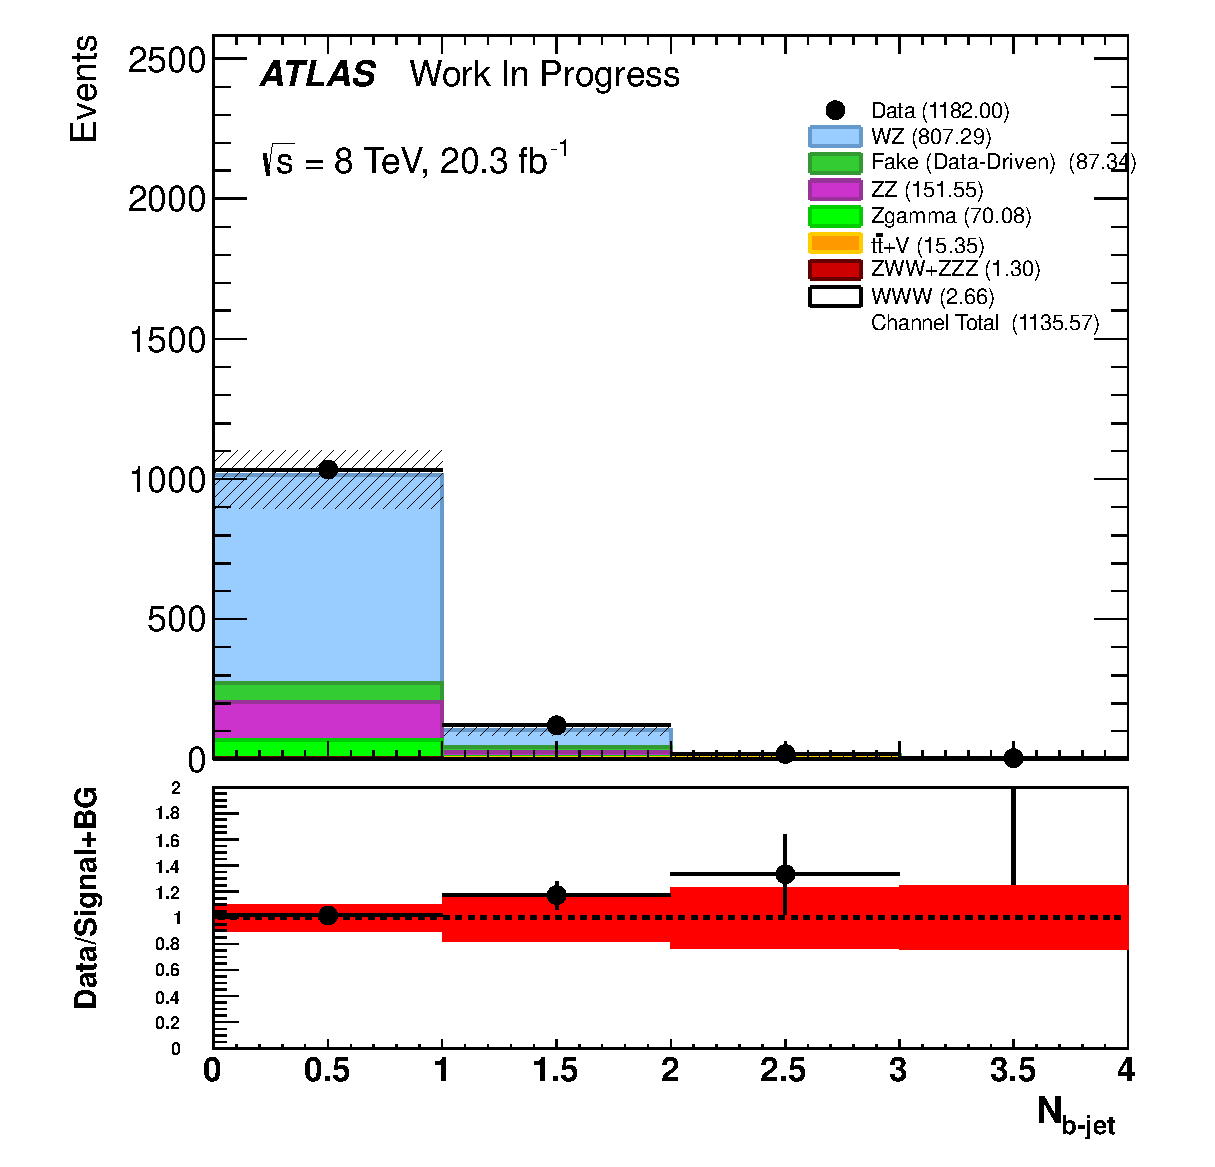
\includegraphics[width=0.3\columnwidth]{figures/appendix_signal_selection/Nov24Update_FakeSys_KFacSys_LinearY_Rebin/output/jobs/MxM/DataFull_Rates_May13_FakeRatesExactly2Loose_MuonMxMBJetGt0_ElBJetGt0SubtractPC_MxM/PreselectionNov23_15_2SFOS_ChargeAbs1_physics/weight_all/eps/NBTaggedJets_histratio.eps}
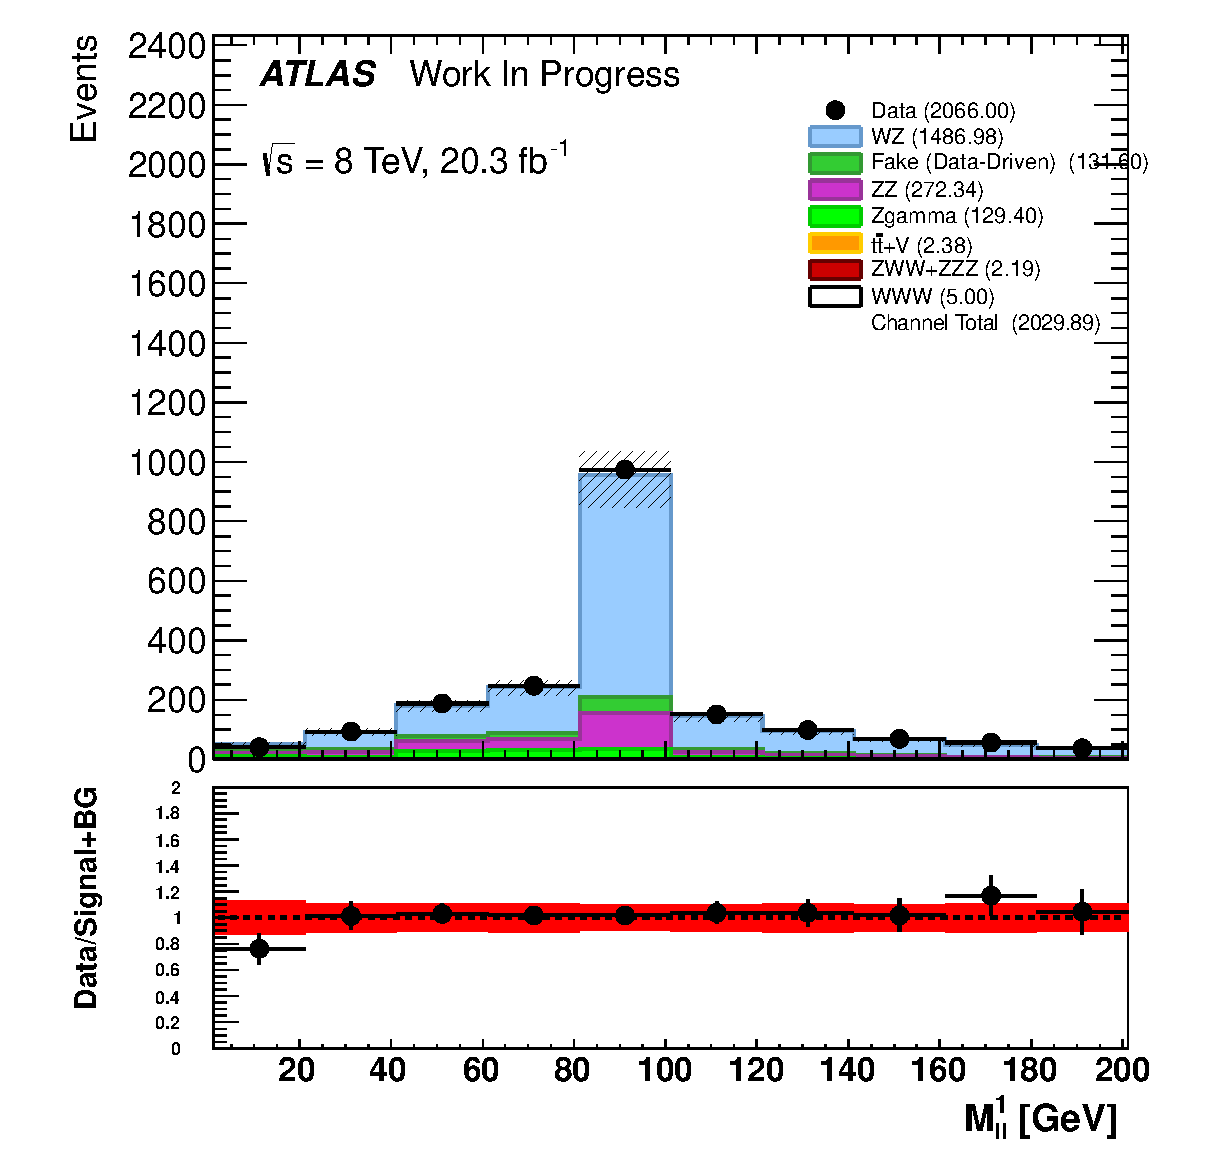
\includegraphics[width=0.3\columnwidth]{figures/appendix_signal_selection/Nov24Update_FakeSys_KFacSys_LinearY_Rebin/output/jobs/MxM/DataFull_Rates_May13_FakeRatesExactly2Loose_MuonMxMBJetGt0_ElBJetGt0SubtractPC_MxM/PreselectionNov23_15_2SFOS_ChargeAbs1_BVeto85_physics/weight_all/eps/InvariantMassSFOS_histratio.eps}
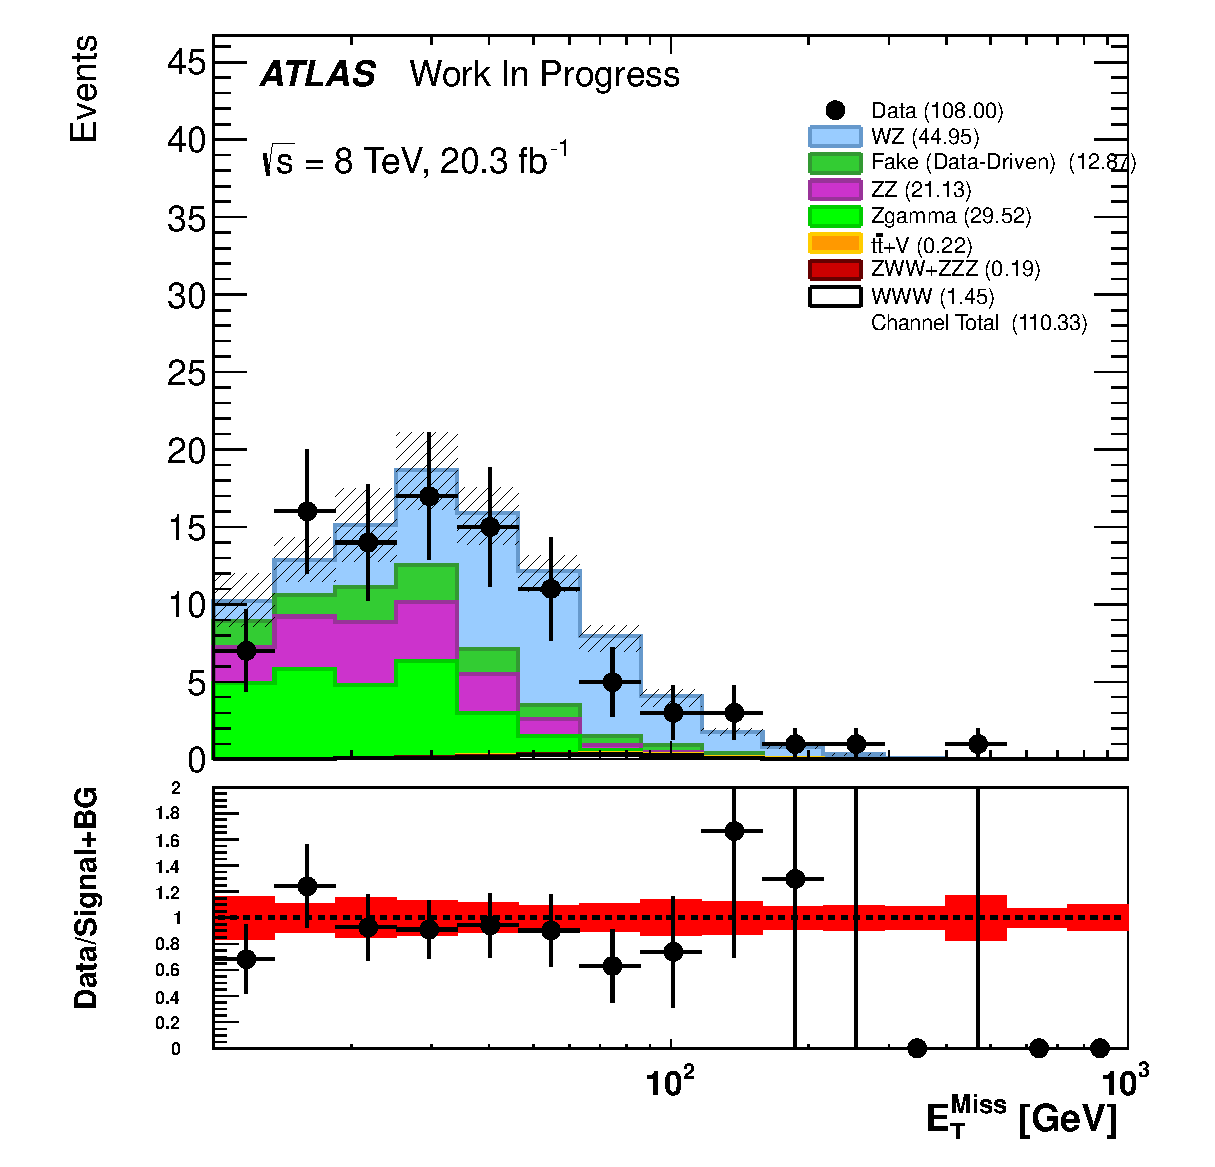
\includegraphics[width=0.3\columnwidth]{figures/appendix_signal_selection/Nov24Update_FakeSys_KFacSys_LinearY_Rebin/output/jobs/MxM/DataFull_Rates_May13_FakeRatesExactly2Loose_MuonMxMBJetGt0_ElBJetGt0SubtractPC_MxM/PreselectionNov23_15_2SFOS_ChargeAbs1_BVeto85_ZVeto20GeV_physics/weight_all/eps/MET_Et_histratio.eps}
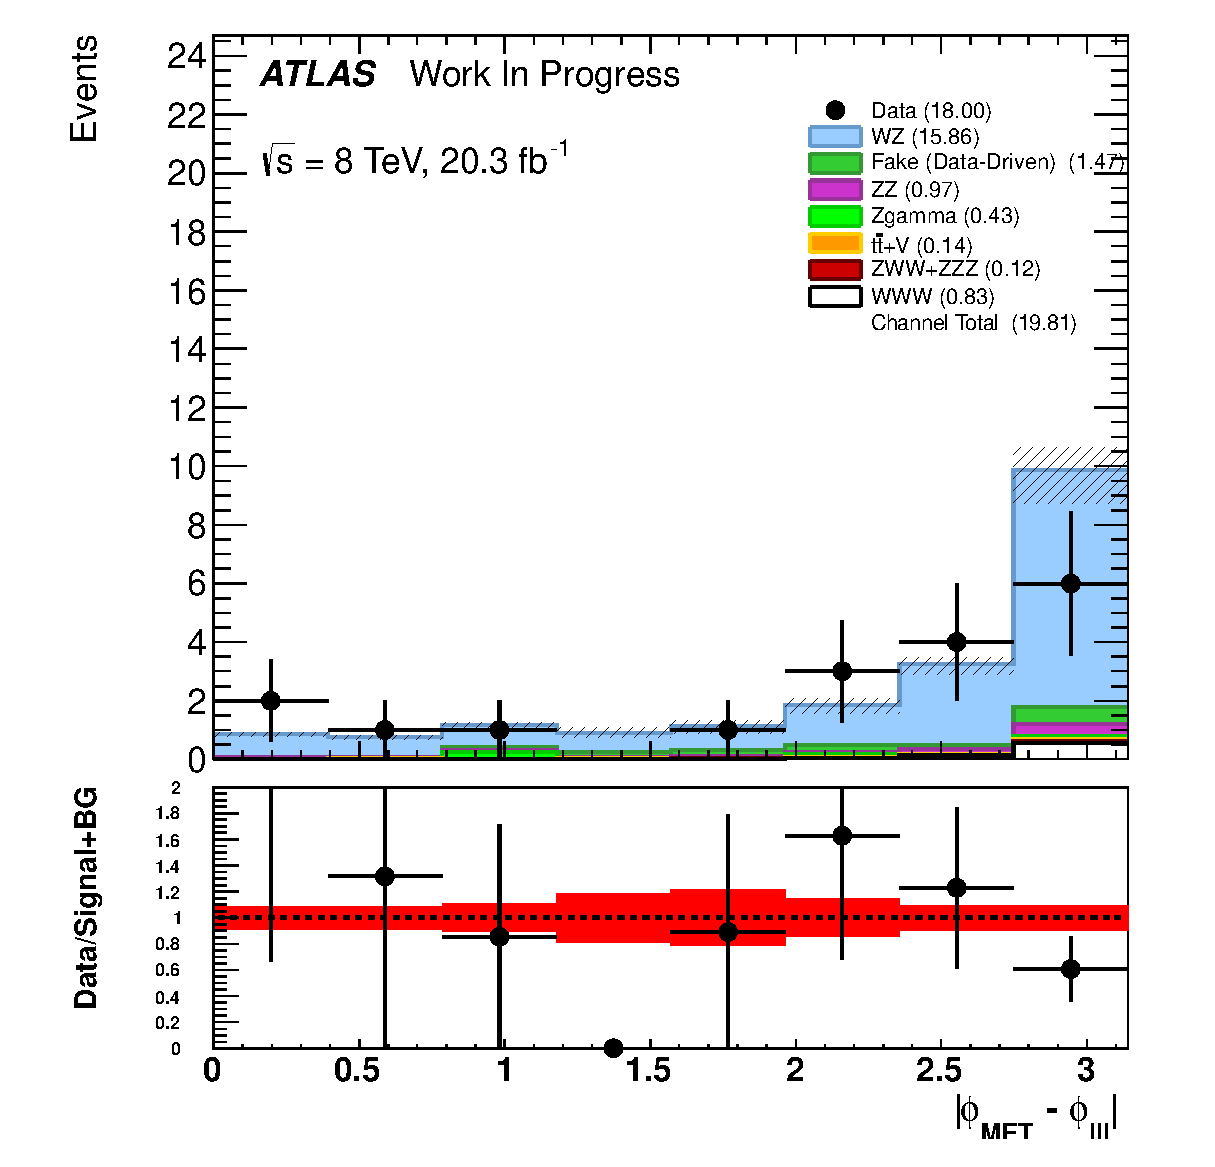
\includegraphics[width=0.3\columnwidth]{figures/appendix_signal_selection/Nov24Update_FakeSys_KFacSys_LinearY_Rebin/output/jobs/MxM/DataFull_Rates_May13_FakeRatesExactly2Loose_MuonMxMBJetGt0_ElBJetGt0SubtractPC_MxM/PreselectionNov23_15_2SFOS_ChargeAbs1_BVeto85_ZVeto20GeV_METGt55GeV_physics/weight_all/eps/DeltaPhiMET123_Abs_histratio.eps}
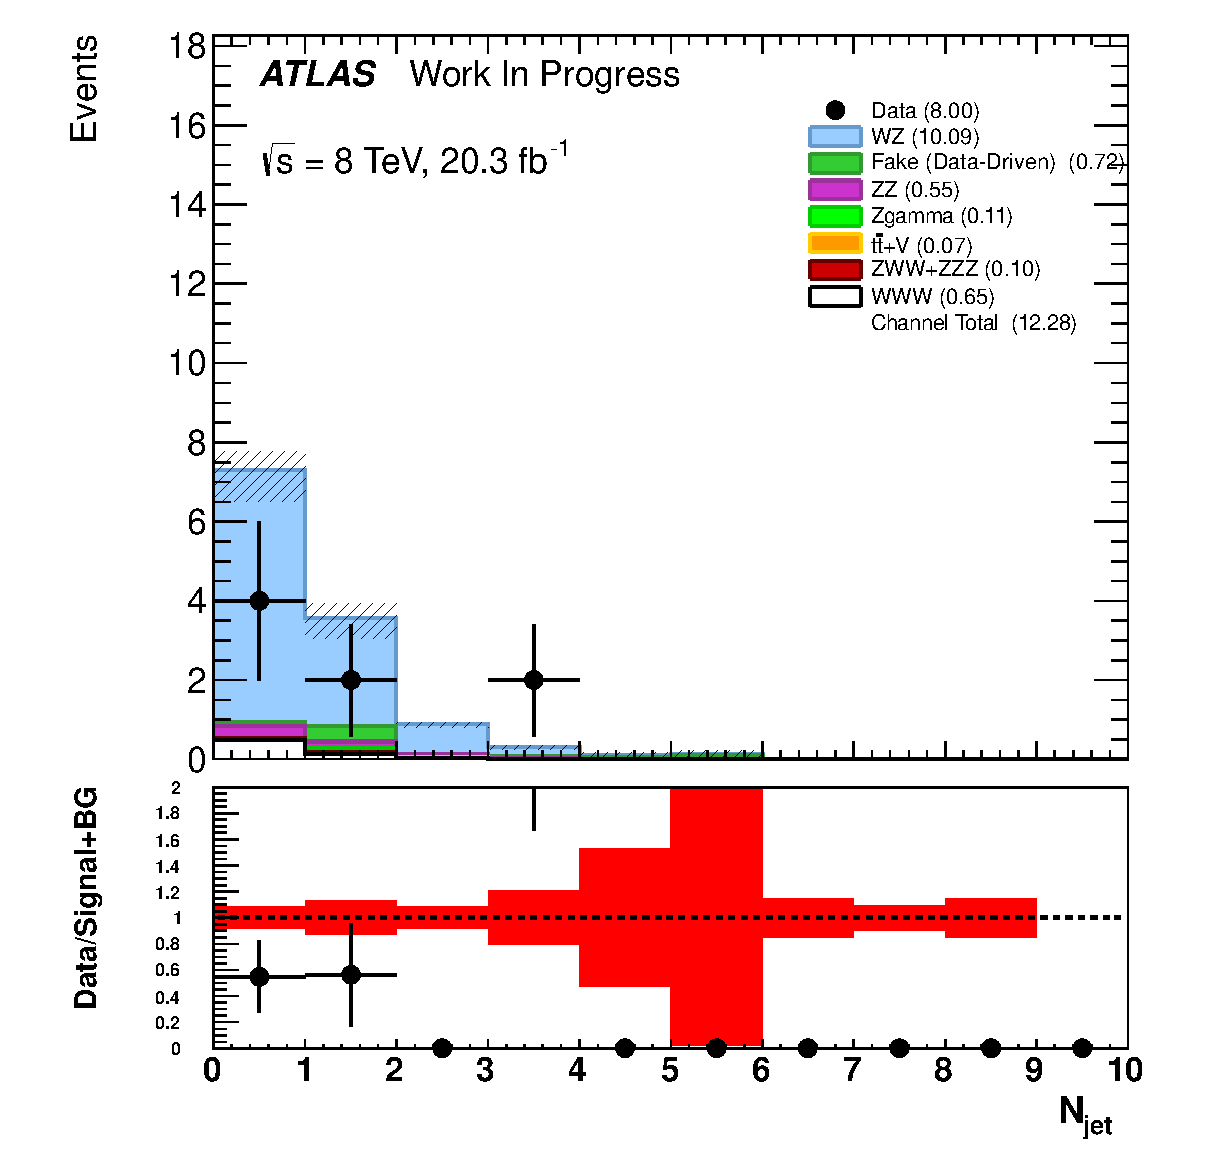
\includegraphics[width=0.3\columnwidth]{figures/appendix_signal_selection/Nov24Update_FakeSys_KFacSys_LinearY_Rebin/output/jobs/MxM/DataFull_Rates_May13_FakeRatesExactly2Loose_MuonMxMBJetGt0_ElBJetGt0SubtractPC_MxM/PreselectionNov23_15_2SFOS_ChargeAbs1_BVeto85_ZVeto20GeV_METGt55GeV_DeltaPhi2p5_physics/weight_all/eps/NJets_histratio.eps}
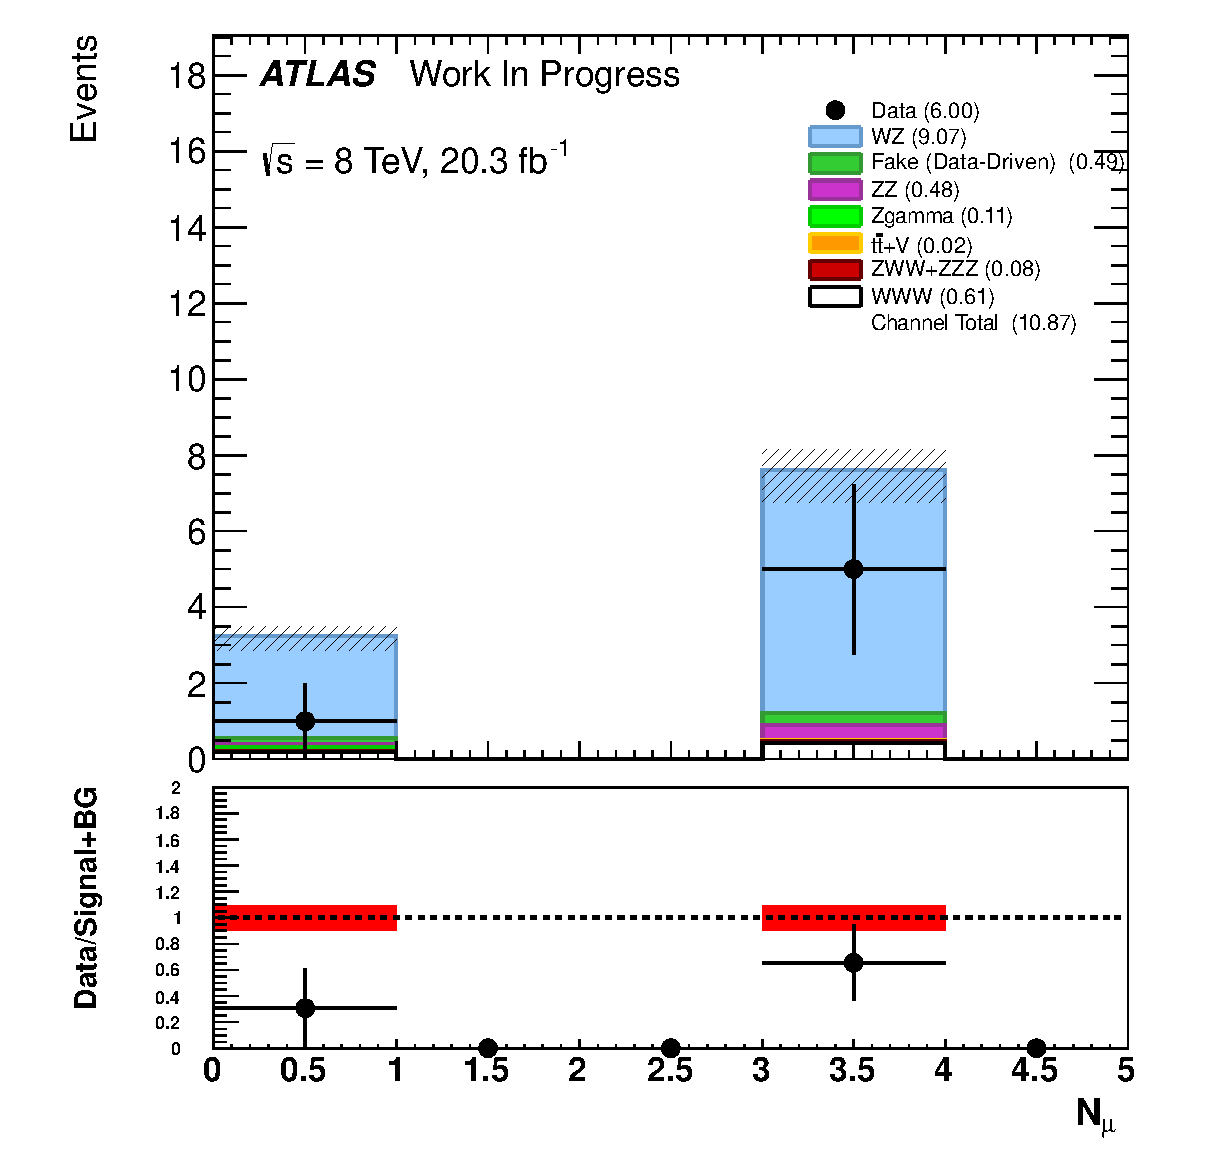
\includegraphics[width=0.3\columnwidth]{figures/appendix_signal_selection/Nov24Update_FakeSys_KFacSys_LinearY_Rebin/output/jobs/MxM/DataFull_Rates_May13_FakeRatesExactly2Loose_MuonMxMBJetGt0_ElBJetGt0SubtractPC_MxM/PreselectionNov23_15_2SFOS_ChargeAbs1_BVeto85_ZVeto20GeV_METGt55GeV_DeltaPhi2p5_NJetLt2_physics/weight_all/eps/NMuons_histratio.eps}



%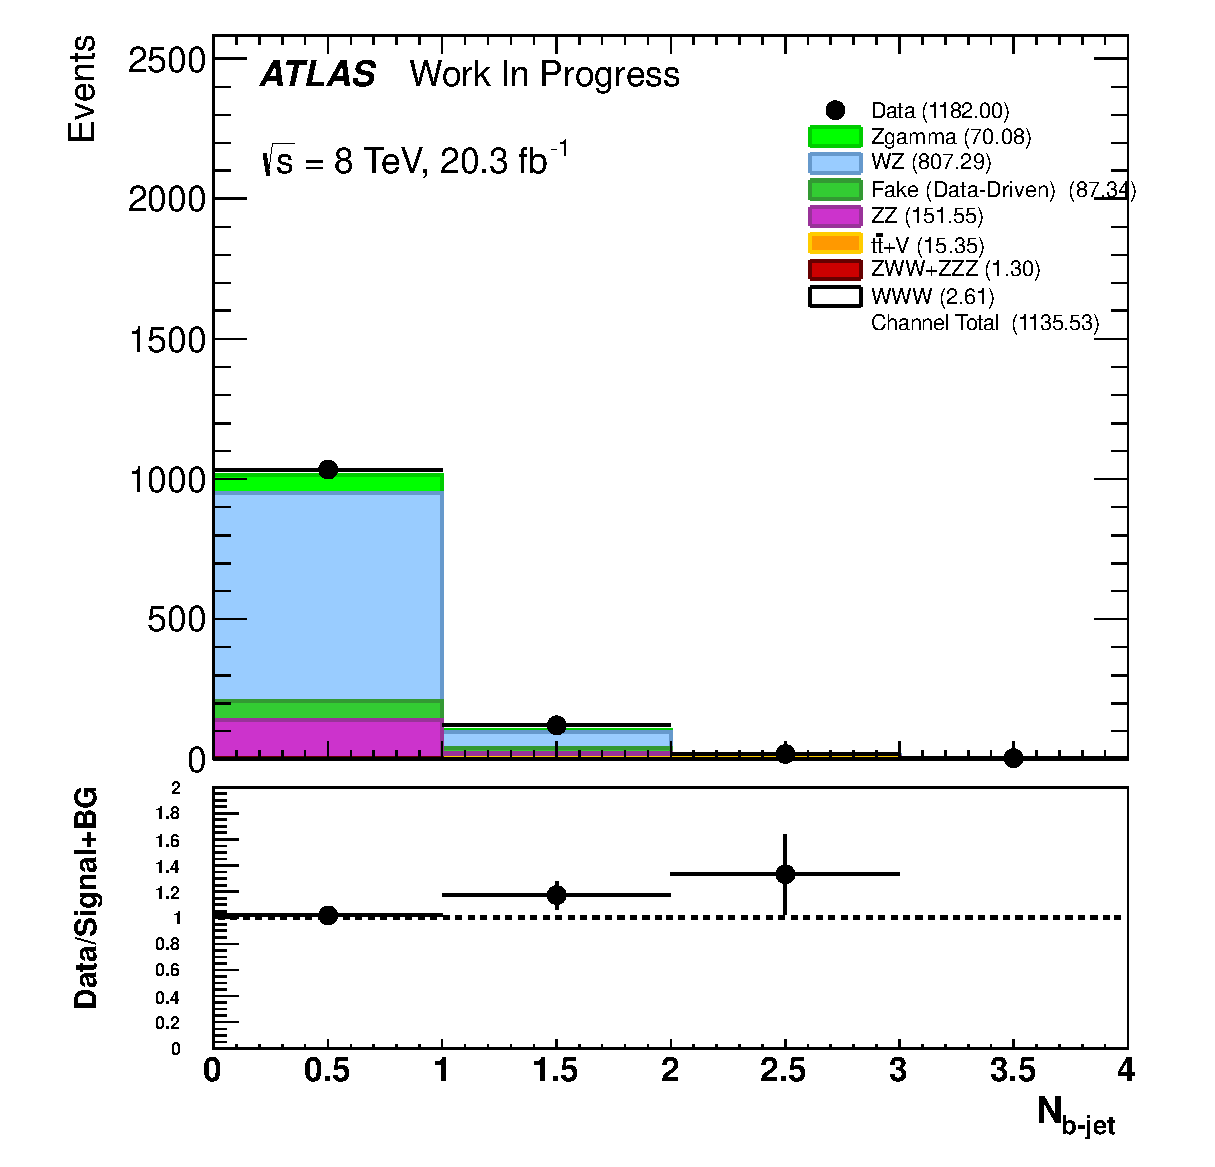
\includegraphics[width=0.3\columnwidth]{figures/appendix_signal_selection/PreselectionMay29_2SFOS_ChargeAbs1_physics/weight_all/eps/NBTaggedJets_histratio.eps}
%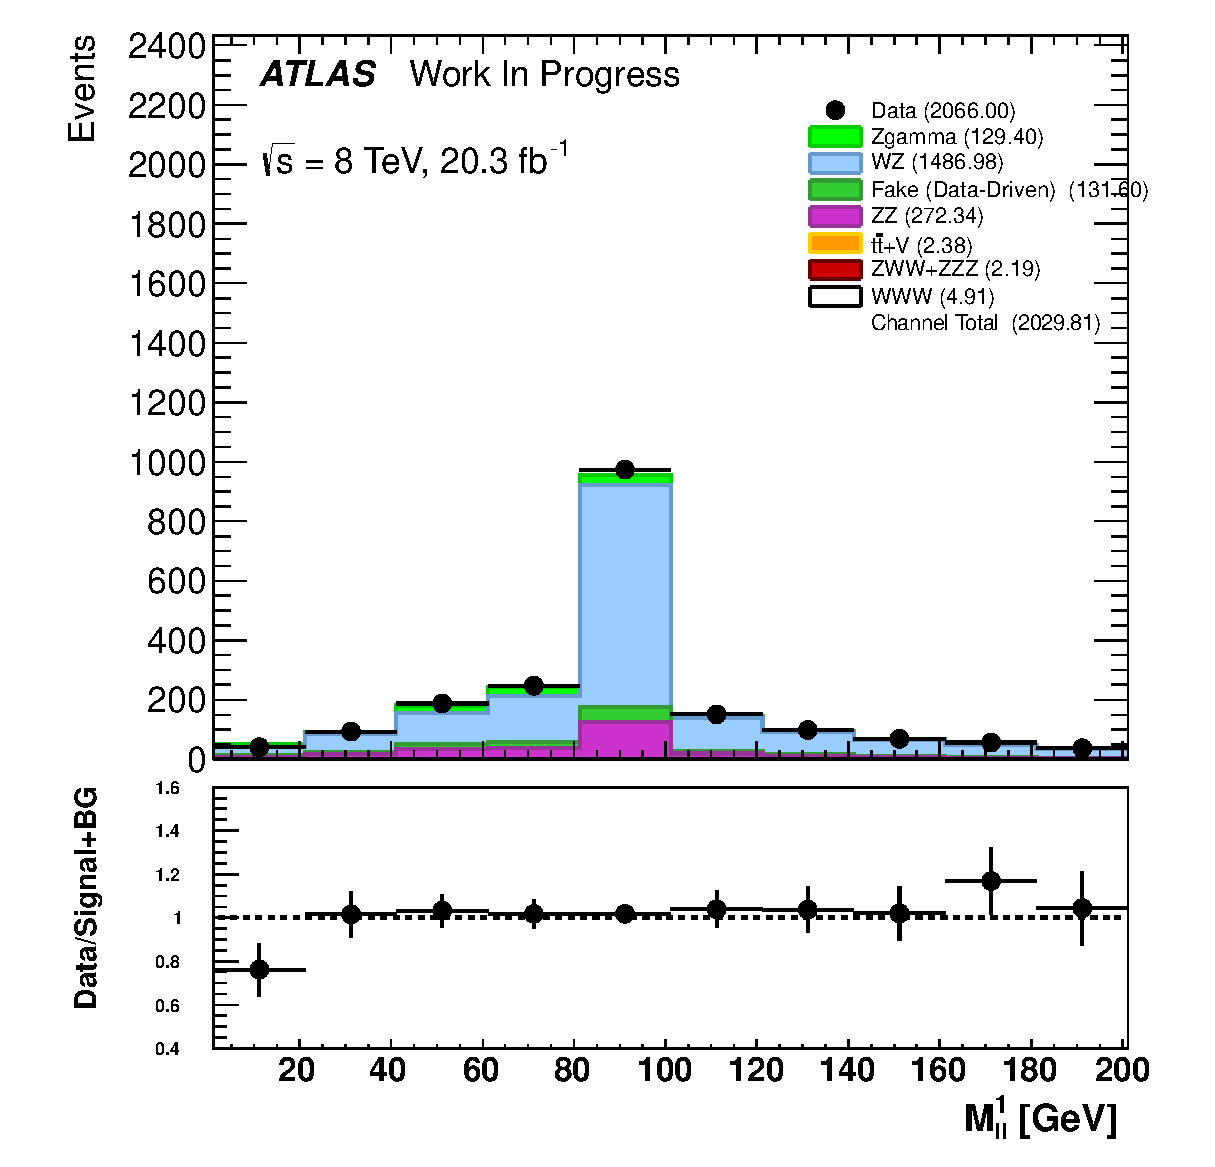
\includegraphics[width=0.3\columnwidth]{figures/appendix_signal_selection/PreselectionMay29_2SFOS_ChargeAbs1_BVeto85_physics/weight_all/eps/InvariantMassSFOS_histratio.eps}
%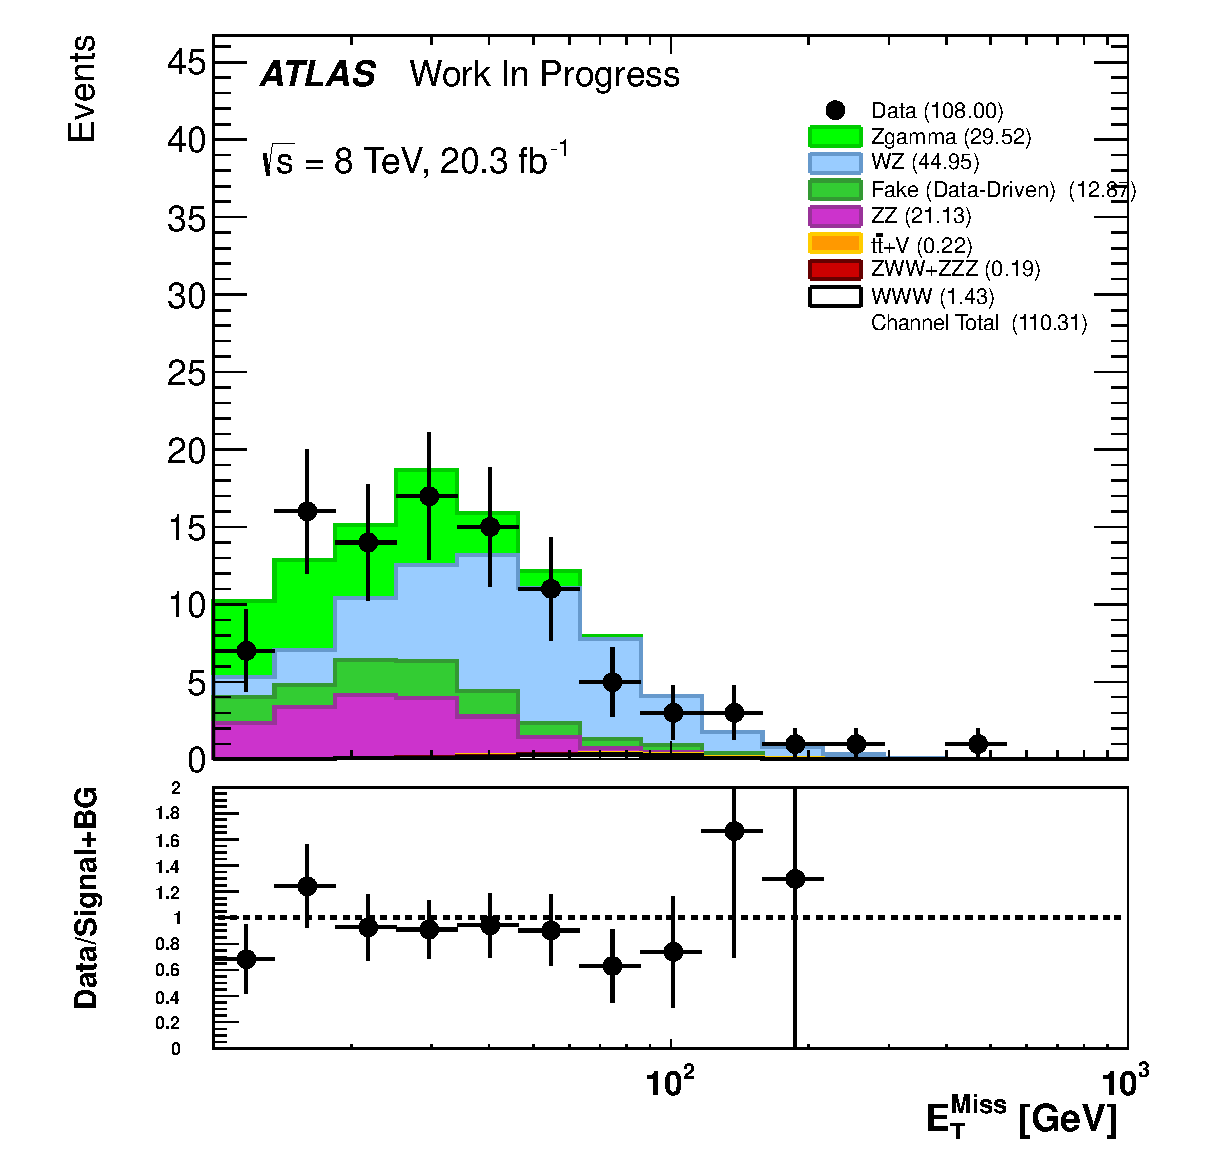
\includegraphics[width=0.3\columnwidth]{figures/appendix_signal_selection/PreselectionMay29_2SFOS_ChargeAbs1_BVeto85_ZVeto20GeV_physics/weight_all/eps/MET_Et_histratio.eps}
%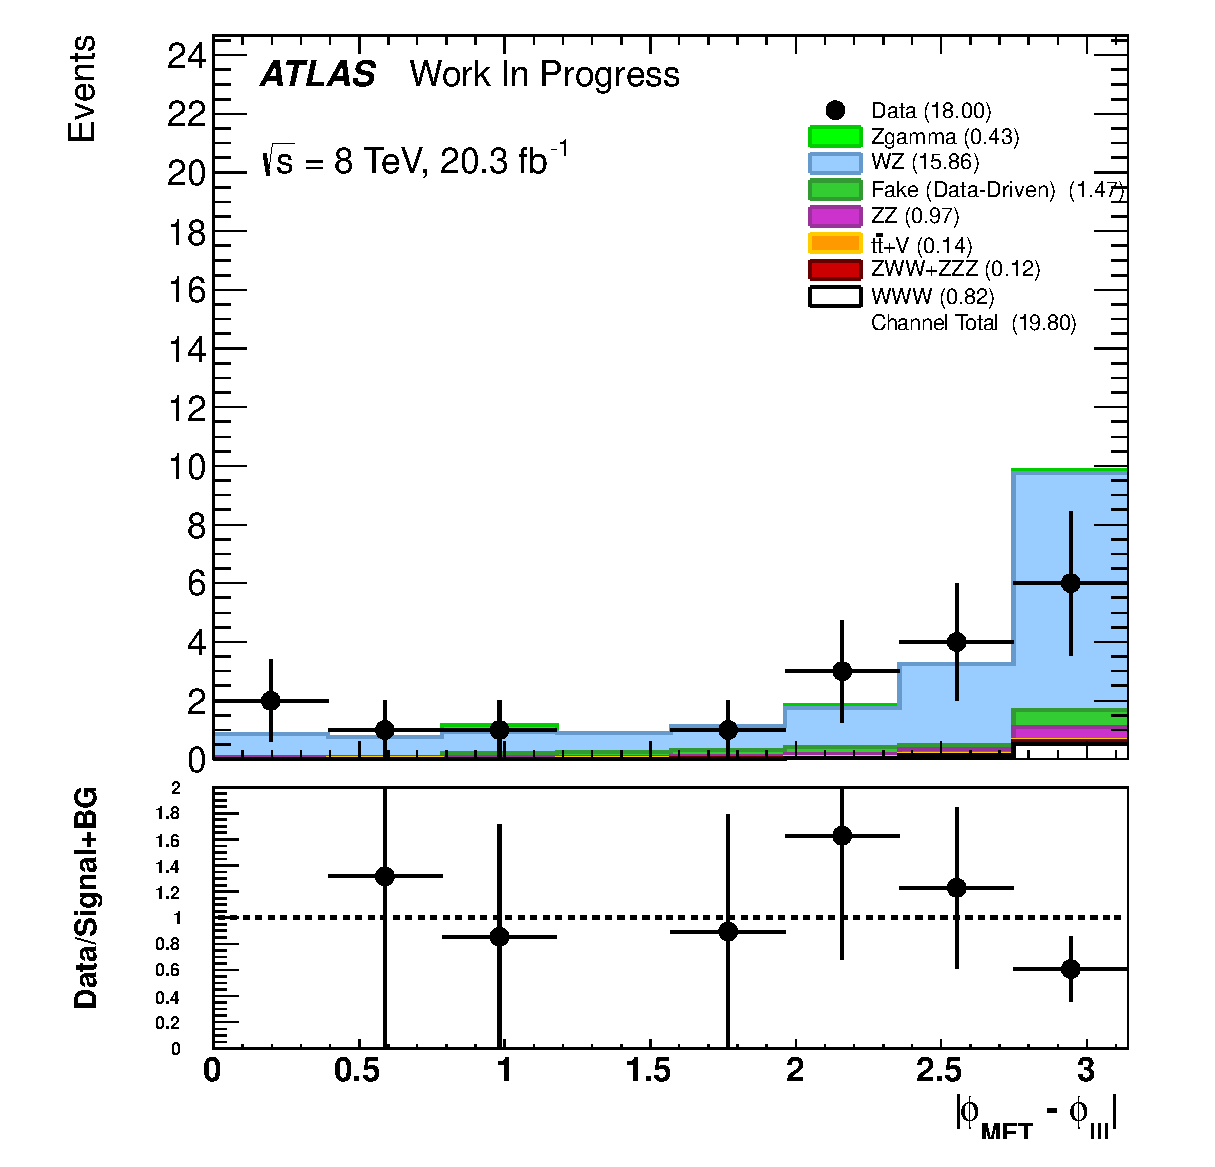
\includegraphics[width=0.3\columnwidth]{figures/appendix_signal_selection/PreselectionJune2_NoSTVF_2SFOS_ChargeAbs1_BVeto85_ZVeto20GeV_METGt55GeV_physics/weight_all/eps/DeltaPhiMET123_Abs_histratio.eps}
%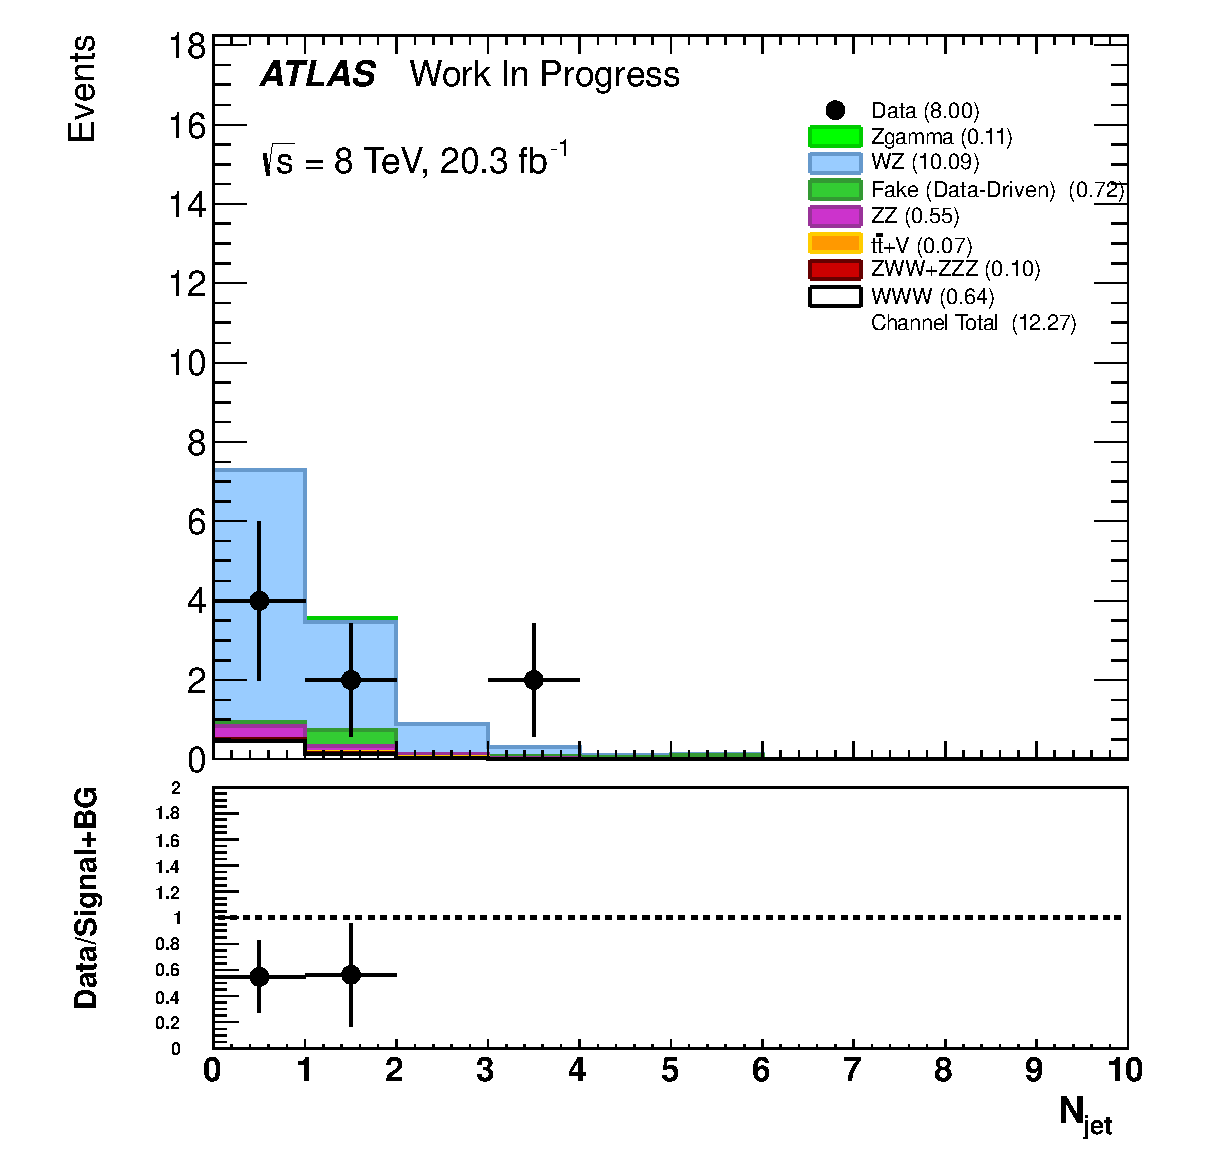
\includegraphics[width=0.3\columnwidth]{figures/appendix_signal_selection/PreselectionJune2_NoSTVF_2SFOS_ChargeAbs1_BVeto85_ZVeto20GeV_METGt55GeV_DeltaPhi2p5_physics/weight_all/eps/NJets_histratio.eps}
%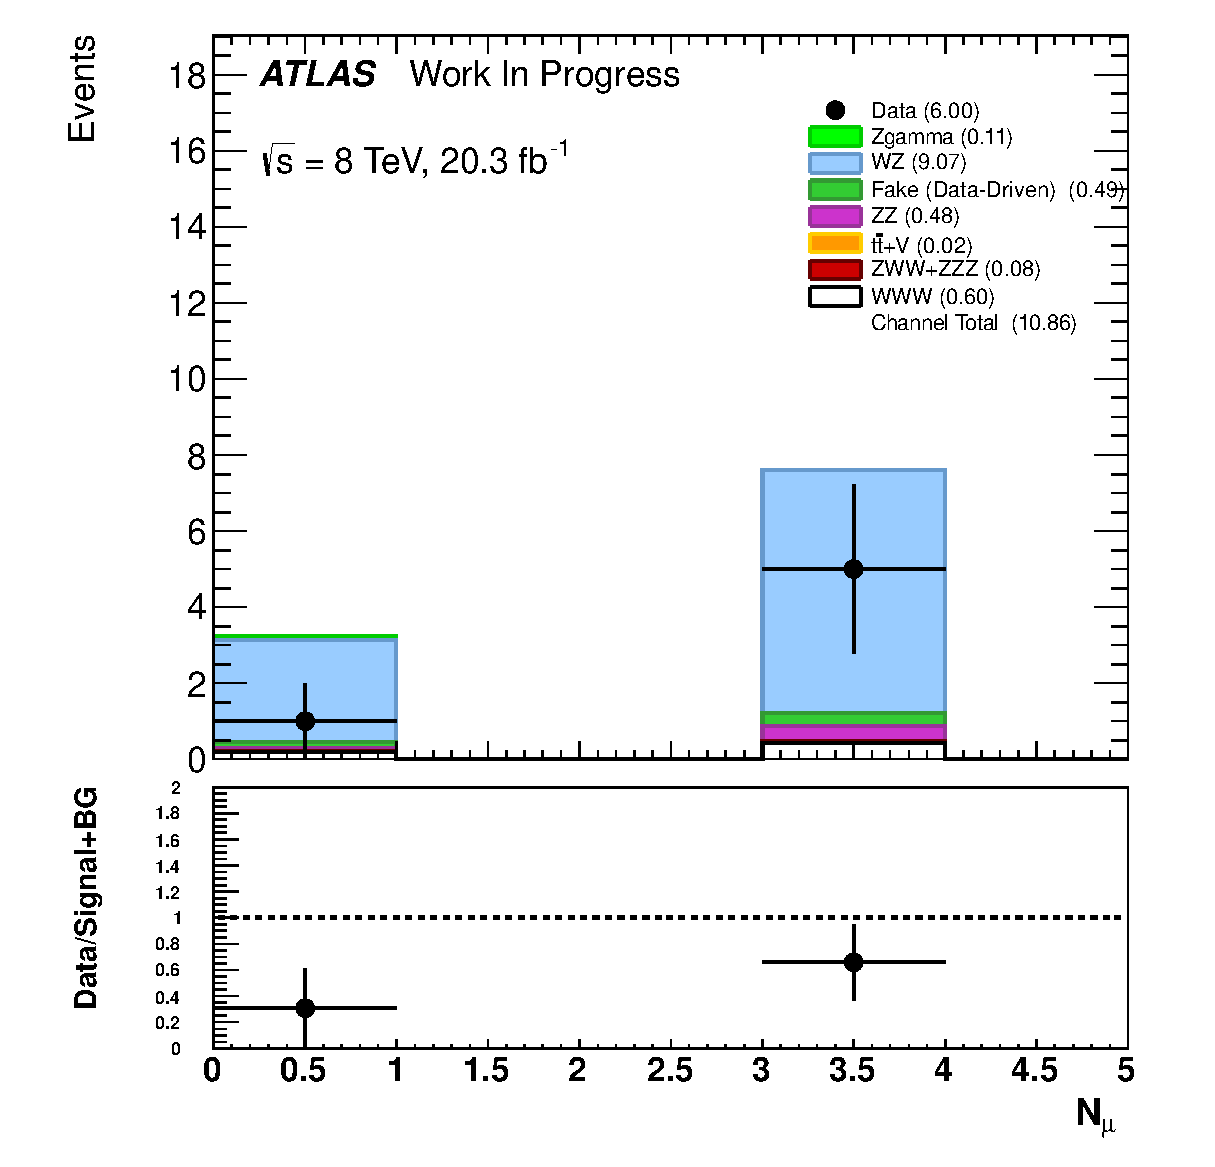
\includegraphics[width=0.3\columnwidth]{figures/appendix_signal_selection/PreselectionJune2_NoSTVF_2SFOS_ChargeAbs1_BVeto85_ZVeto20GeV_METGt55GeV_DeltaPhi2p5_NJetLt2_physics/weight_all/eps/NMuons_histratio.eps}
\caption{Distributions showing data compared to the signal plus background estimate in the 2 SFOS region at each stage 
of the selection before the cuts are applied to the given distribution. Plots should be read sequentially from left to right
and from top to bottom. 
Referring to Table~\ref{tab:cutflow_weighted_2sfos}, the top left
plot is shown before cut \#3 is applied, the top middle is before cut \#4, and
so on until the bottom right which is after all cuts are applied.}
\label{fig:2sfos}
\end{figure}

The 2 SFOS signal region has a similar background composition as
the 1 SFOS signal regions, since it is also dominated by 
the $WZ$ background.  As a result, the systematic uncertainties
on the signal and background are very similar to the 1 SFOS region.
However, 
as can be seen
in
\tab\ref{tab:cutflow_weighted_1sfos}
and 
\tab\ref{tab:cutflow_weighted_1sfos_bg},
the overall background prediction
is slightly smaller than the 1 SFOS signal region 
This is 
mainly because the tighter \MET~cut removes more of the $WZ$ background.
The signal and the 
fake background also contributes slightly less to the total
background but this is true
immediately after applying the SFOS requirement, and not
due to the \MET~cut.
The reason can be understood 
as described in \sec\ref{sec:signal_regions}:
there are twice many charge and flavor combinations to produce
1 SFOS pairs as there are 2 SFOS pairs.


From the cutflow tables we can also see that there is a defict in the data
compared to the prediction which appears after the \deltaphi~
selection. Looking at the distributions at each cut for 
the 2 SFOS region in \fig\ref{fig:2sfos},
one can clearly see the deficit occuring in the bin
furtherst to the right in the $|\deltaphi|$ distribution.
The deficit then propogates through uniformly in the 
\njet~and \nmu~distributions until the final estimate.
Note that the bin where the deficit occurs in the $|\deltaphi|$
distribution is also dominated by the $WZ$ background.
We have verified the modelling of the $WZ$ background
as a function of this quantity in control regions. 
Furthermore, the $|\deltaphi|$ distribution
shows good agreement in the 1 SFOS region at this stage
where it is also dominated by the $WZ$ background.
We have no reason to believe that the modelling of the $WZ$
background should be very different or should 
break down in the 2 SFOS region as compared to elsewhere.
Thus, the deficit is most likely a statistical fluctuation
and not due to a problem in the modelling of the 
background.
The Poisson probability of observing $\leq 6$ events
when 10.86 events are expected is 8.5\%.
Thus, even though this is the largest deviation observed in the signal
regions, it is still within 2 standard deviations (5\%).






\subsection{Correction Factors and Fiducial Cross-sections}
\label{sec:inputs}

The correction factor, $C_i$, is defined for each channel, $i$,
as the ratio of the number of expected signal events measured
at the reconstruction level, $N_i^{\textrm{Reco}}$, over the number
expected from truth information, $N_i^{\textrm{Truth}}$.
\begin{equation}
C_i = \frac{N_i^{\textrm{Reco}}}{N_i^{\textrm{Truth}}}
\end{equation}
$N_i^{\textrm{Reco}}$ 
is determined using the reconstruction
level selection described in \sec\ref{sec:signal_regions} and
listed in \tab\ref{tab:signal_selection};
$N_i^{\textrm{Truth}}$  is determined using the fiducial
selection described in \sec\ref{sec:fiducial} and 
listed in \tab\ref{tab:fiducial_selection}. The same generator, 
\vbfnlo, is used for both to remove any dependence on the 
cross-section or other generator specific effects.

The fiducial cross-sections are calculated also using the selection
from the \sec\ref{sec:signal_regions} after weighting
to the cross-section for the given sample. Recall also 
from \sec\ref{sec:signal} and \tab\ref{tab:signal_xsec}
that the fiducial cross-sections were generated using
both \madgraph~and \vbfnlo~and were shown to be in good agreement.
The fiducial cross-sections from \madgraph~are used in the final
estimates.

\begin{table}[ht!]
\centering
\begin{tabular}{|c||c|c|c|}
\hline
%& Channel & Signal Efficiency, $\varepsilon_i$  & Acceptance ($\times 10^{-4}$), $A_i$\\
 Channel & $C_i$   & Fiducial Cross-section [ab]\\
%&         & $\varepsilon_i$    &  $A_i$ \\
\hline\hline
0 SFOS &  $0.534 \pm .021$ & $123.6 \pm 4.7$\\
1 SFOS &  $0.500 \pm .018$ & $136.9 \pm 4.7$\\
2 SFOS &  $0.615 \pm .038$ & $48.8  \pm 2.9$ \\
\hline
\end{tabular}

\caption{Correction factors, $C_i$, and fiducial cross-sections derived
separately for each signal region. Correction factors are determined
using \vbfnlo~; fiducial cross-sections are determined
using \madgraph.}
\label{tab:inputs_3l}
\end{table}

The correction factors and fiducial cross-sections are 
summarized separately for each signal region in 
\tab\ref{tab:inputs_3l}.
Note that the sum of the fiducial cross-sections
in each signal region gives the combined fiducial cross-section
which was reported in \eqn\ref{eq:fiducial_theory} along with 
PDF and scale uncertainties.

